
To control the agreement of the Z+jets background prediction,
we compare the predictions of the relevant kinematic observables with the data.
We do this at the level of the $ZZ$ preselection cuts that were described in
Section \ref{sec:selection}. At this selection level we expect the Z+jets background
to be dominant.

Figure~\ref{fig:npv} shows the number of primary vertices in $ee$ and $\mu\mu$ final states 
after the $\ZZ$ preselections, comparing data to the simulation which was reweighted in the 
number of pile up events to match the values in data. This is a validation of the reweighting procedure. 
Figures~\ref{fig:zmass_zzpresel_mm}-\ref{fig:zmass_zzpresel_ee} show the dilepton mass distributions 
after applying all $\ZZ$ preselections except for the dilepton mass cuts, comparing data 
with simulation for the $\mu\mu$ amd $ee$ final states respectively in different jet 
bin final states. We observe in general a good agreement, except for a slight shift in the 
$\mu\mu$ final states. Figures~\ref{fig:zpt_zzpresel_mm} and~\ref{fig:zpt_zzpresel_ee} 
show the dilepton $p_T$ spectrum after the $\ZZ$ preselections for $\mu\mu$ and $ee$ final states. 
This provides an initial validation of the $\dyll$ background estimation. 

Table~\ref{tab:zzselection_all_4fb} shows the number of events observed in
data, comparing to the expected background contributions after the \zz\ preselections. 
The background estimation was discussed at Section~\ref{sec:backgrounds}. 
We validate the observables that are used in the higgs signal extraction at the 
$\ZZ$ preselection level. 
Figures~\ref{fig:met_zzpresel_mm}-\ref{fig:dphijetmet_zzpresel_ee} show 
the data to simulation comparions of the $\met$, $M_T$ and $\Delta\phi(jet,met)$ distributions. 
Good agreement between data and simulation is observed. 

%%%%%%%%%%%%%%%%%%
\begin{table}[!ht]
\begin{center}
\begin{tabular}{c|c|c|c}
\hline
WW/Top       & 137.63 $\pm$ 8.73 & 111.28 $\pm$ 7.06 & 248.91 $\pm$ 11.23 \\       
\zz\         & 62.18 $\pm$ 0.29  & 41.81 $\pm$ 0.23  & 103.99 $\pm$ 0.37 \\       
$gg\to ZZ$   & 5.59 $\pm$ 0.03   & 3.75 $\pm$ 0.02   & 9.33 $\pm$ 0.03 \\        
$\WZ$        & 53.84 $\pm$ 0.48  & 36.91 $\pm$ 0.39  & 90.75 $\pm$ 0.62 \\ 
Zjets        & 1008.05 $\pm$ 20.81   & 695.71 $\pm$ 13.79    & 1703.76 $\pm$ 24.97 \\ 
\hline
Total Background    & 1267.29 $\pm$ 22.57   & 889.45 $\pm$ 15.50    & 2156.74 $\pm$ 27.39 \\
\hline
DATA         & 1246   & 963  & 2209  \\ \hline
\end{tabular}
\caption{Expected number of signal and background events corresponding to an 
integrated luminosity of \intlumi after applying the \zz\ preselection requirements. 
Only statistical uncertaities are reported. The $\Wjets$ background is neglible thus omitted in the table.
%The background predictions do not have the data-to-simulation scale factors applied. 
}
\label{tab:zzselection_all_4fb}
\end{center}
\end{table}
%%%%%%%%%%%%%%%%%%

%%%%%%%%
\begin{figure}[!hbtp]
\begin{center}
\subfigure[Inclusive]{\label{subfig:npv_mm}
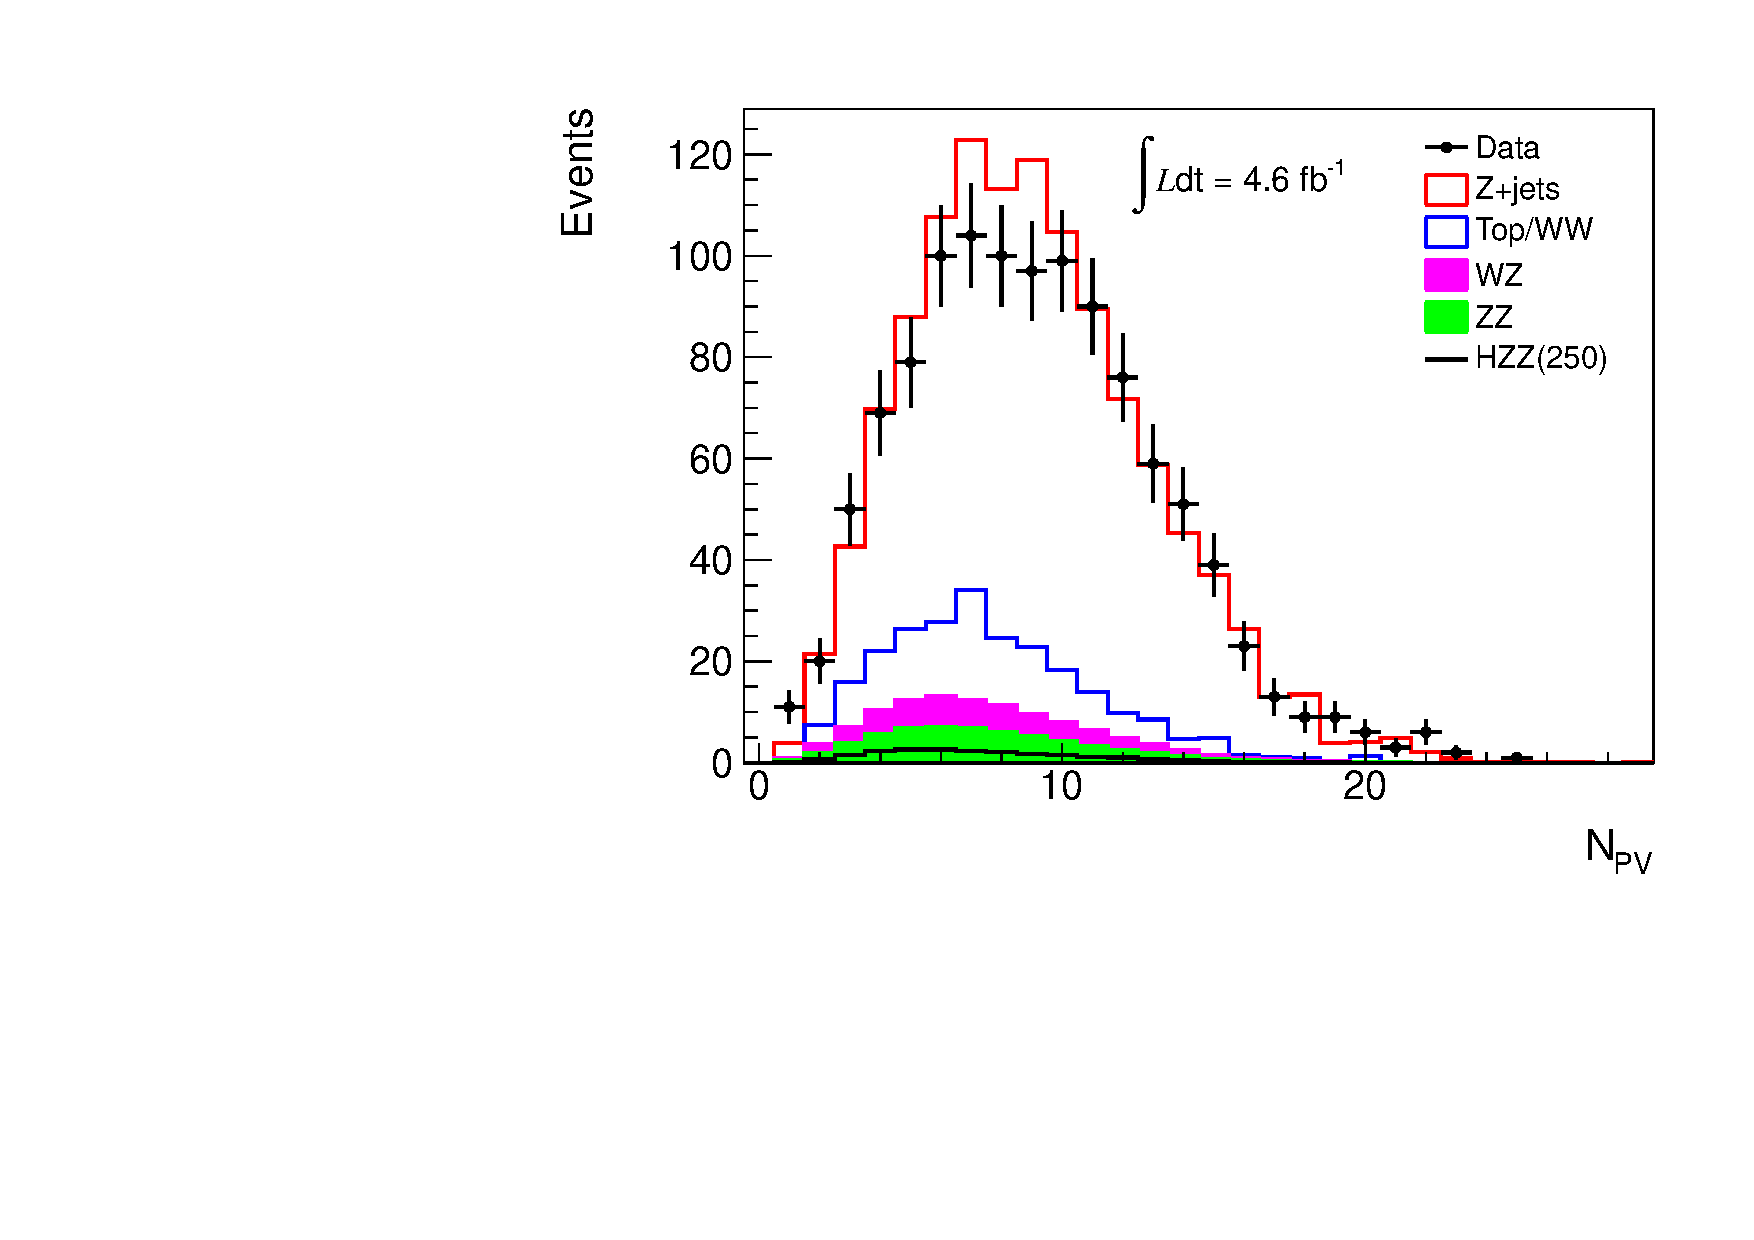
\includegraphics[width=.4\textwidth]{figures/presel_mH250_mm_npv.pdf}}
\subfigure[1-Jet]{\label{subfig:npv_ee}
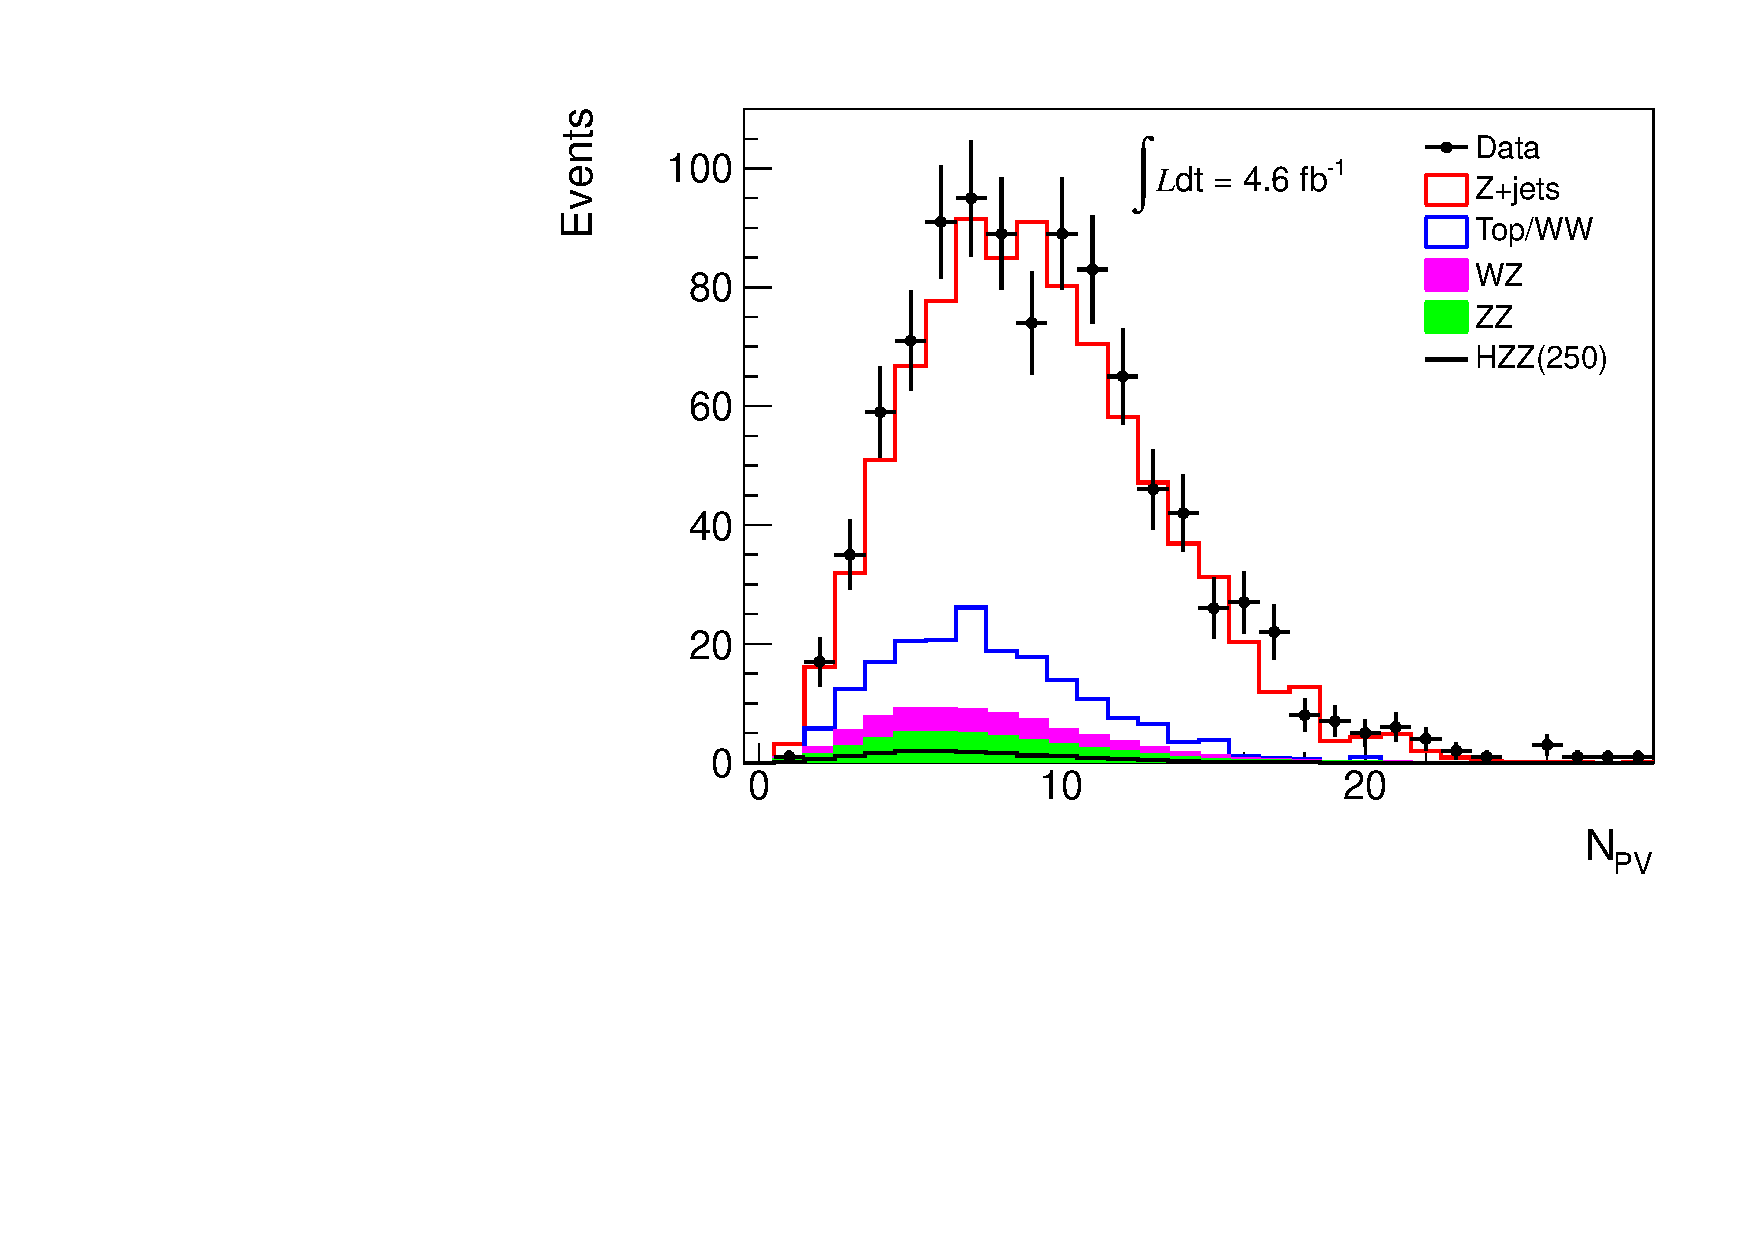
\includegraphics[width=.4\textwidth]{figures/presel_mH250_ee_npv.pdf}}
\caption{Distribution for the number of reconstructed primary vertices after the $\ZZ$ preselection observed in data corresponding 
to $4.6$~\ifb data in the muon~\subref{subfig:npv_mm} and electron~\subref{subfig:npv_ee} channels, compared to the expected from simulation for signal 
and background. The MC backgrounds are scaled as appropriate and the photon+jets estimate of the Z+jets background is added to the stack.}
\label{fig:npv}
\end{center}
\end{figure}
%%%%%%%%

%%%%%%%%
\begin{figure}[!hbtp]
\begin{center}
\subfigure[Inclusive]{\label{subfig:zmass_mm_incl}
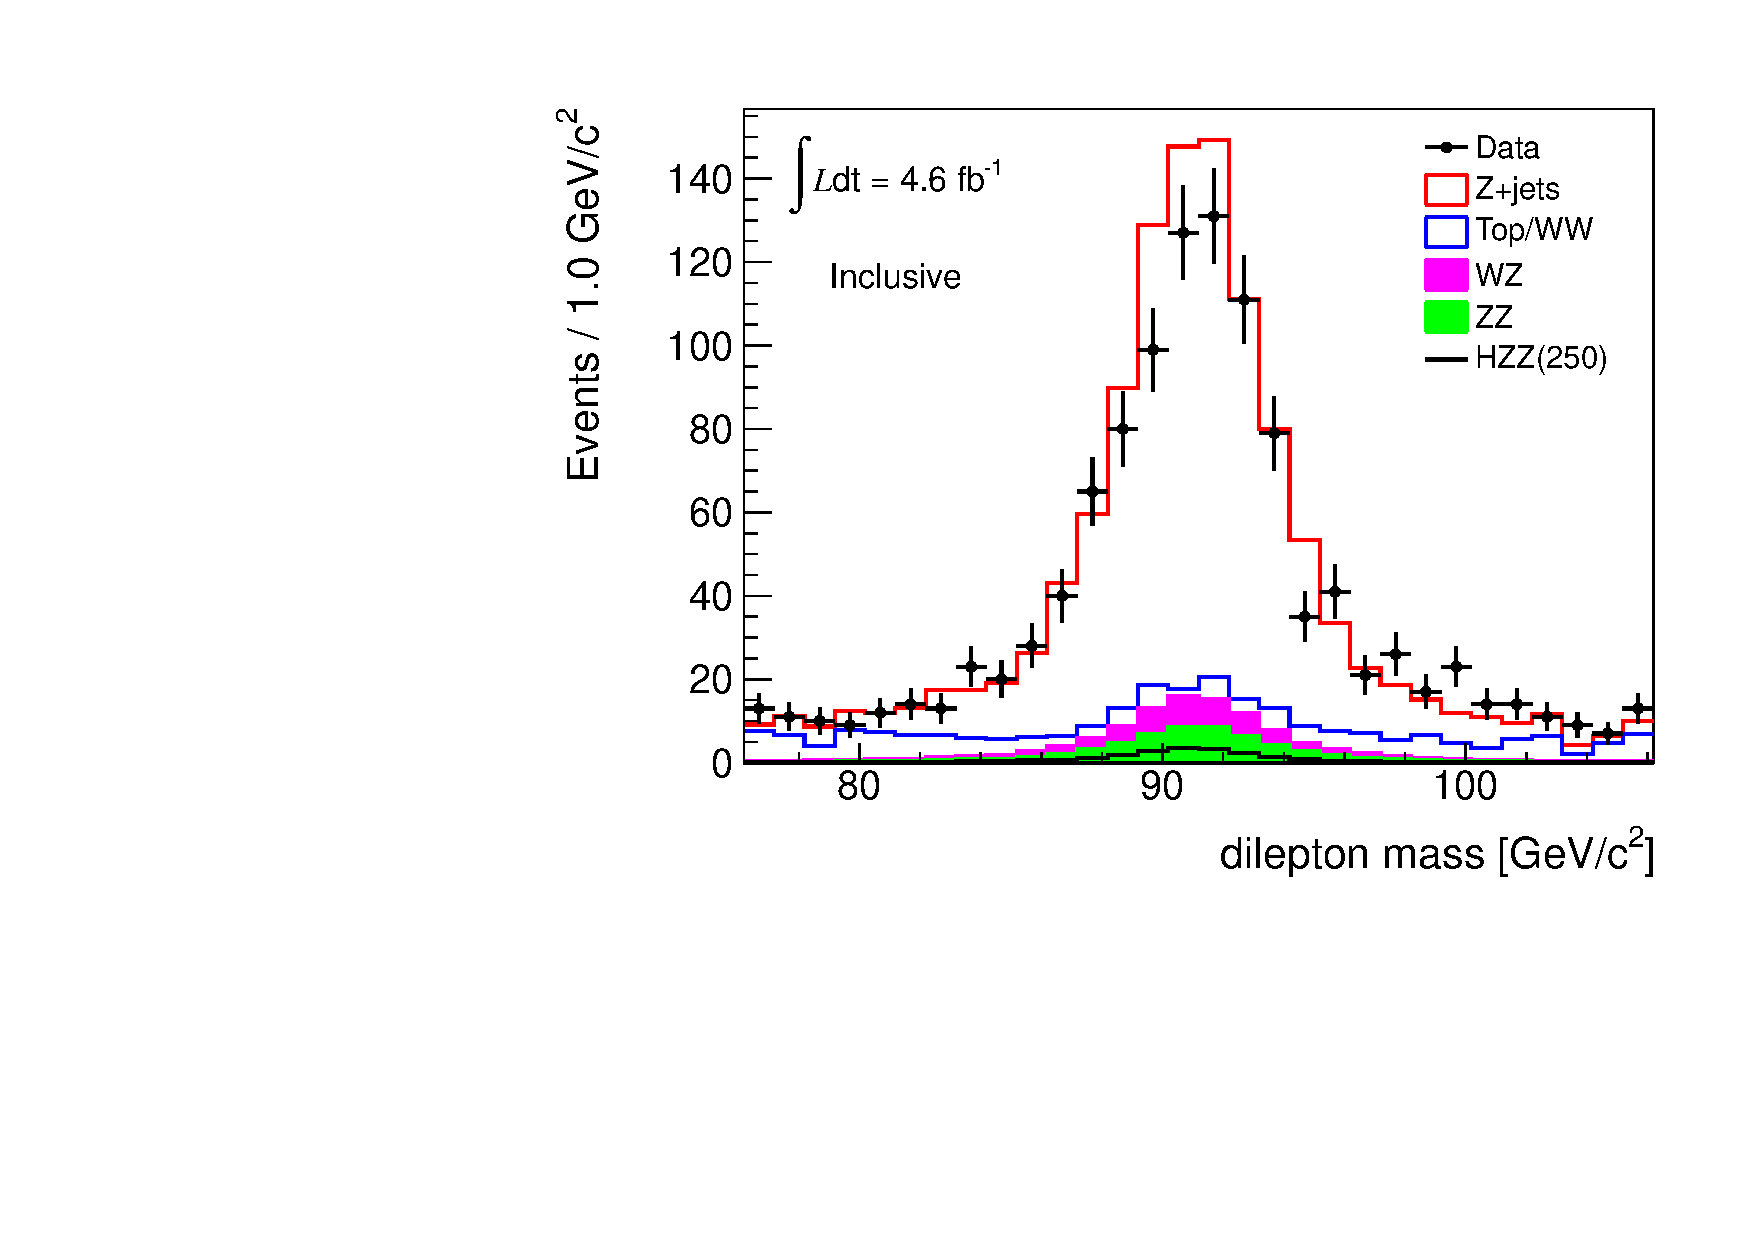
\includegraphics[width=.4\textwidth]{figures/presel_mH250_mm_mass_incl.pdf}}
\subfigure[0-Jet]{\label{subfig:zmass_mm_0j}
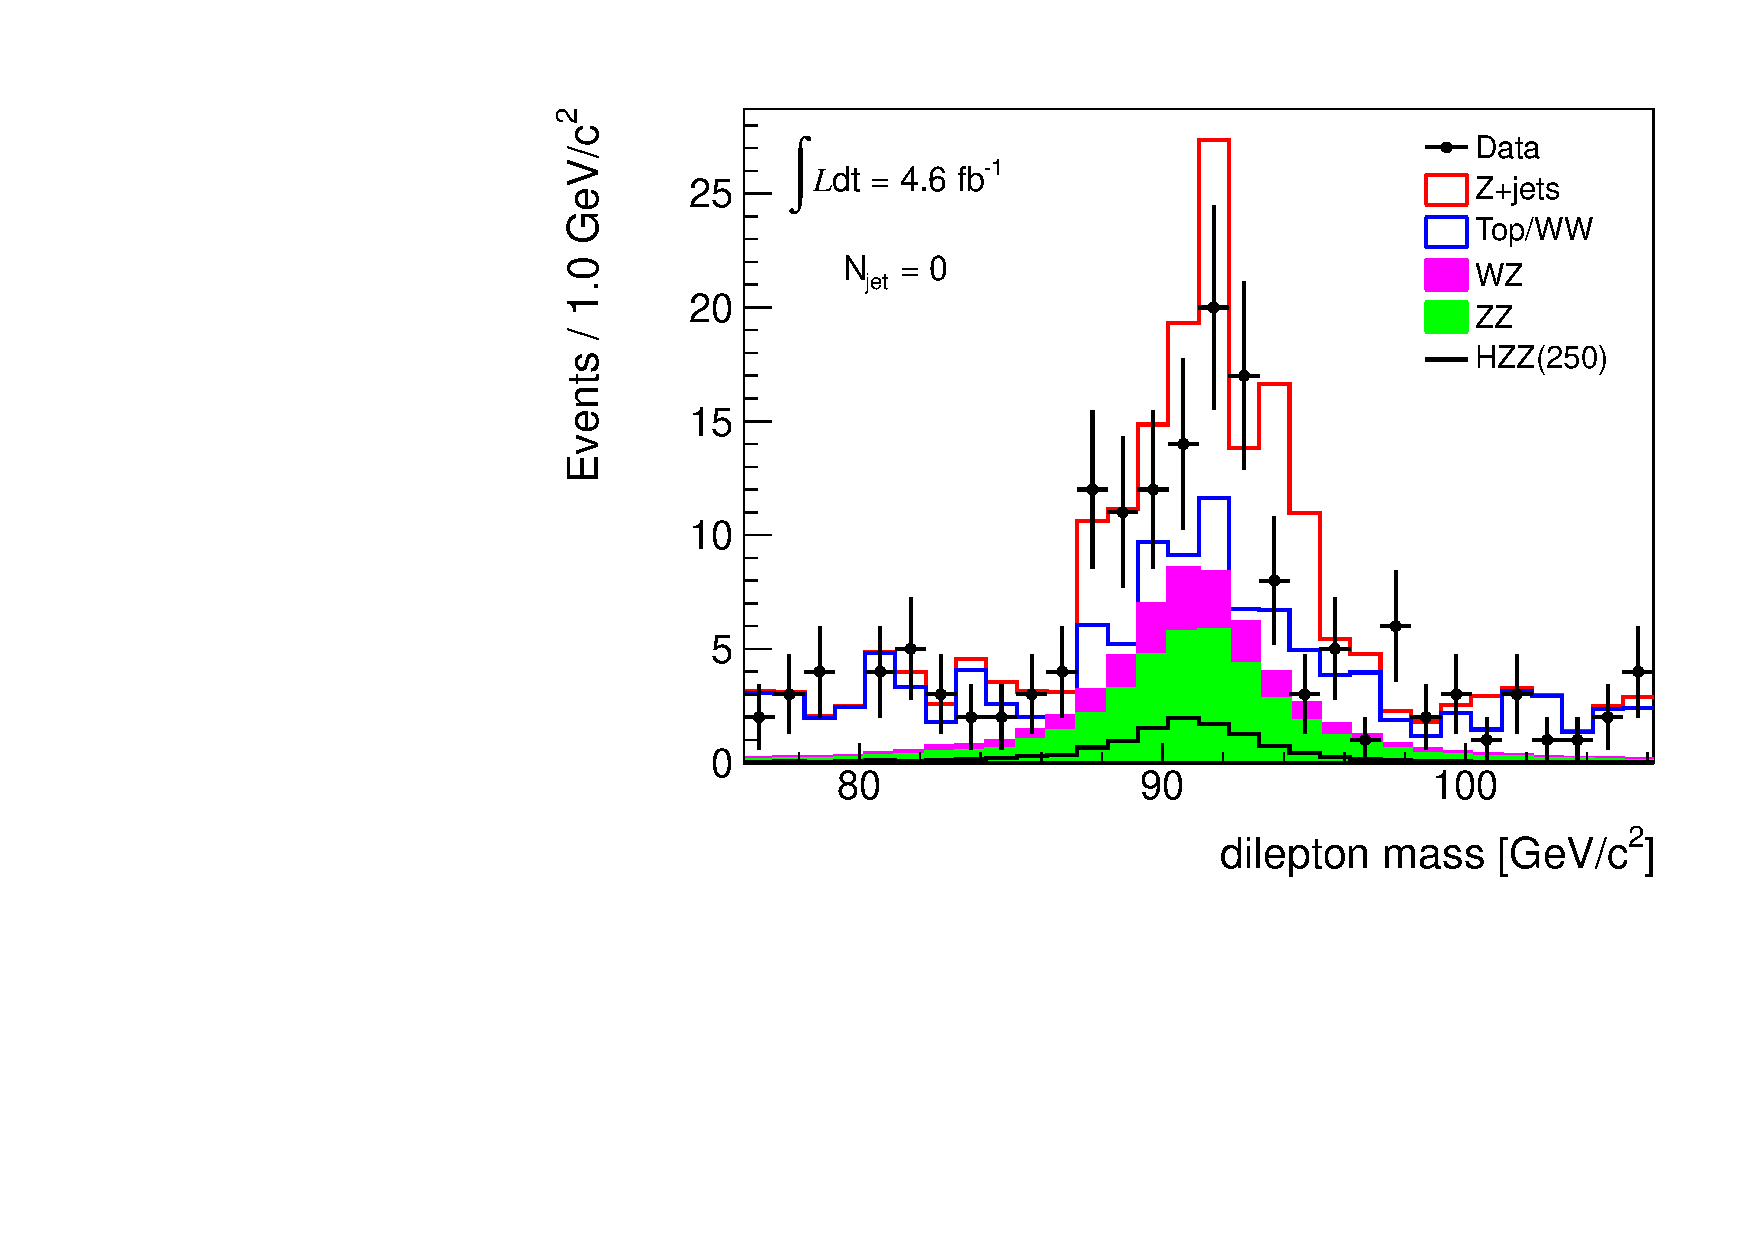
\includegraphics[width=.4\textwidth]{figures/presel_mH250_mm_mass_0j.pdf}} \\
\subfigure[1-Jet]{\label{subfig:zmass_mm_1j}
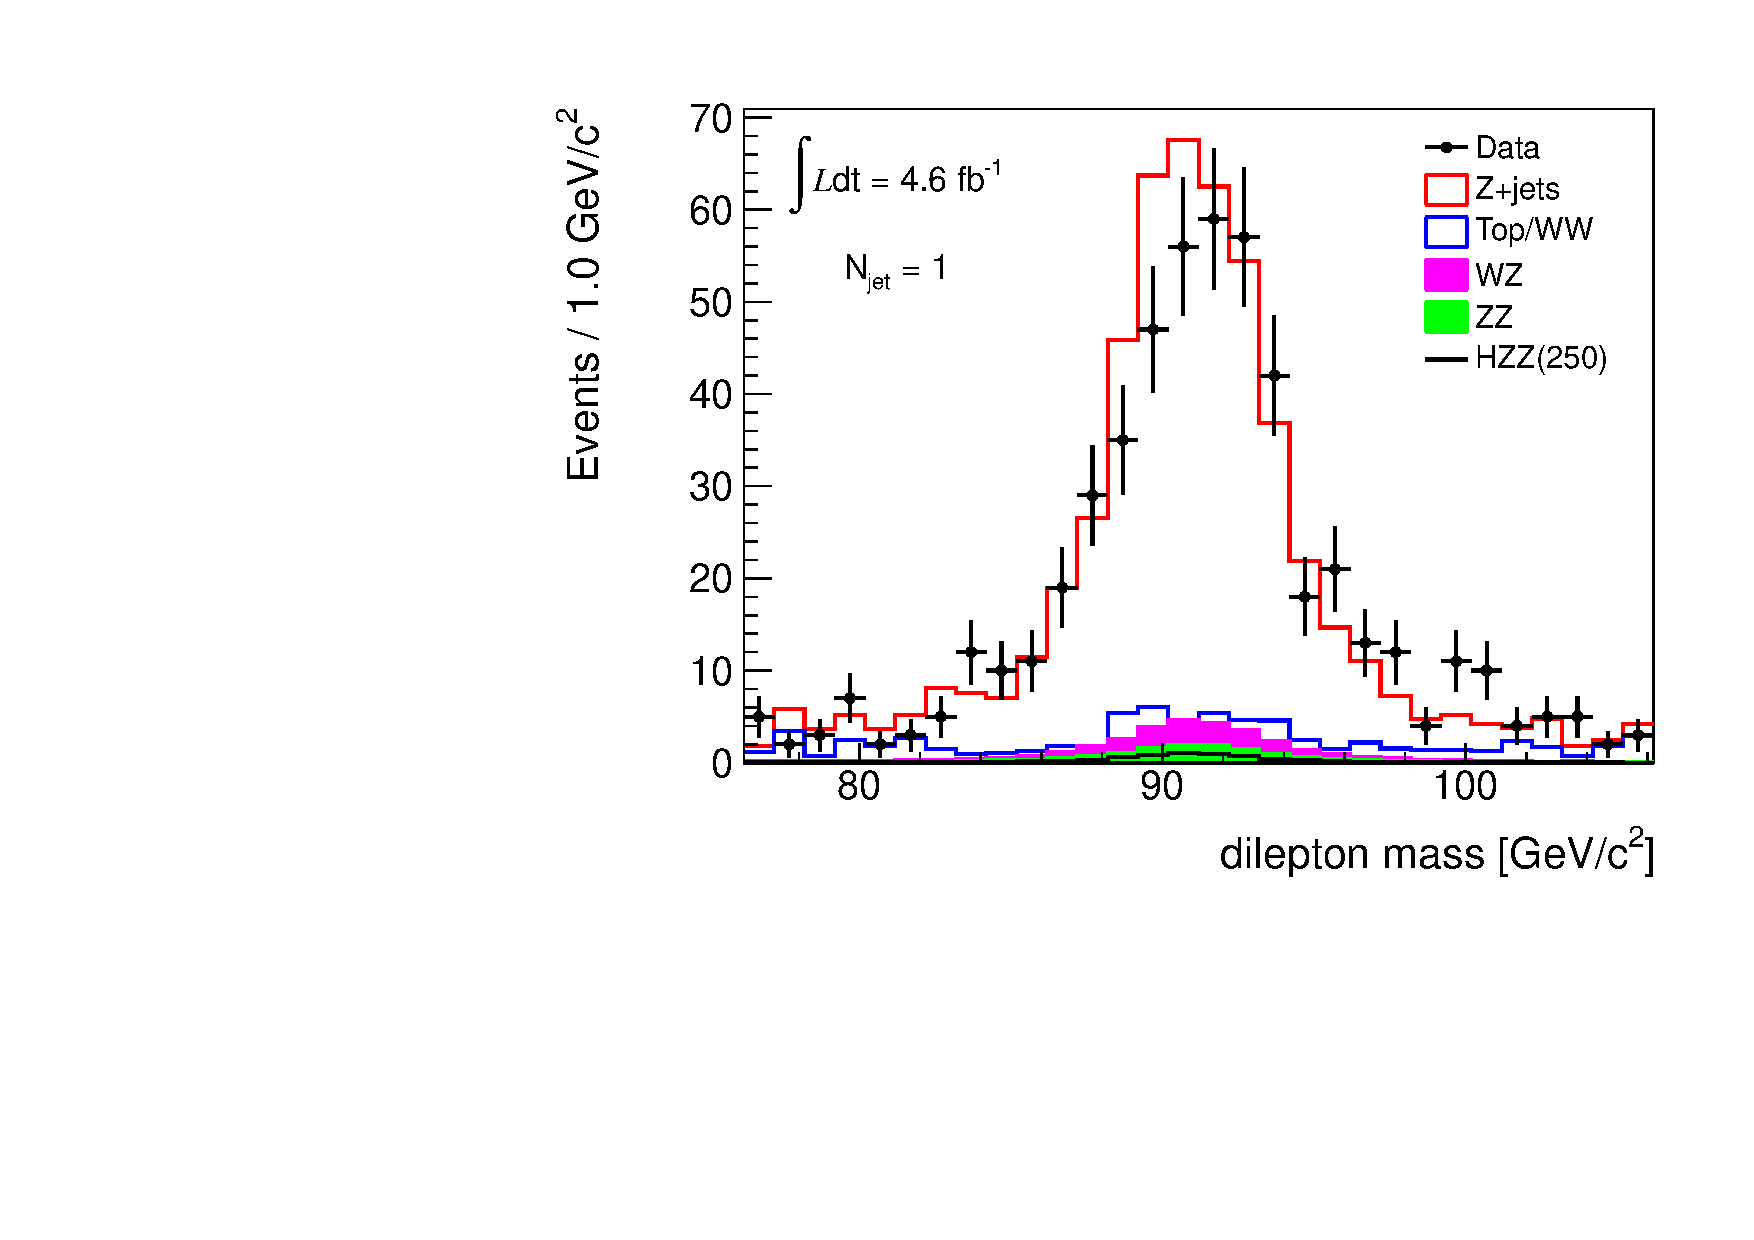
\includegraphics[width=.4\textwidth]{figures/presel_mH250_mm_mass_1j.pdf}}
\subfigure[$\geq$2 Jets]{\label{subfig:zmass_mm_2j}
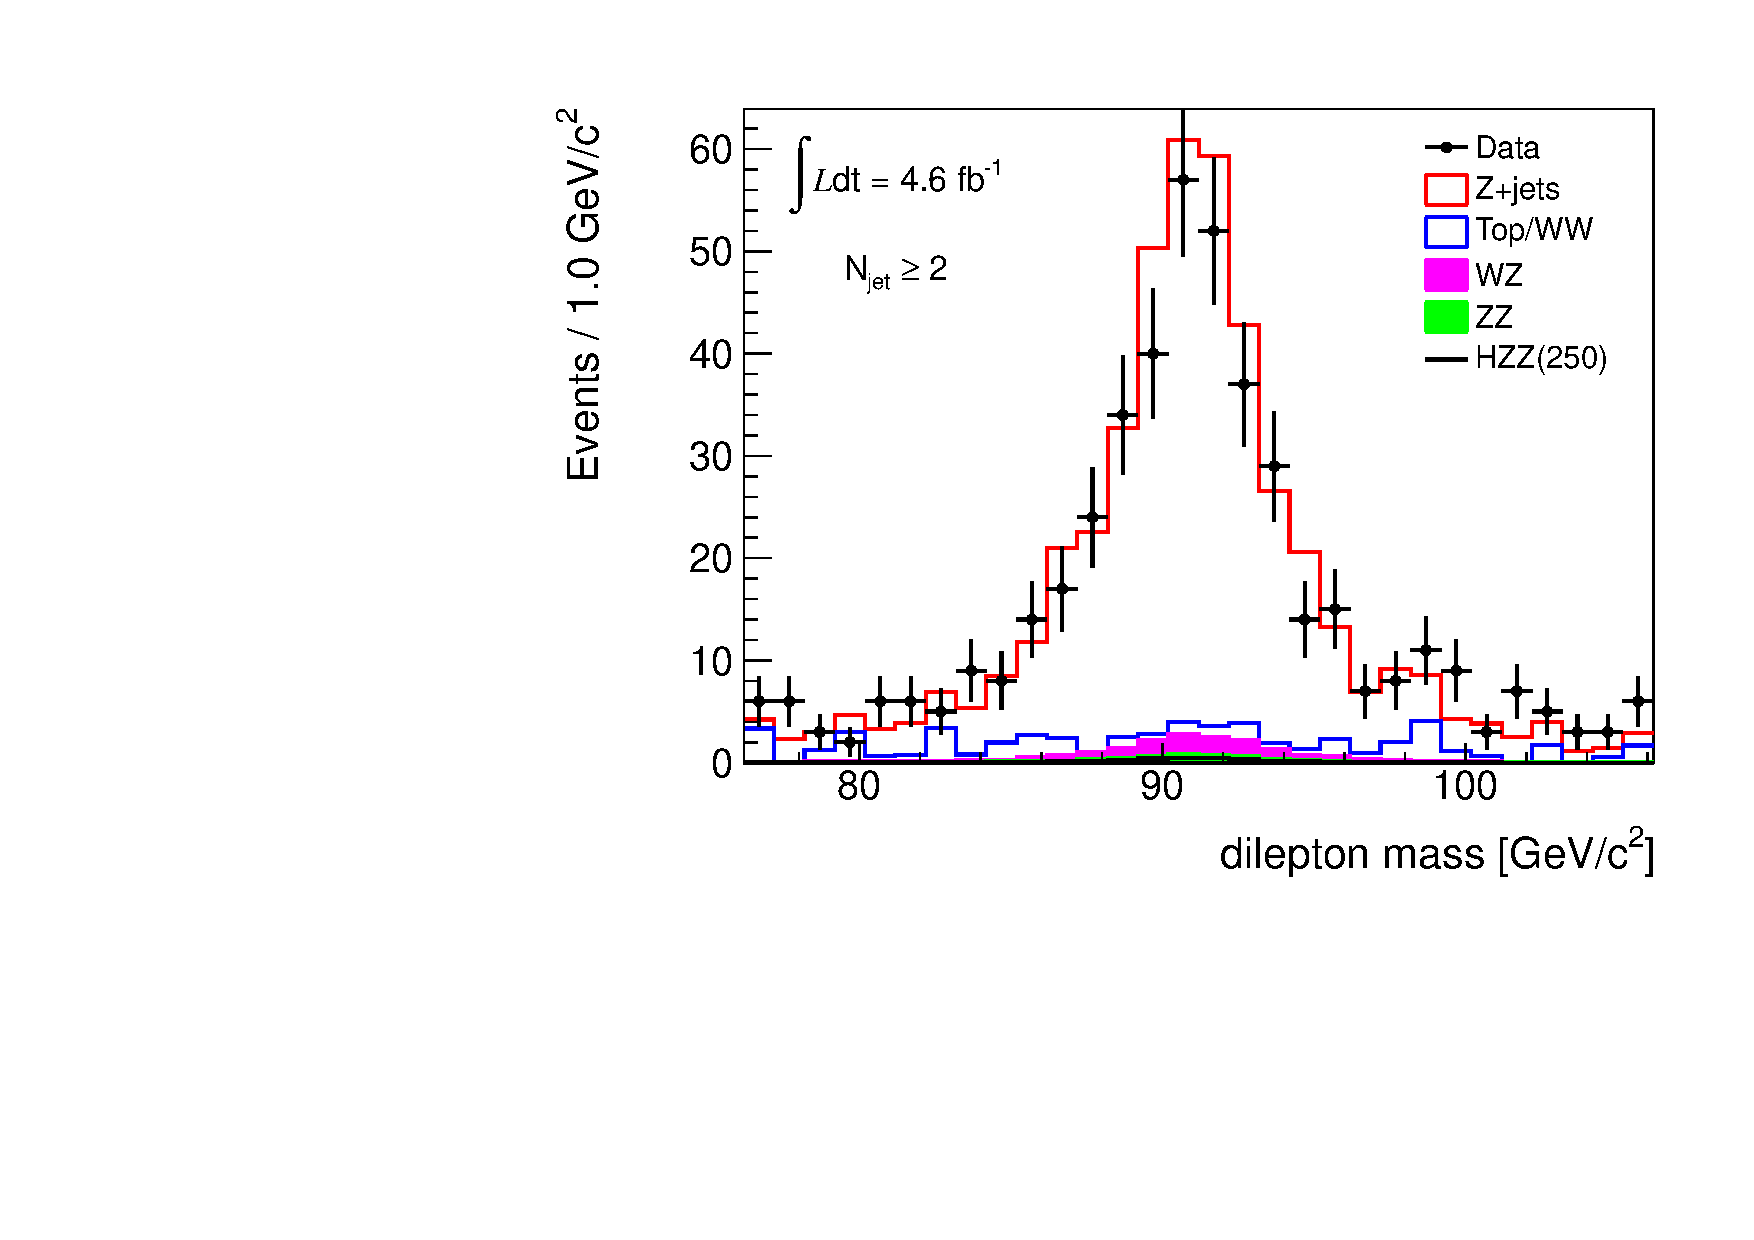
\includegraphics[width=.4\textwidth]{figures/presel_mH250_mm_mass_2j.pdf}}
\caption{Dilepton mass distribution in the muon channel after the $\ZZ$ preselection observed in data corresponding to $4.6$~\ifb data in 
the Inclusive~\subref{subfig:zmass_mm_incl}, 0-Jet~\subref{subfig:zmass_mm_0j}, 1-Jet~\subref{subfig:zmass_mm_1j} and $\geq$2-Jets~\subref{subfig:zmass_mm_2j} bins, 
compared to the expected from simulation for signal and background. The MC backgrounds are scaled as appropriate and the photon+jets estimate of the 
Z+jets background is added to the stack.}
\label{fig:zmass_zzpresel_mm}
\end{center}
\end{figure}
%%%%%%%%

%%%%%%%%
\begin{figure}[!hbtp]
\begin{center}
\subfigure[Inclusive]{\label{subfig:zmass_ee_incl}
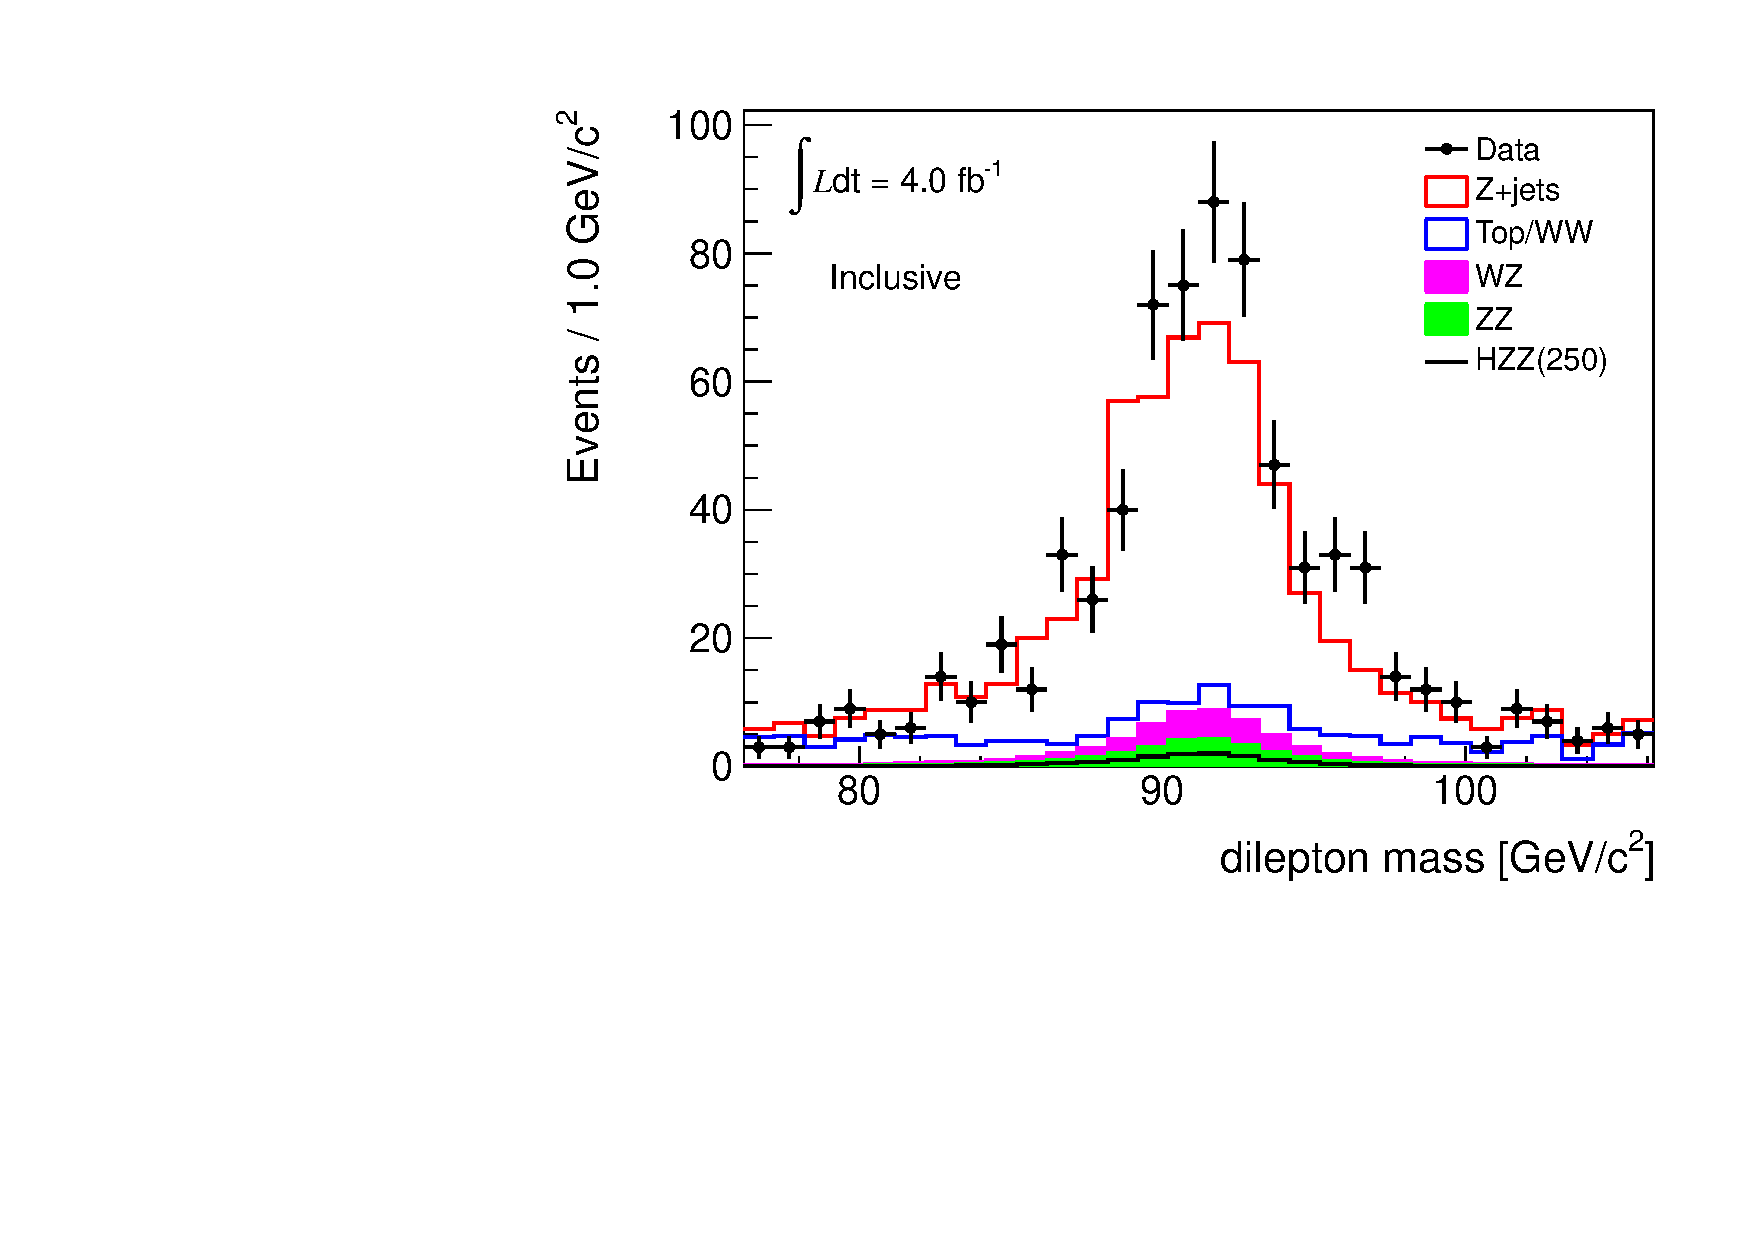
\includegraphics[width=.4\textwidth]{figures/presel_mH250_ee_mass_incl.pdf}}
\subfigure[0-Jet]{\label{subfig:zmass_ee_0j}
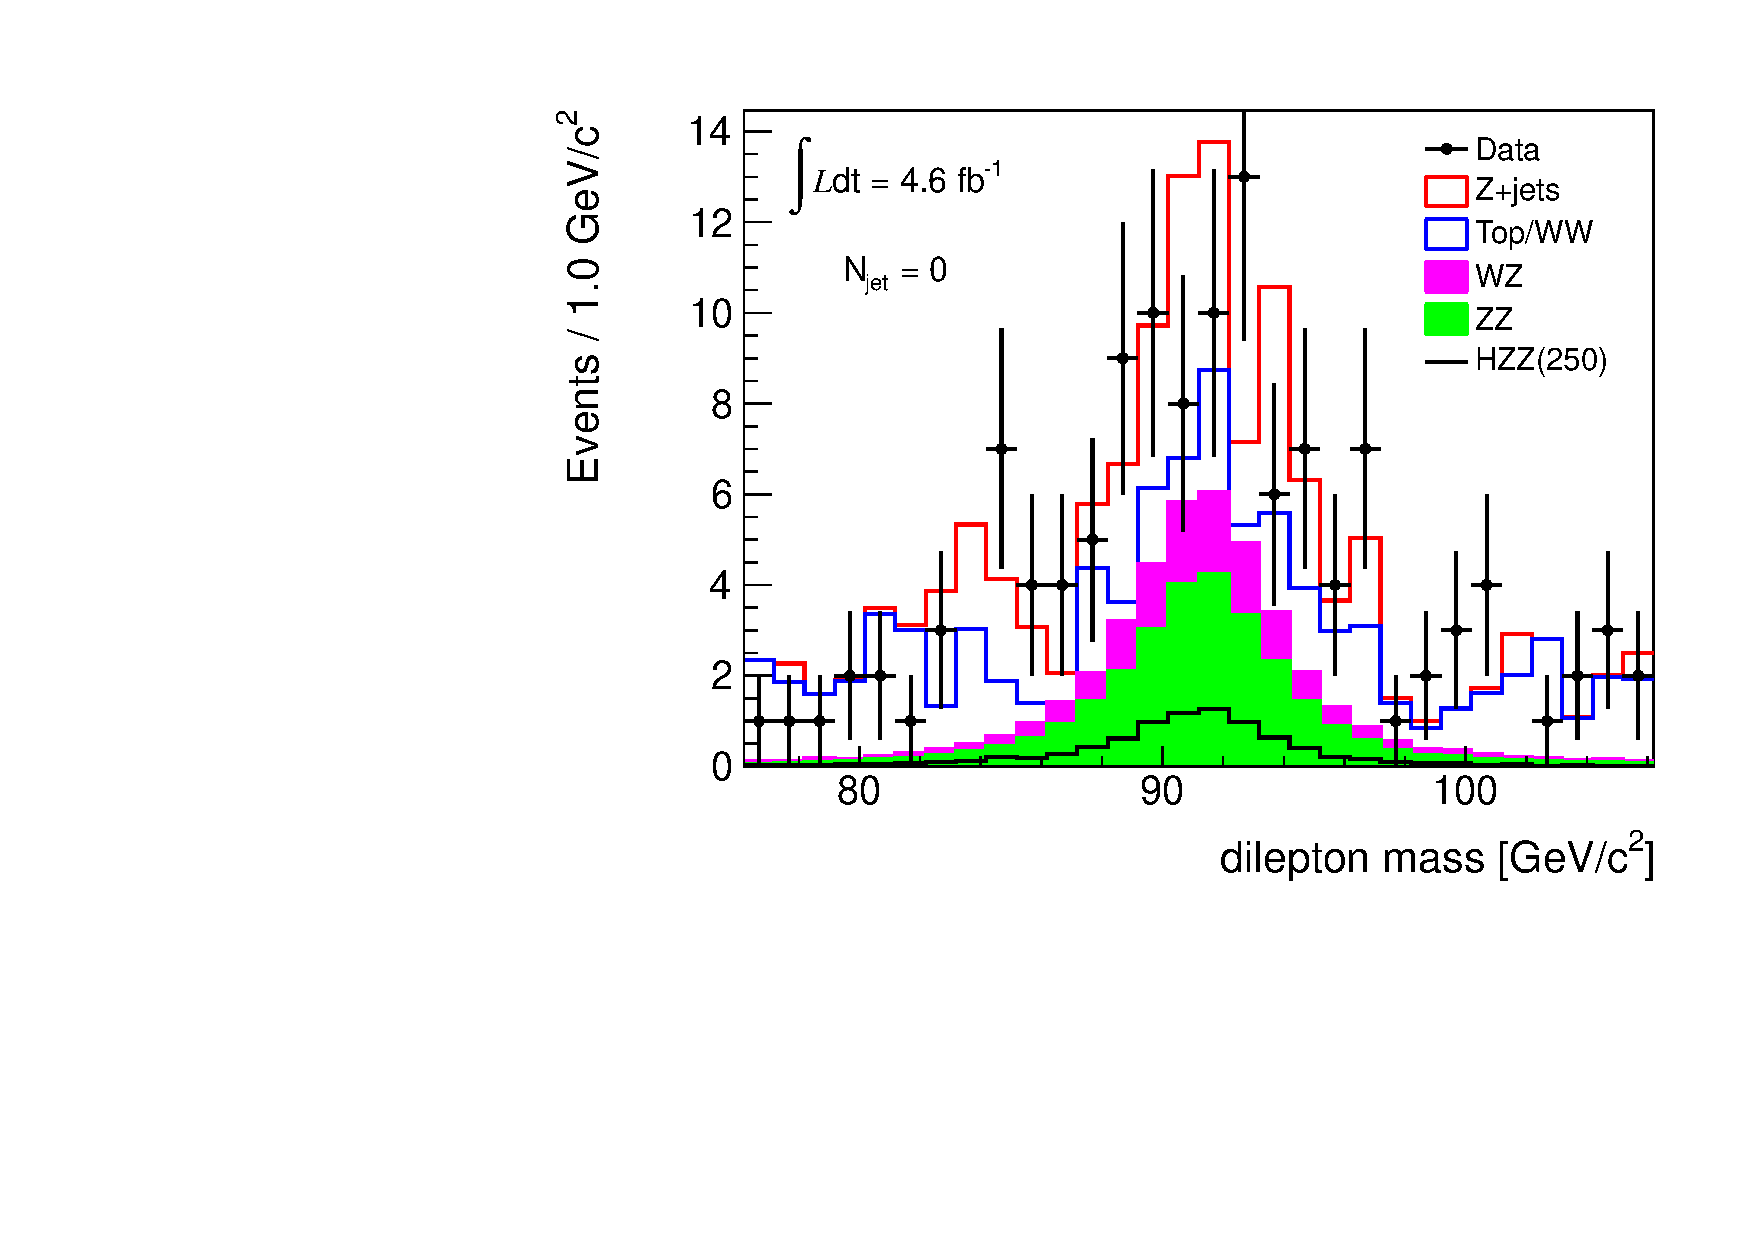
\includegraphics[width=.4\textwidth]{figures/presel_mH250_ee_mass_0j.pdf}} \\
\subfigure[1-Jet]{\label{subfig:zmass_ee_1j}
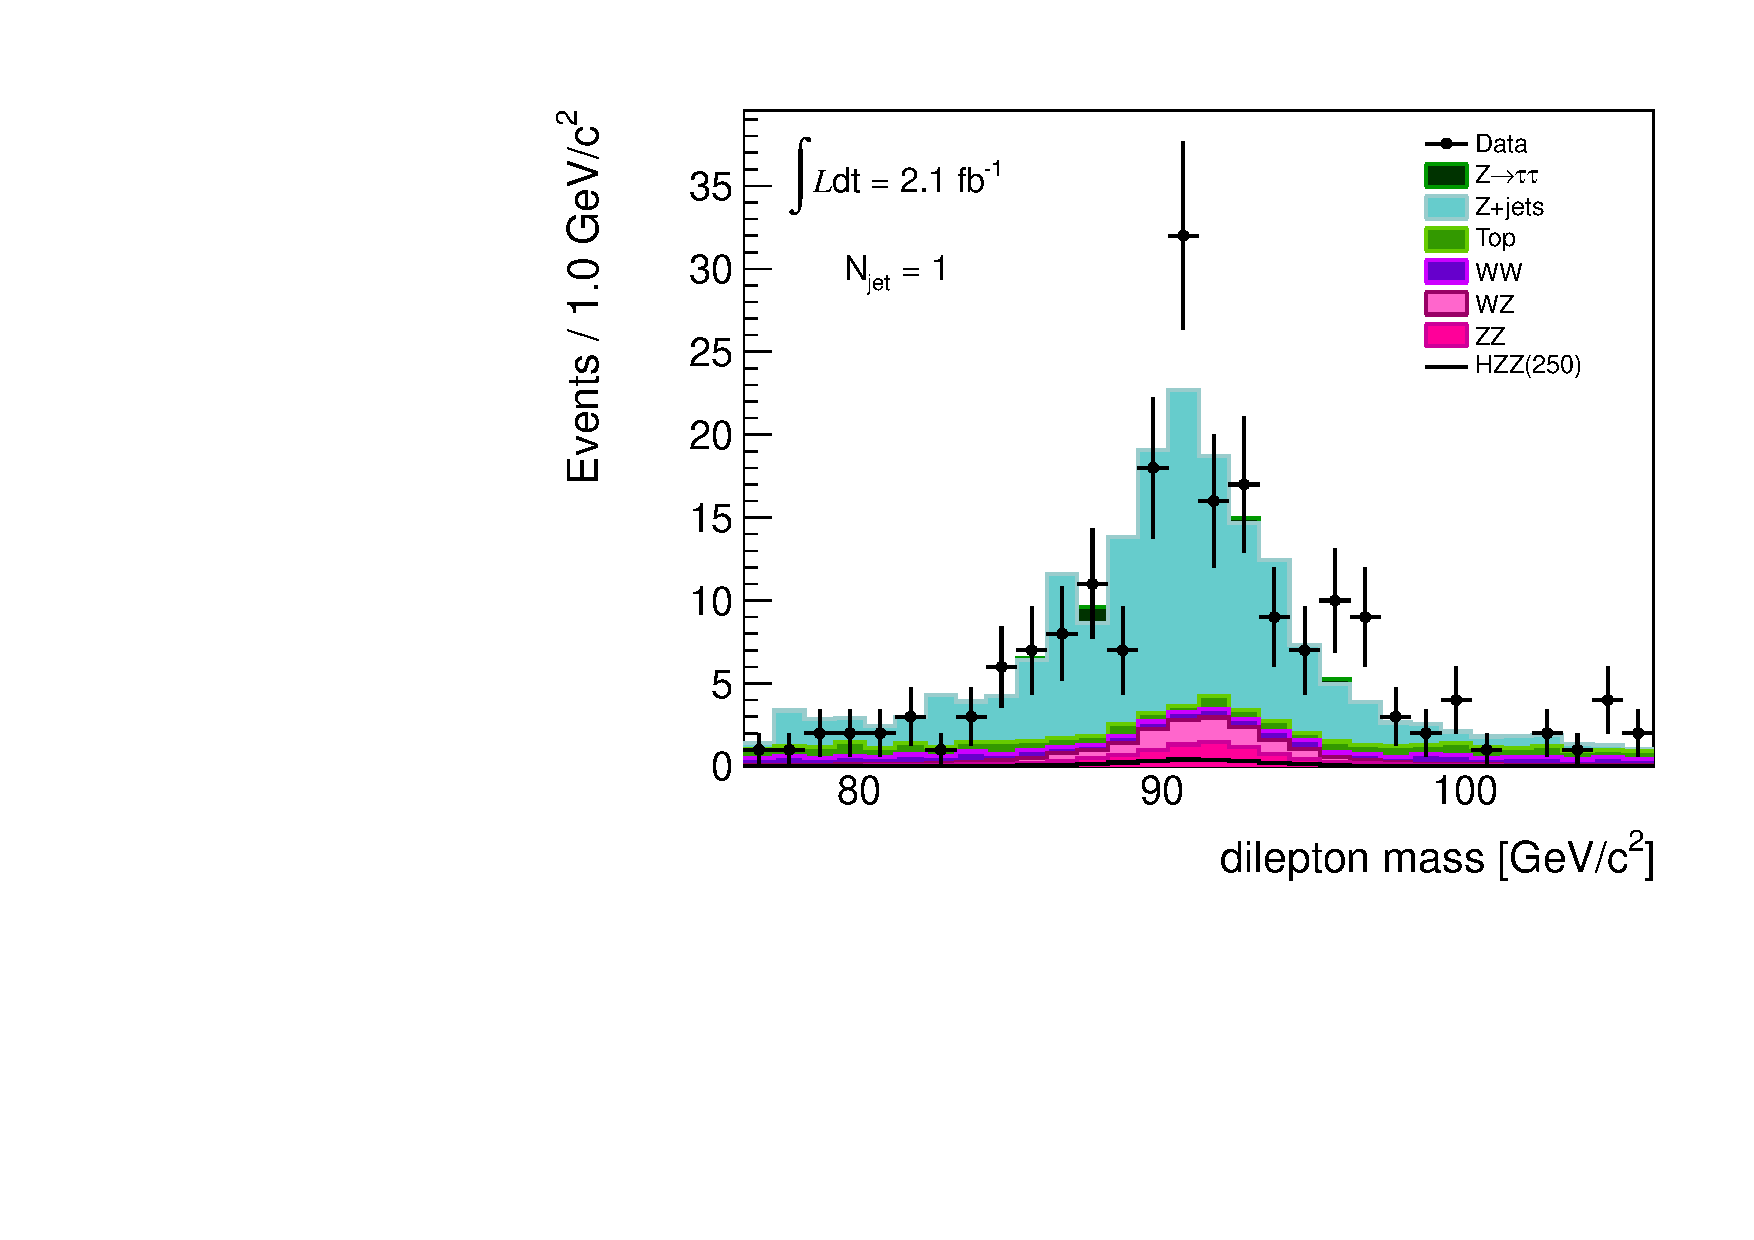
\includegraphics[width=.4\textwidth]{figures/presel_mH250_ee_mass_1j.pdf}}
\subfigure[$\geq$2 Jets]{\label{subfig:zmass_ee_2j}
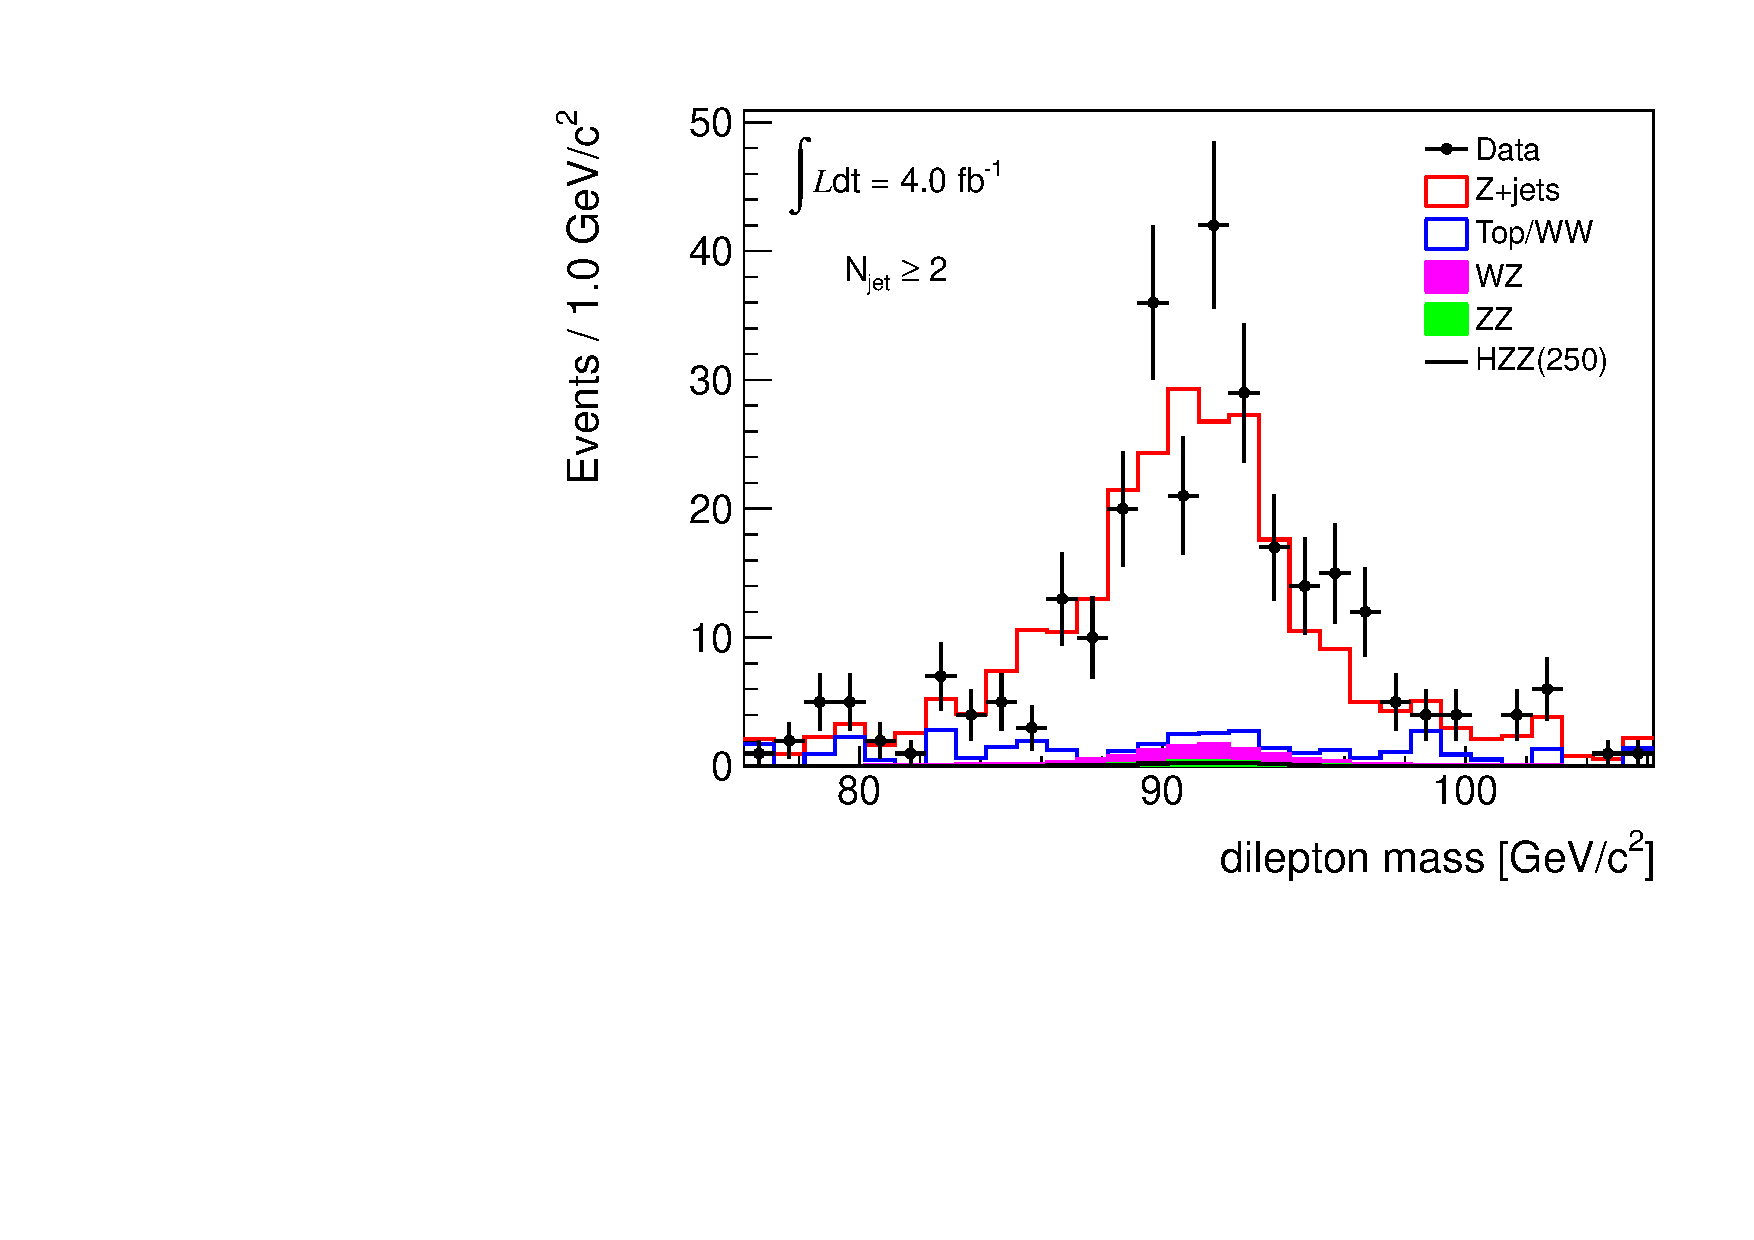
\includegraphics[width=.4\textwidth]{figures/presel_mH250_ee_mass_2j.pdf}}
\caption{Dilepton mass distribution in the electron channel after the $\ZZ$ preselection observed in data corresponding to $4.6$~\ifb data in 
the Inclusive~\subref{subfig:zmass_ee_incl}, 0-Jet~\subref{subfig:zmass_ee_0j}, 1-Jet~\subref{subfig:zmass_ee_1j} and $\geq$2-Jets~\subref{subfig:zmass_ee_2j} bins, 
compared to the expected from simulation for signal and background. The MC backgrounds are scaled as appropriate and the photon+jets estimate of the 
Z+jets background is added to the stack.}
\label{fig:zmass_zzpresel_ee}
\end{center}
\end{figure}
%%%%%%%%

%%%%%%%%
\begin{figure}[!hbtp]
\begin{center}
\subfigure[Inclusive]{\label{subfig:zpt_mm_incl}
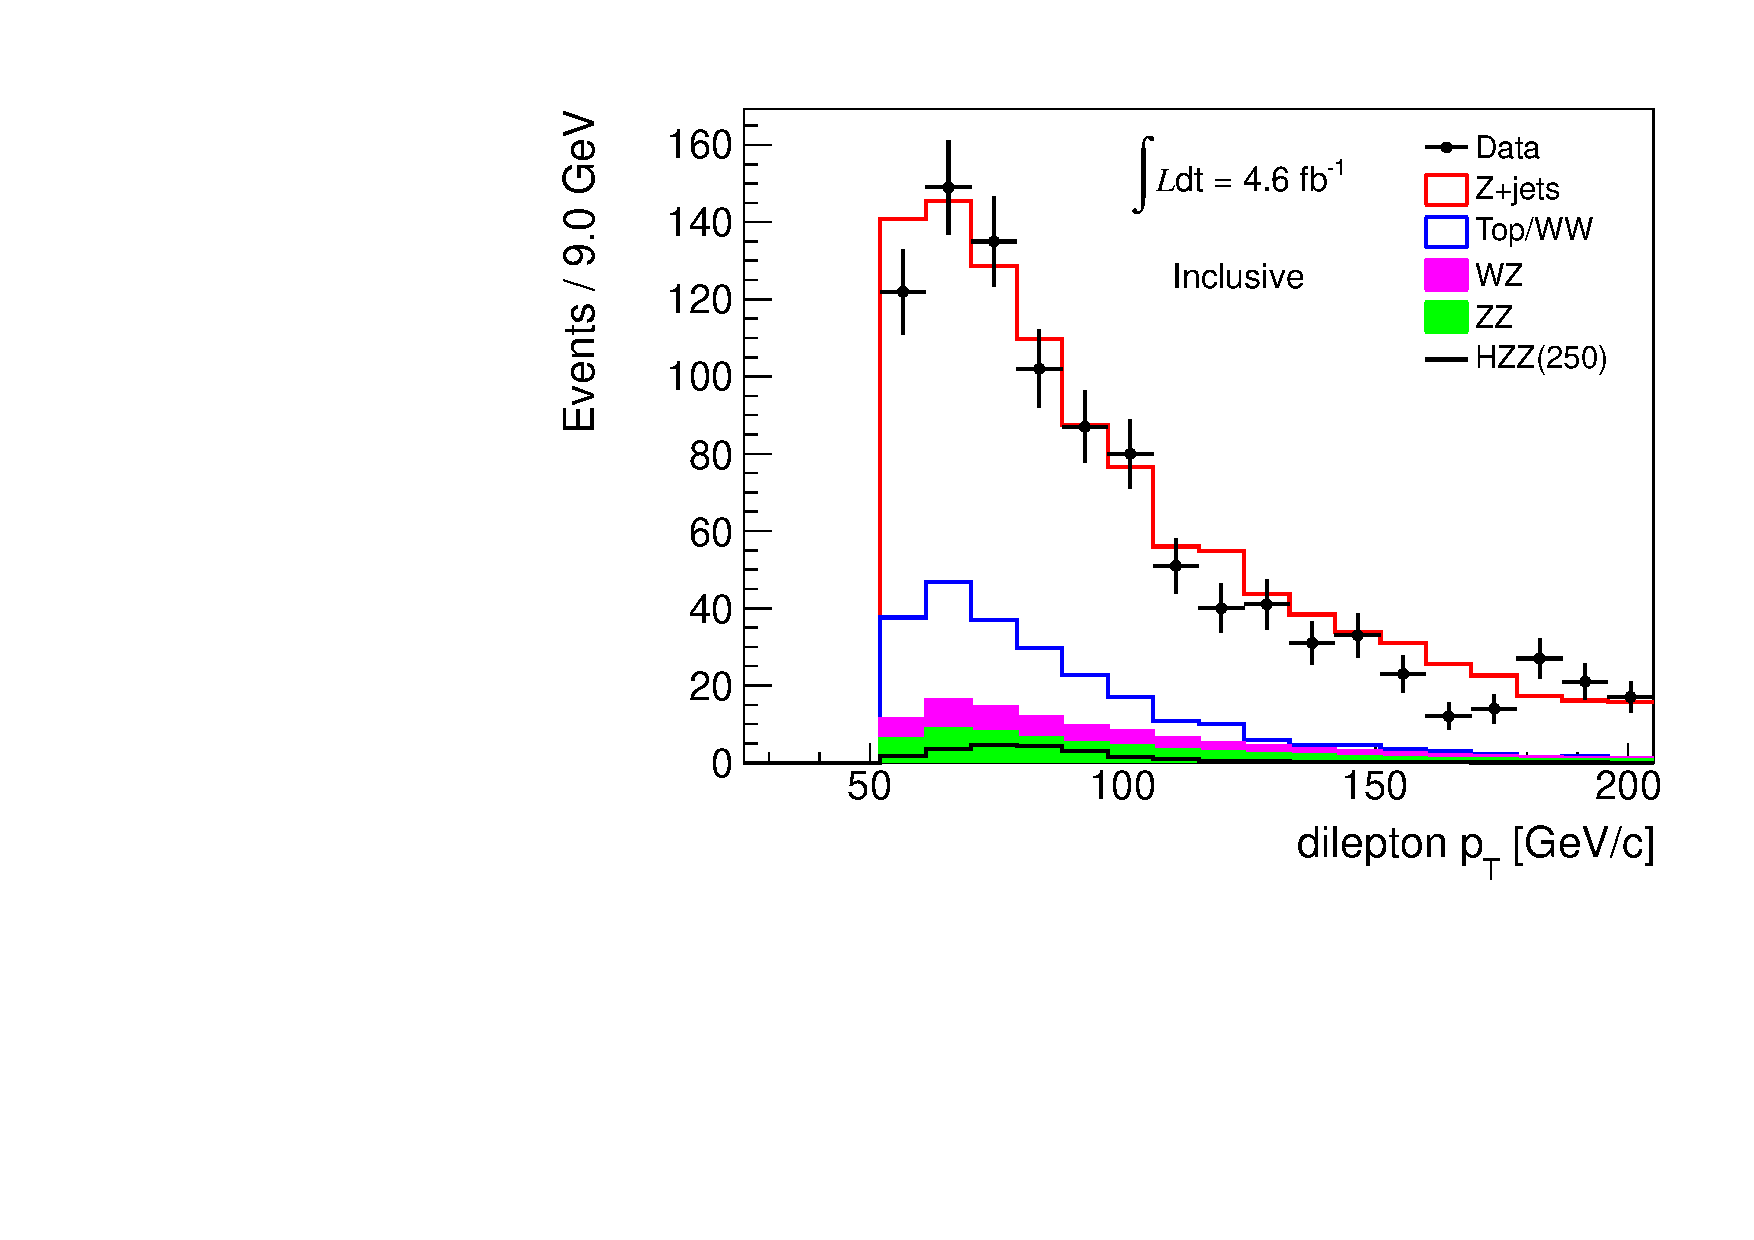
\includegraphics[width=.4\textwidth]{figures/presel_mH250_mm_dileppt_incl.pdf}}
\subfigure[0-Jet]{\label{subfig:zpt_mm_0j}
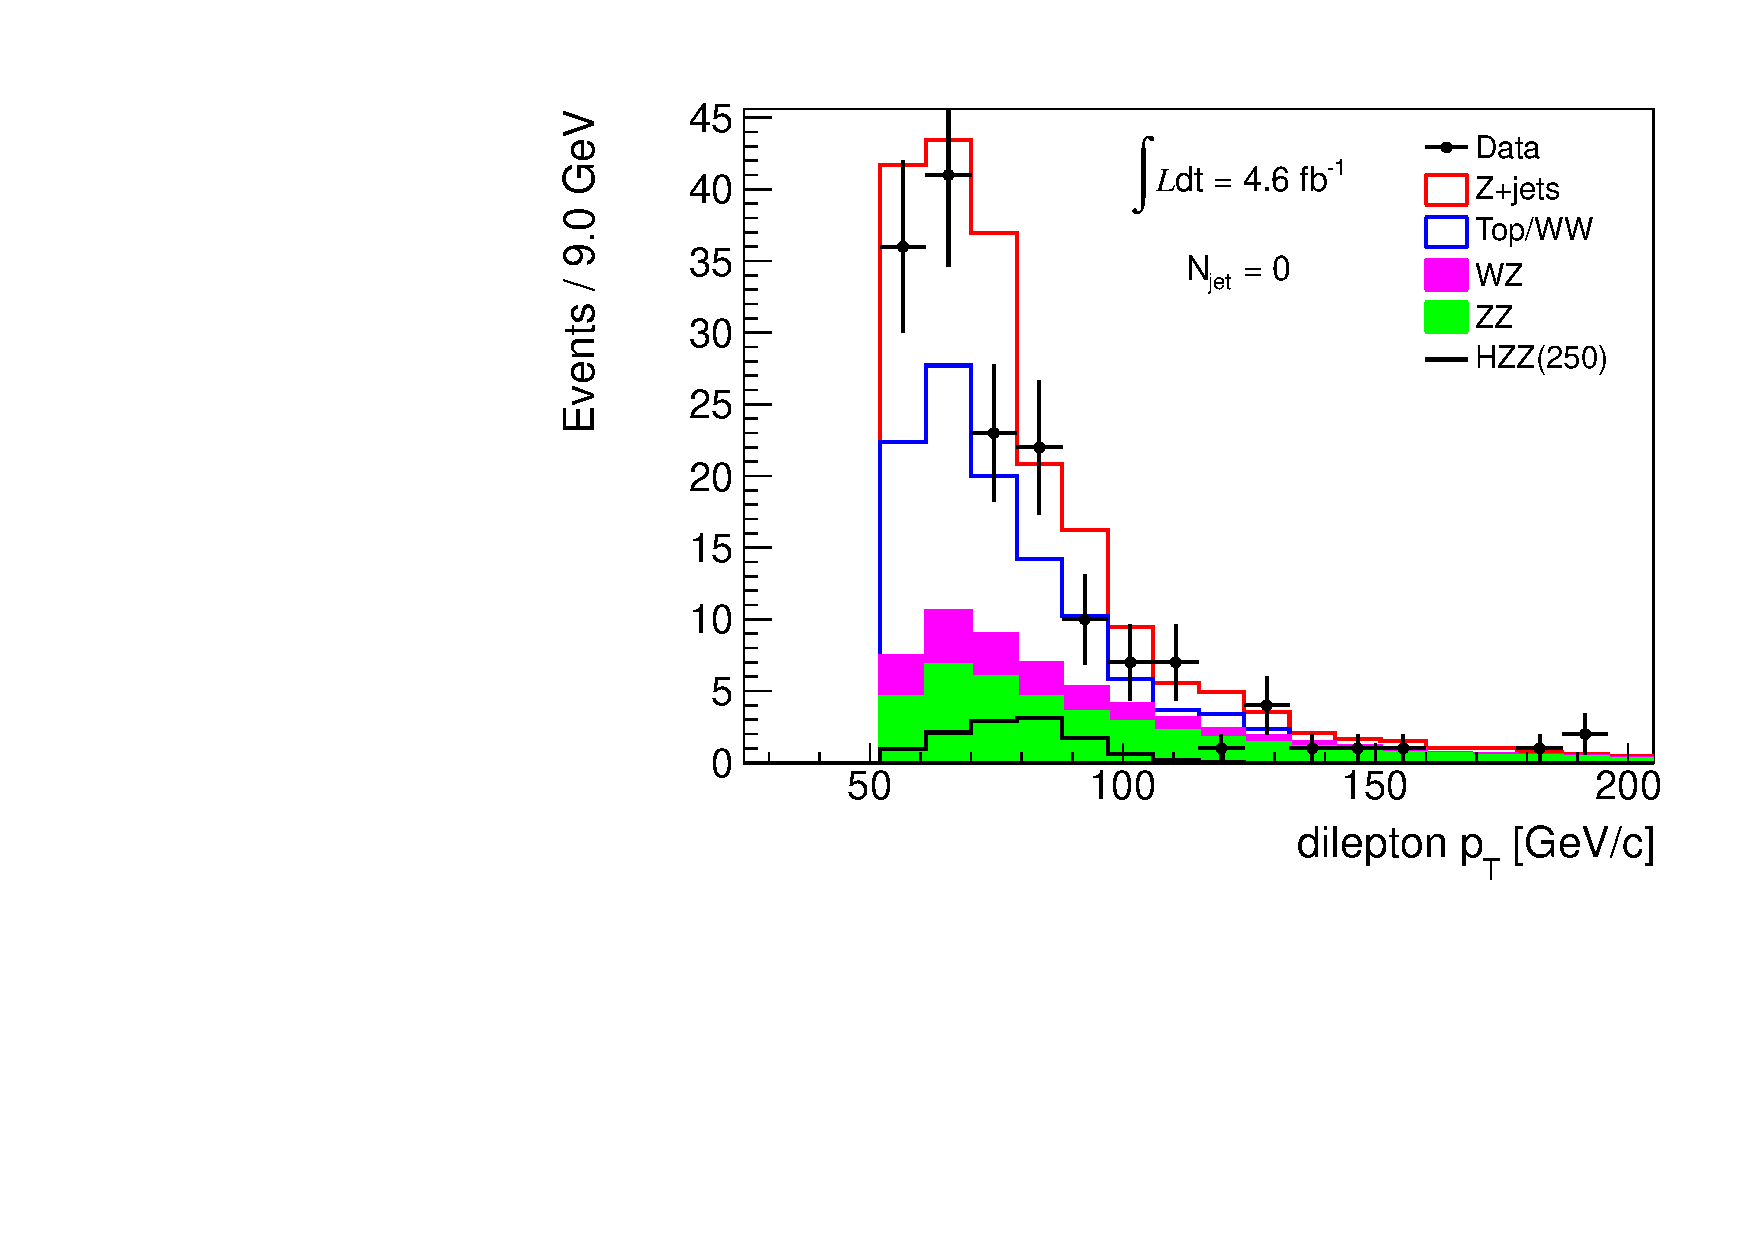
\includegraphics[width=.4\textwidth]{figures/presel_mH250_mm_dileppt_0j.pdf}} \\
\subfigure[1-Jet]{\label{subfig:zpt_mm_1j}
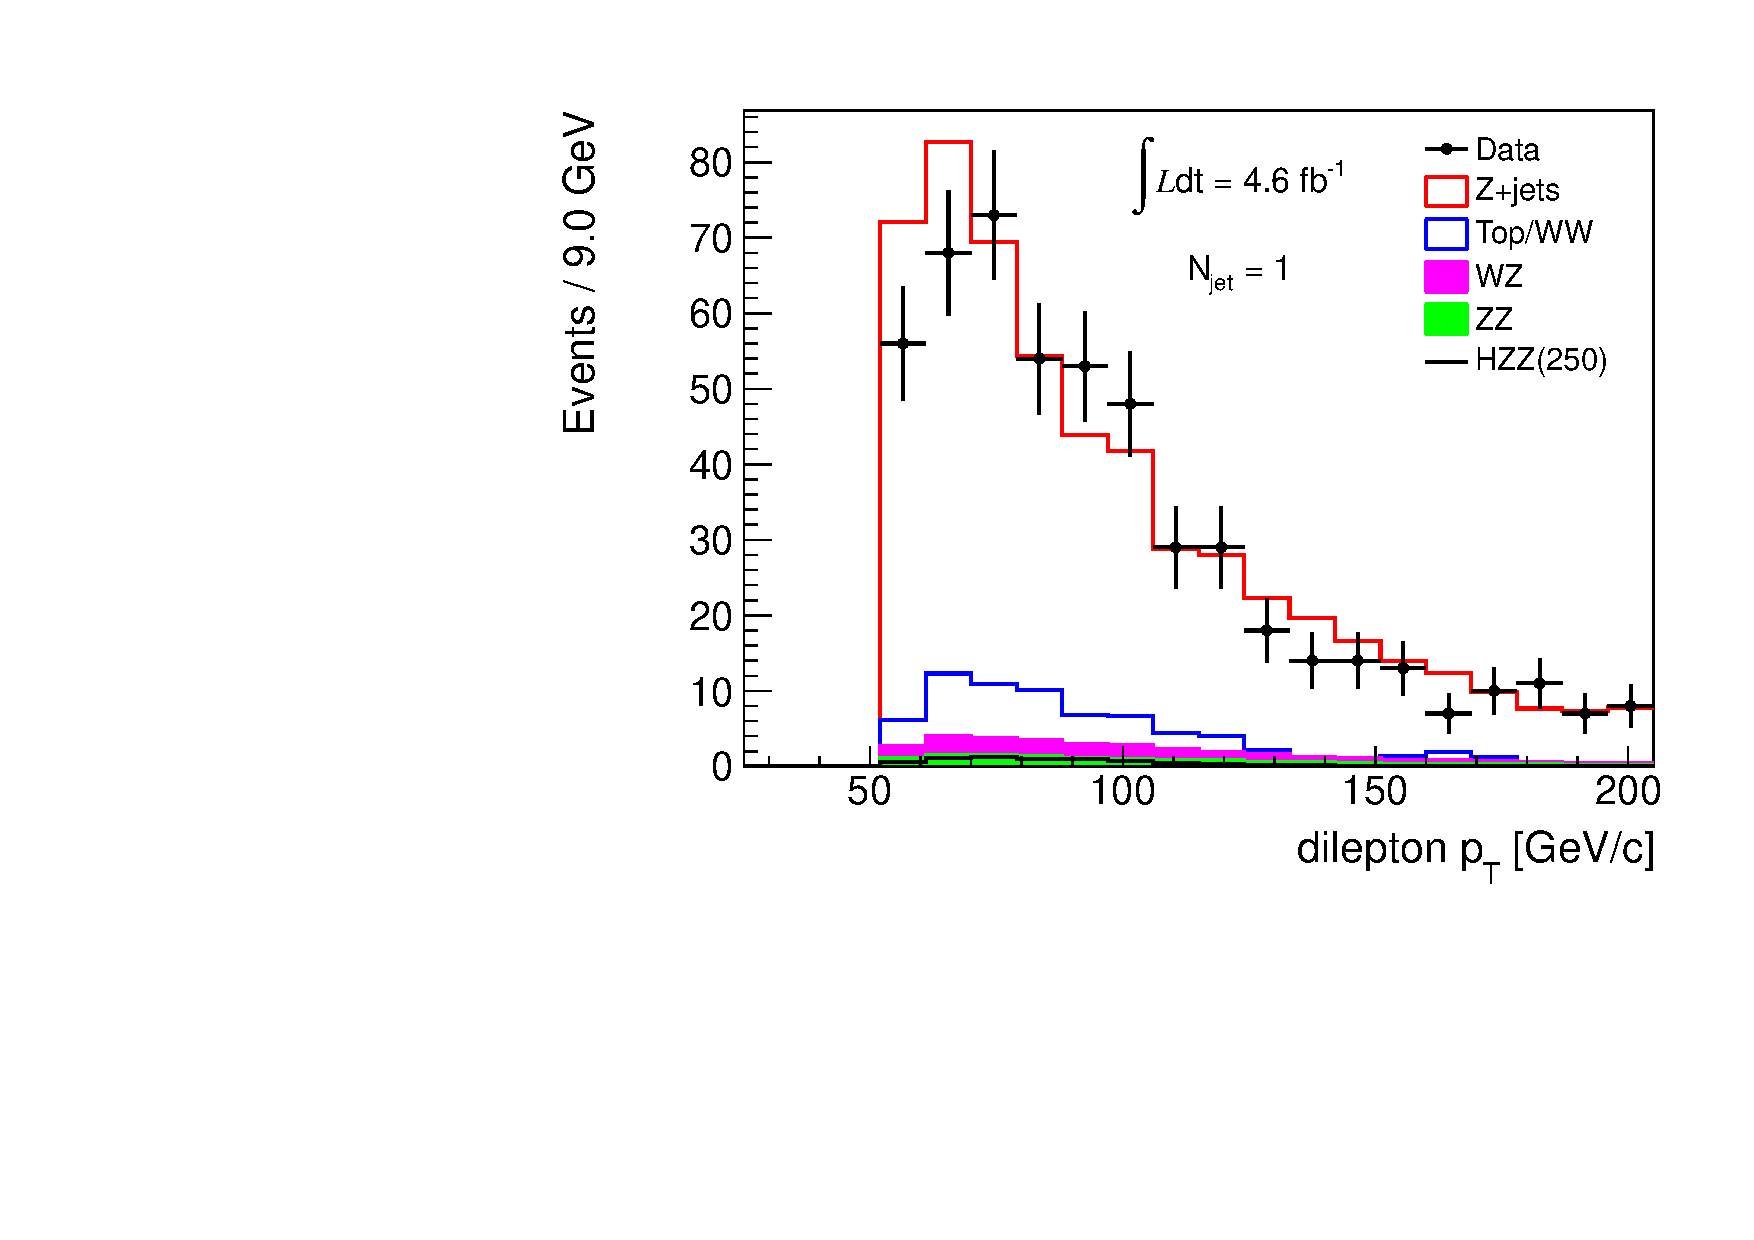
\includegraphics[width=.4\textwidth]{figures/presel_mH250_mm_dileppt_1j.pdf}}
\subfigure[$\geq$2 Jets]{\label{subfig:zpt_mm_2j}
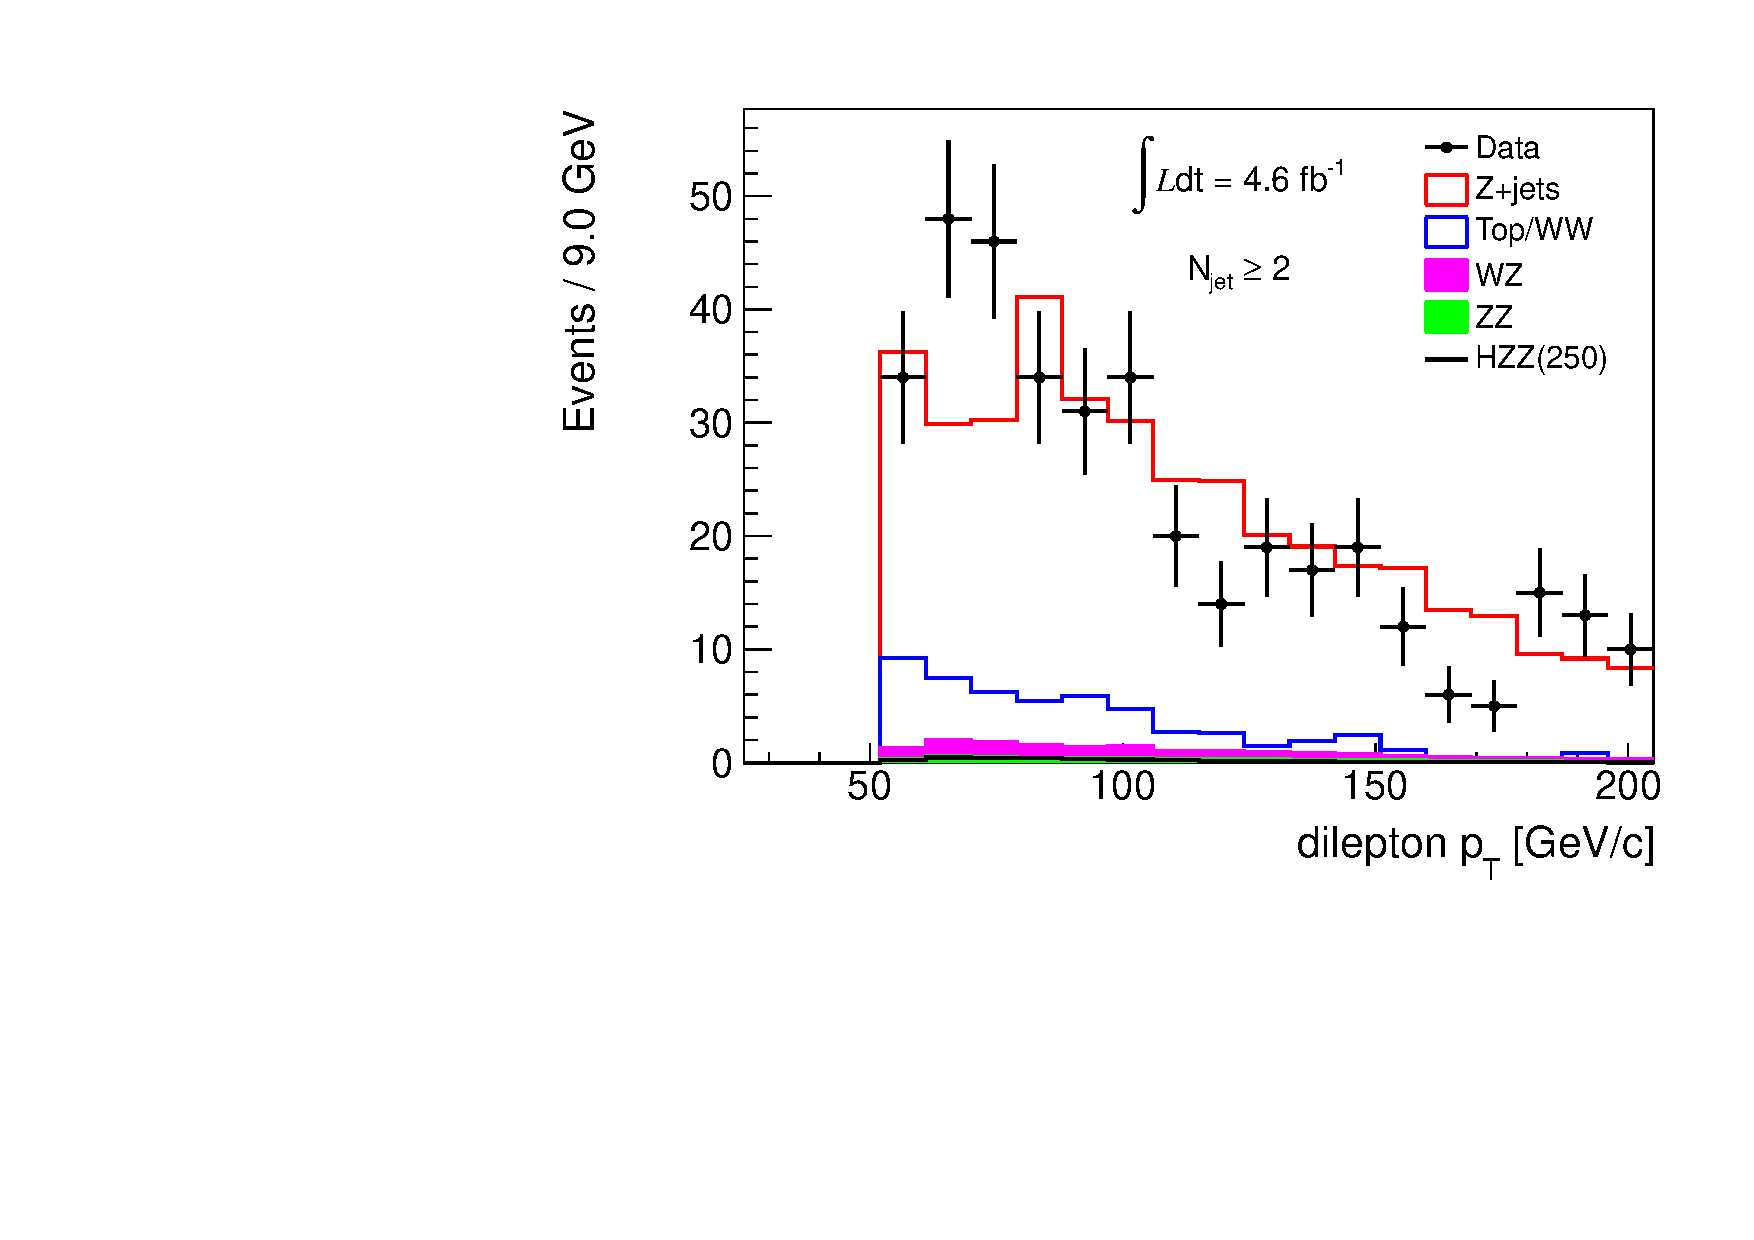
\includegraphics[width=.4\textwidth]{figures/presel_mH250_mm_dileppt_2j.pdf}}
\caption{Dilepton $p_T$ distribution in the muon channel after the $\ZZ$ preselection observed in data corresponding to $4.6$~\ifb data in 
the Inclusive~\subref{subfig:zpt_mm_incl}, 0-Jet~\subref{subfig:zpt_mm_0j}, 1-Jet~\subref{subfig:zpt_mm_1j} and $\geq$2-Jets~\subref{subfig:zpt_mm_2j} bins, 
compared to the expected from simulation for signal and background. The MC backgrounds are scaled as appropriate and the photon+jets estimate of the 
Z+jets background is added to the stack.}
\label{fig:zpt_zzpresel_mm}
\end{center}
\end{figure}
%%%%%%%%

%%%%%%%%
\begin{figure}[!hbtp]
\begin{center}
\subfigure[Inclusive]{\label{subfig:zpt_ee_incl}
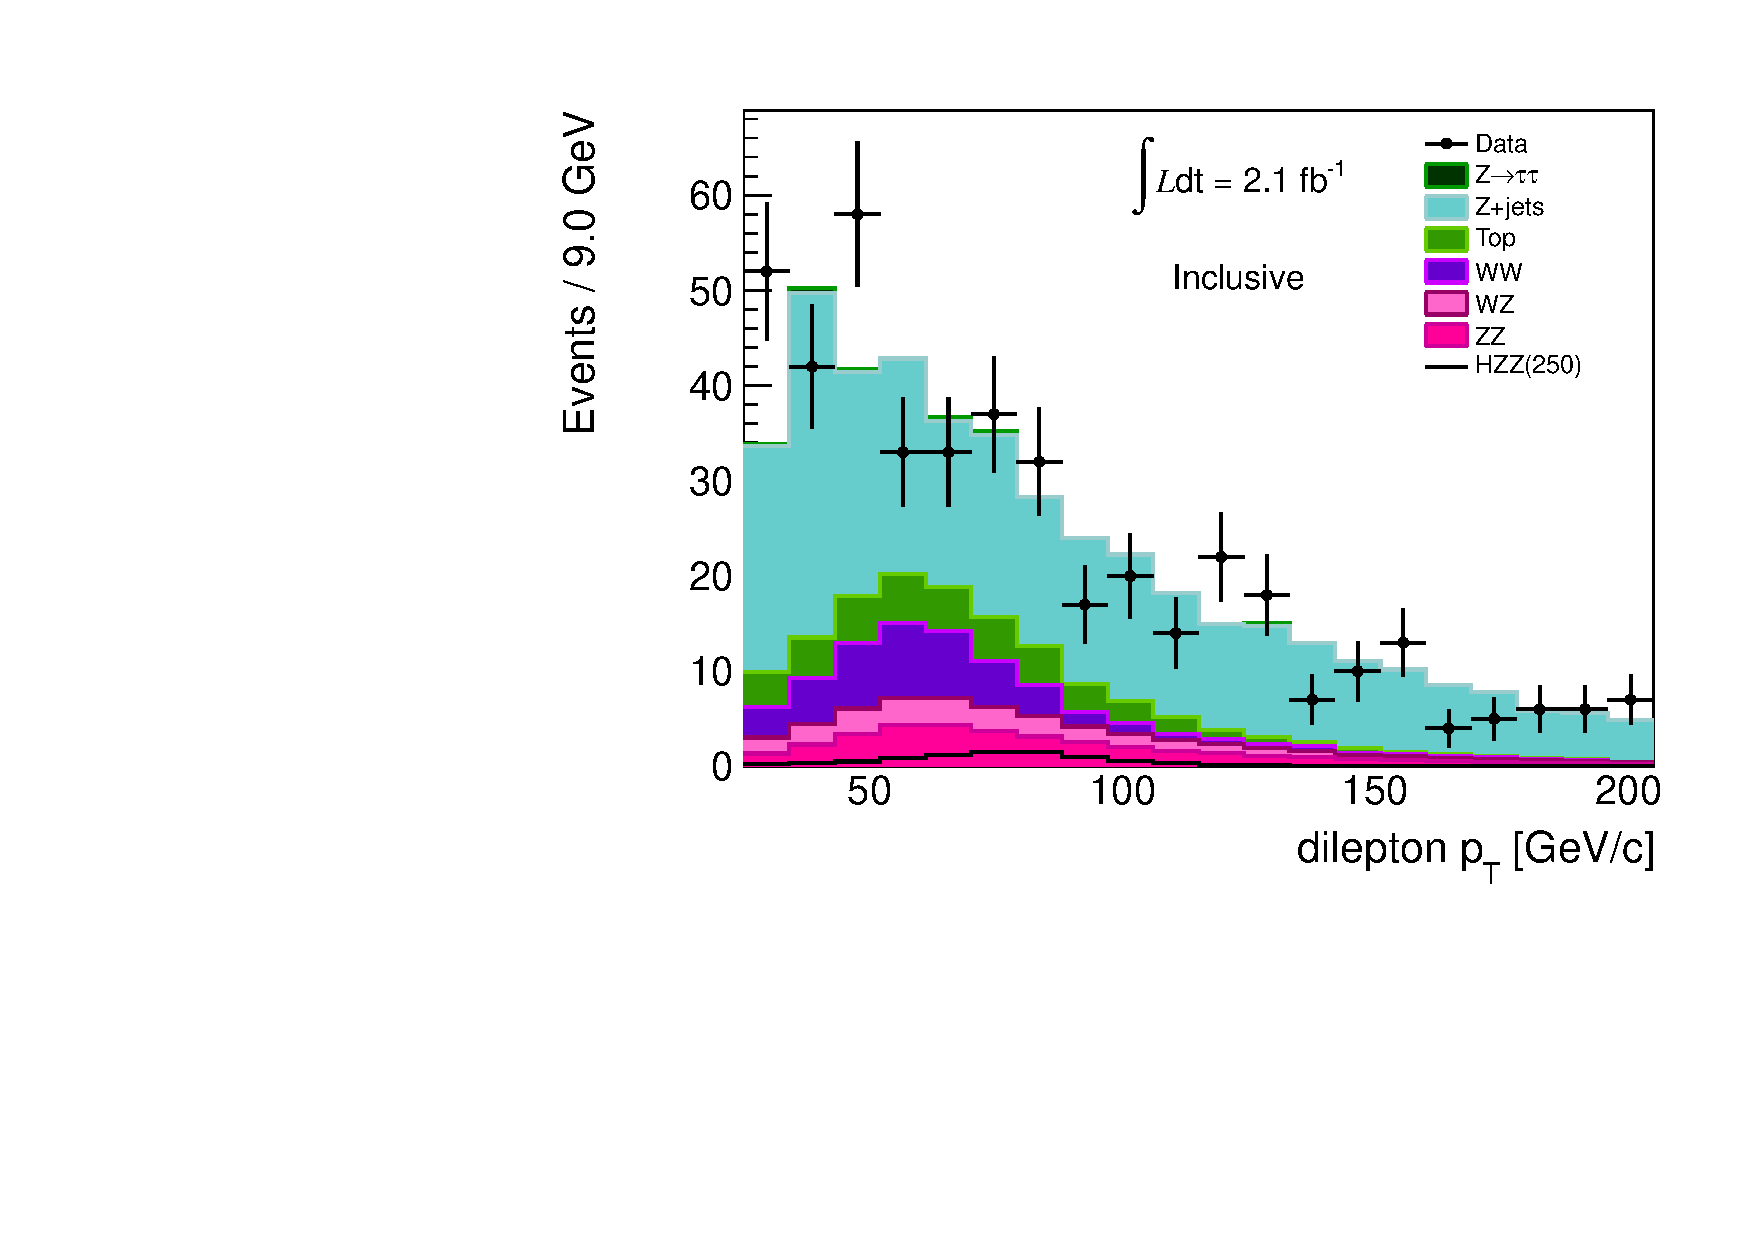
\includegraphics[width=.4\textwidth]{figures/presel_mH250_ee_dileppt_incl.pdf}}
\subfigure[0-Jet]{\label{subfig:zpt_ee_0j}
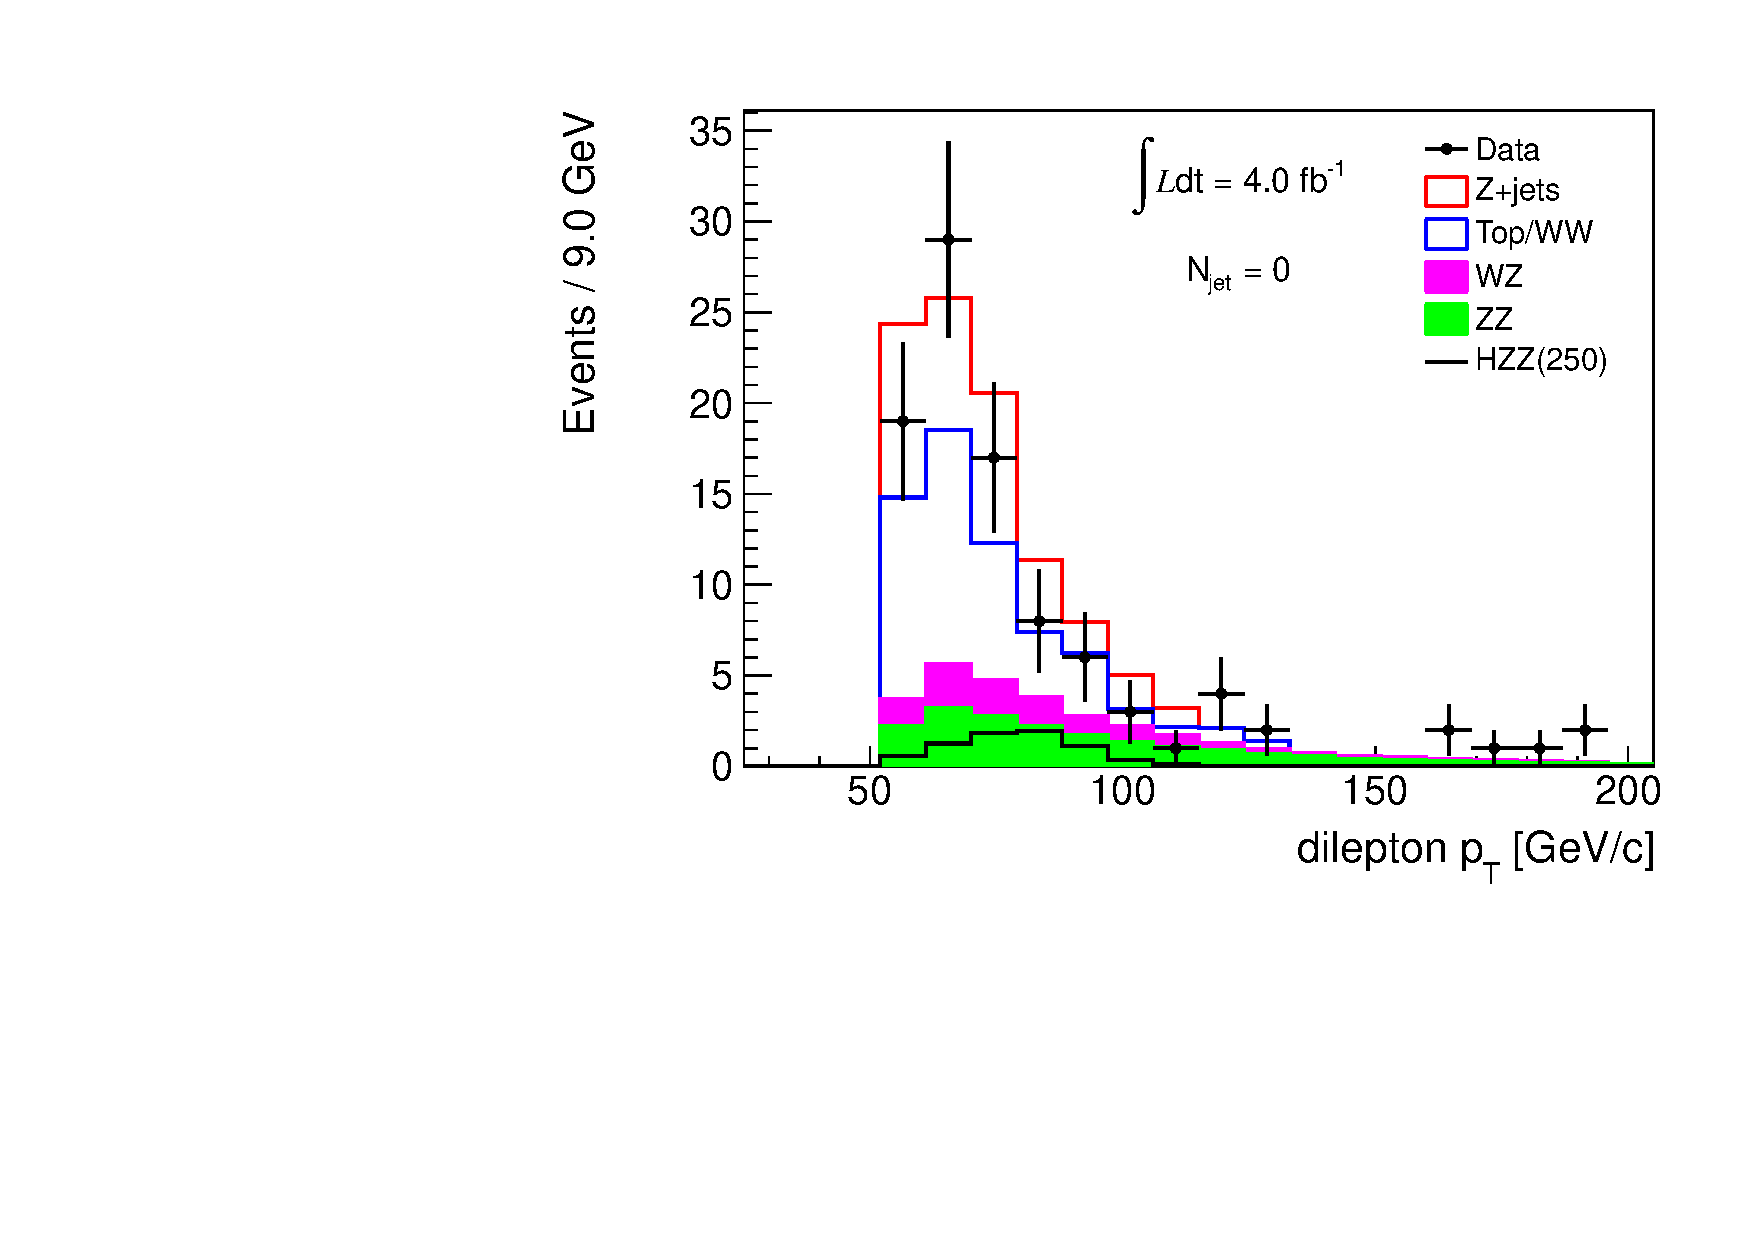
\includegraphics[width=.4\textwidth]{figures/presel_mH250_ee_dileppt_0j.pdf}} \\
\subfigure[1-Jet]{\label{subfig:zpt_ee_1j}
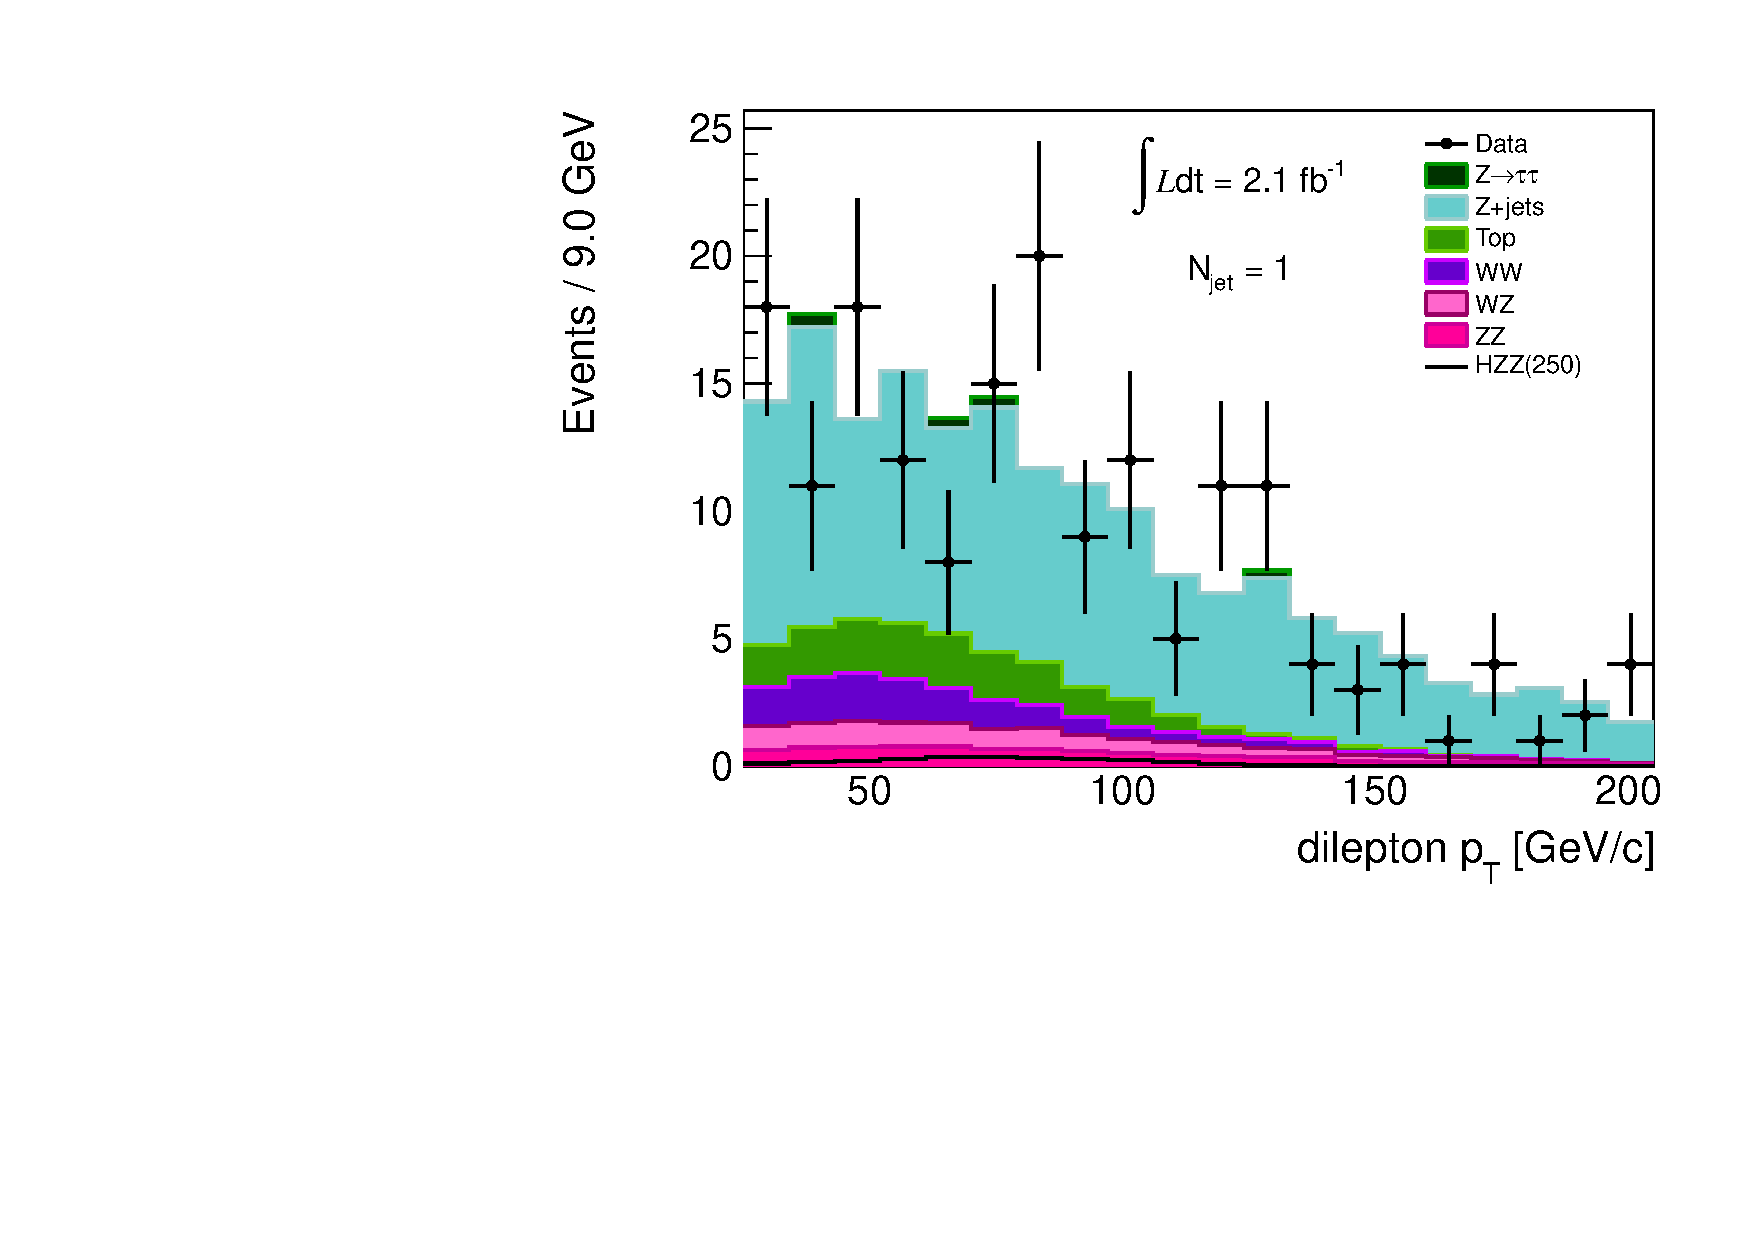
\includegraphics[width=.4\textwidth]{figures/presel_mH250_ee_dileppt_1j.pdf}}
\subfigure[$\geq$2 Jets]{\label{subfig:zpt_ee_2j}
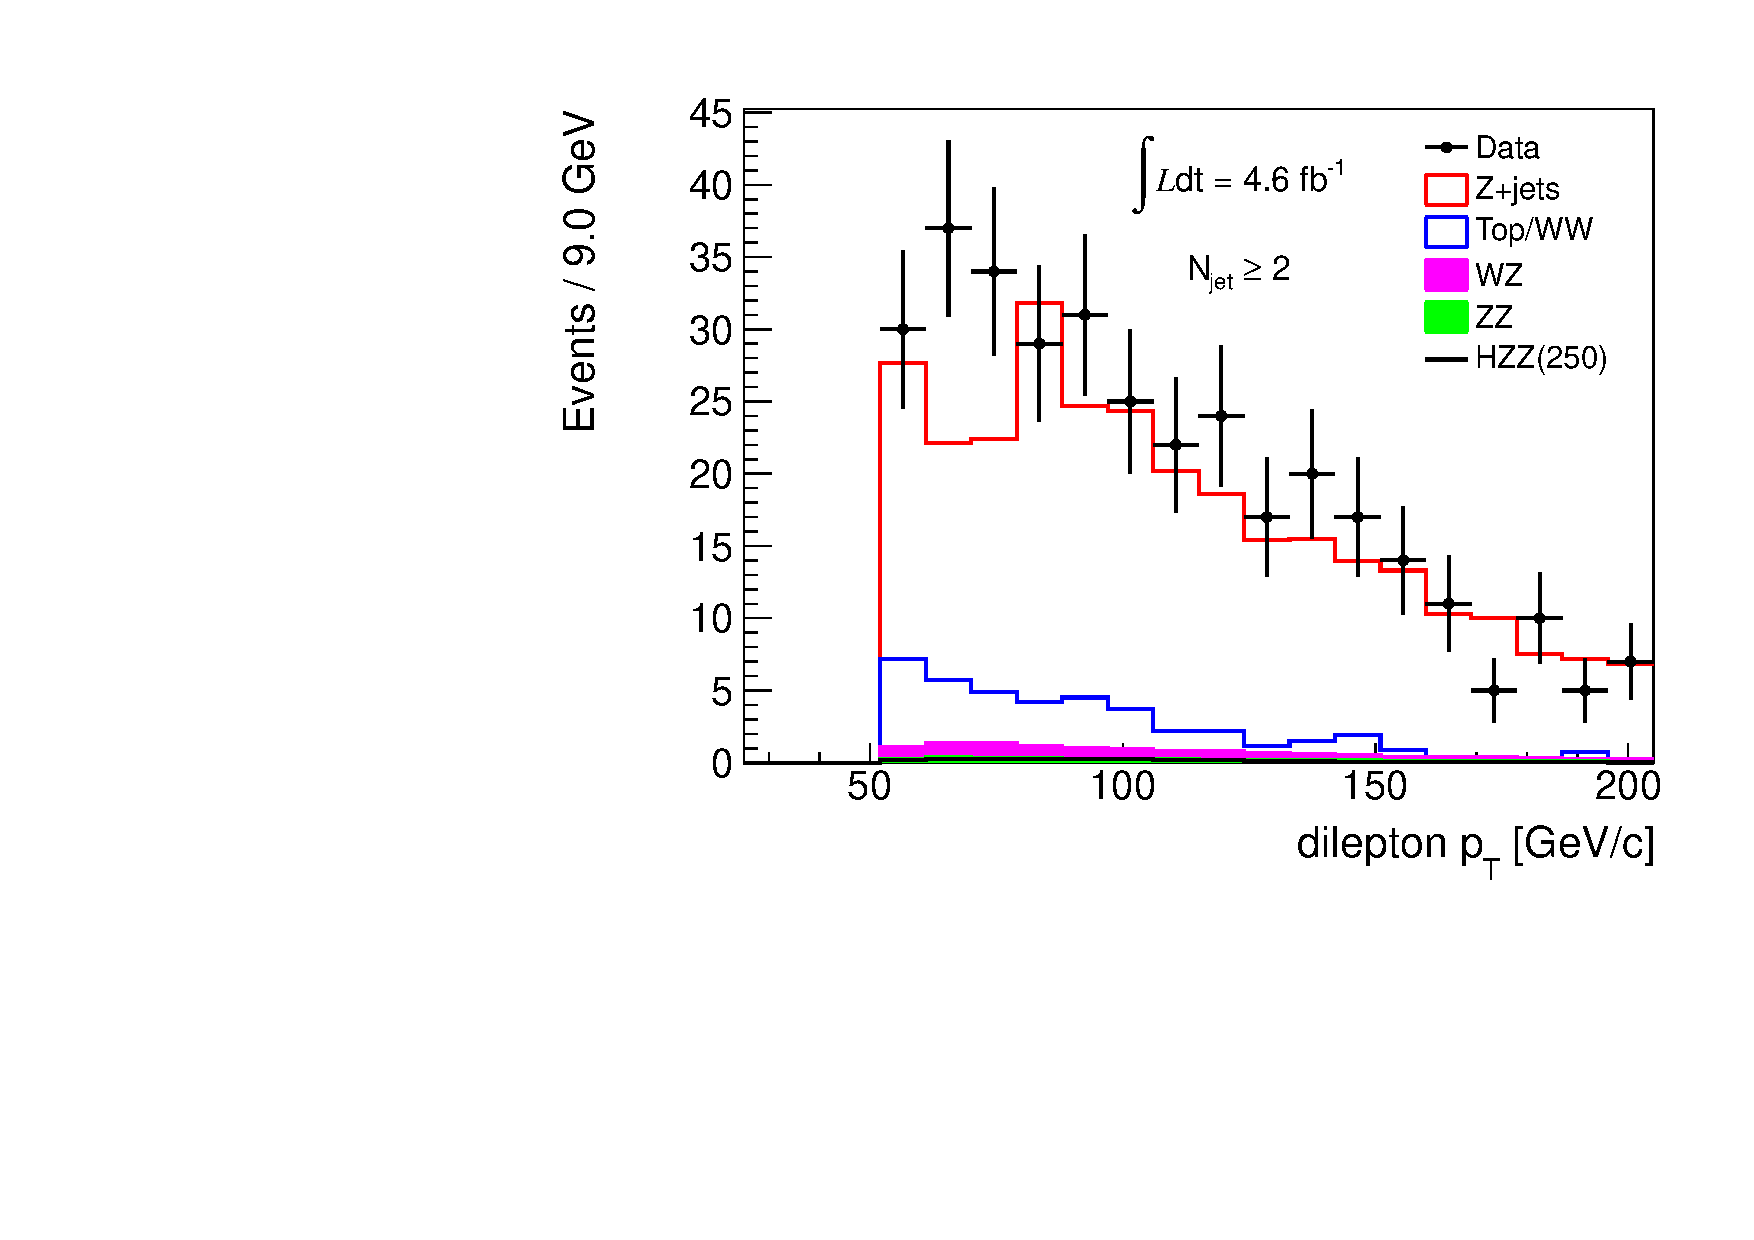
\includegraphics[width=.4\textwidth]{figures/presel_mH250_ee_dileppt_2j.pdf}}
\caption{Dilepton $p_T$ distribution in the electron channel after the $\ZZ$ preselection observed in data corresponding to $4.6$~\ifb data in 
the Inclusive~\subref{subfig:zpt_ee_incl}, 0-Jet~\subref{subfig:zpt_ee_0j}, 1-Jet~\subref{subfig:zpt_ee_1j} and $\geq$2-Jets~\subref{subfig:zpt_ee_2j} bins, 
compared to the expected from simulation for signal and background. The MC backgrounds are scaled as appropriate and the photon+jets estimate of the 
Z+jets background is added to the stack.}
\label{fig:zpt_zzpresel_ee}
\end{center}
\end{figure}
%%%%%%%%

%%%%%%%%
\begin{figure}[!hbtp]
\begin{center}
\subfigure[Inclusive]{\label{subfig:met_mm_incl}
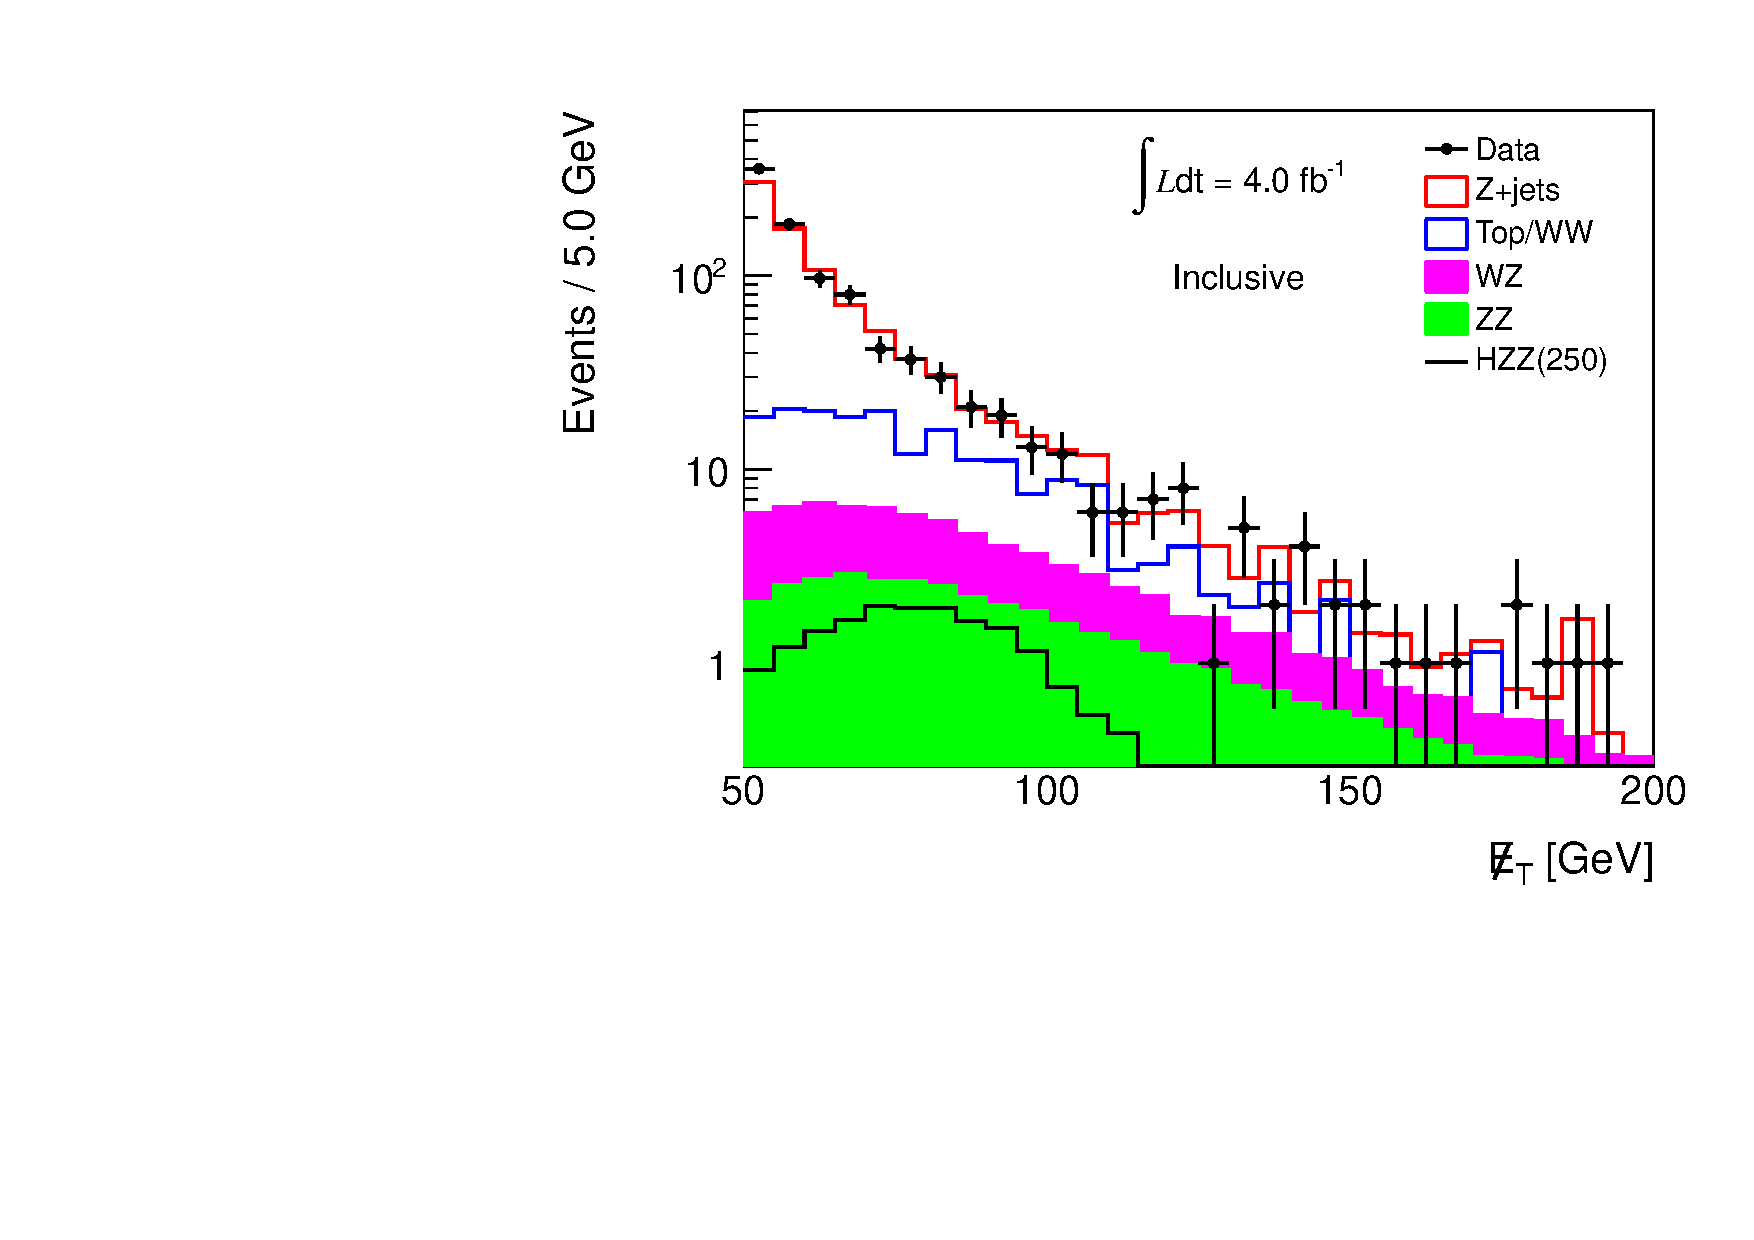
\includegraphics[width=.4\textwidth]{figures/presel_mH250_mm_metlog_incl.pdf}}
\subfigure[0-Jet]{\label{subfig:met_mm_0j}
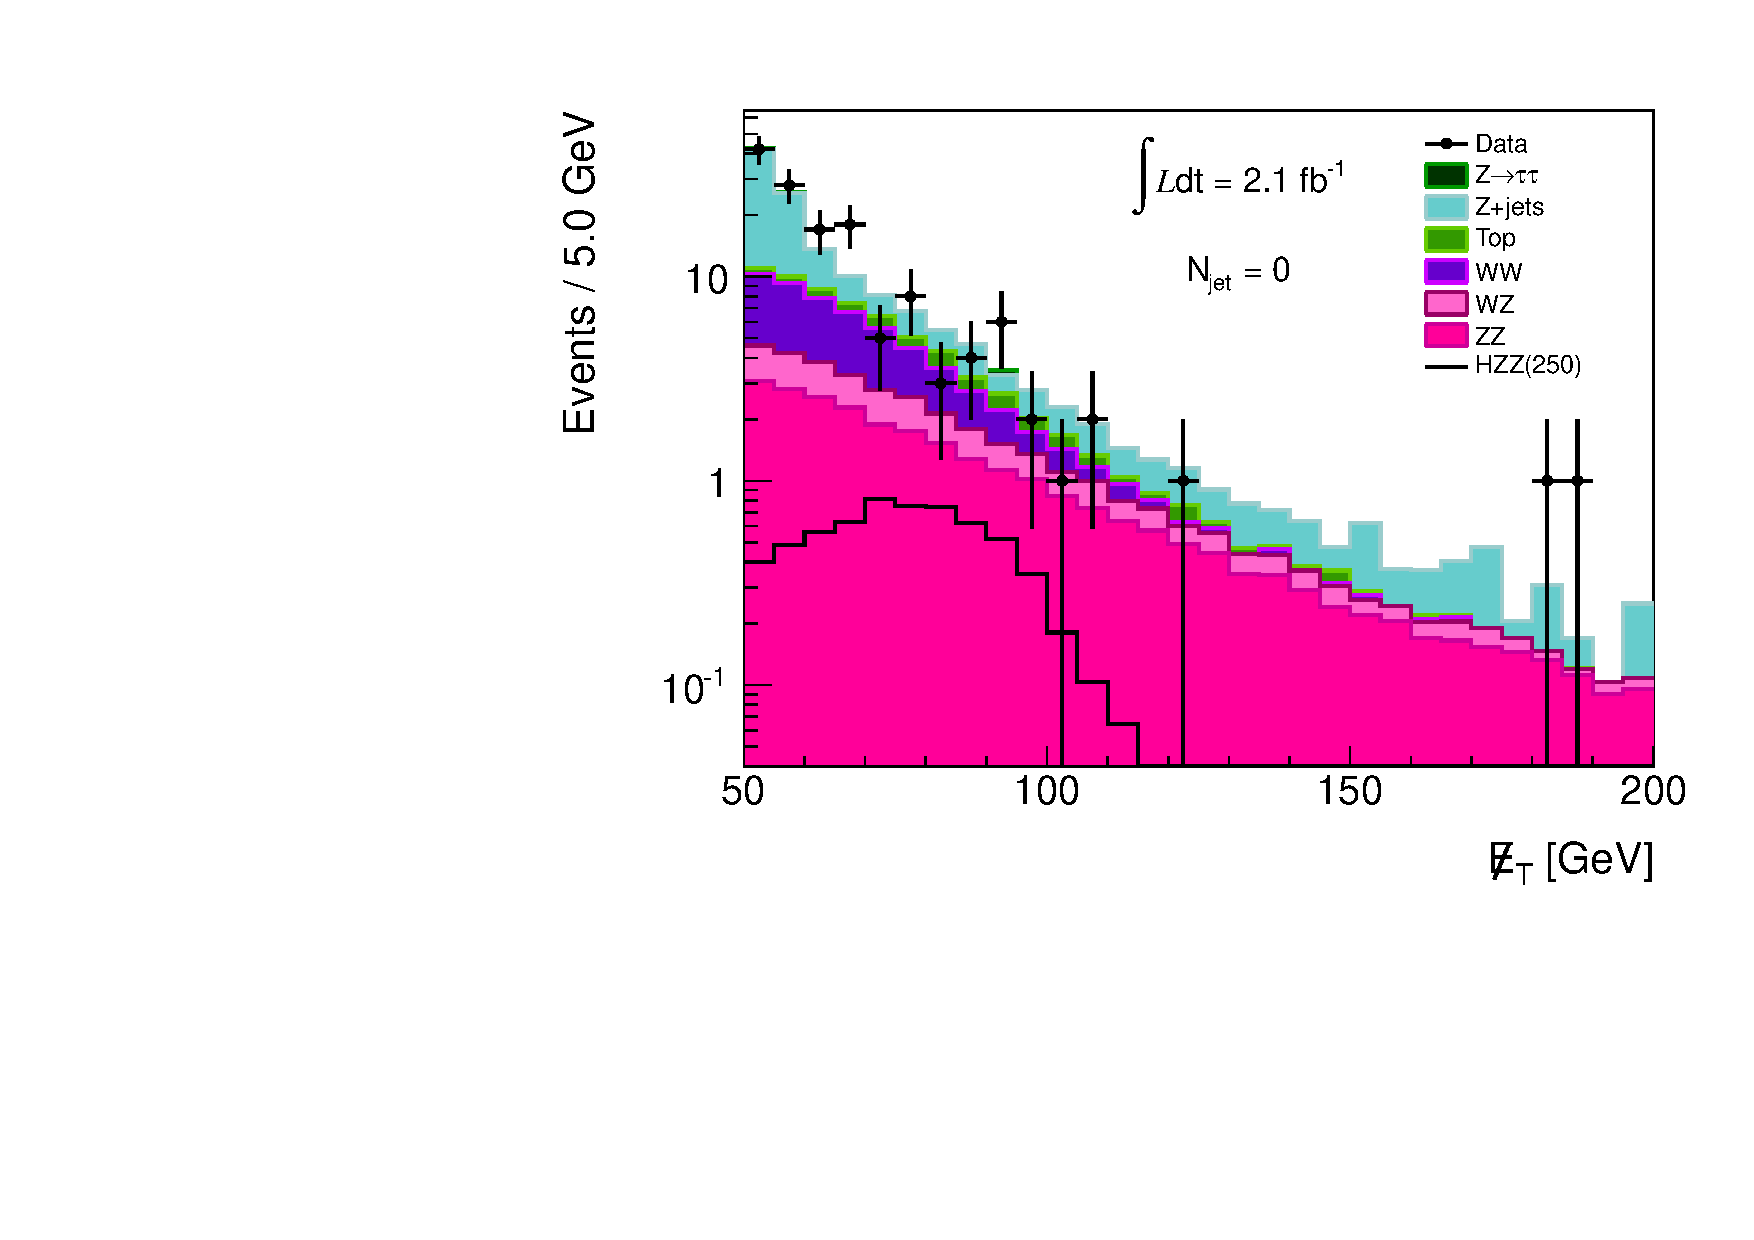
\includegraphics[width=.4\textwidth]{figures/presel_mH250_mm_metlog_0j.pdf}} \\
\subfigure[1-Jet]{\label{subfig:met_mm_1j}
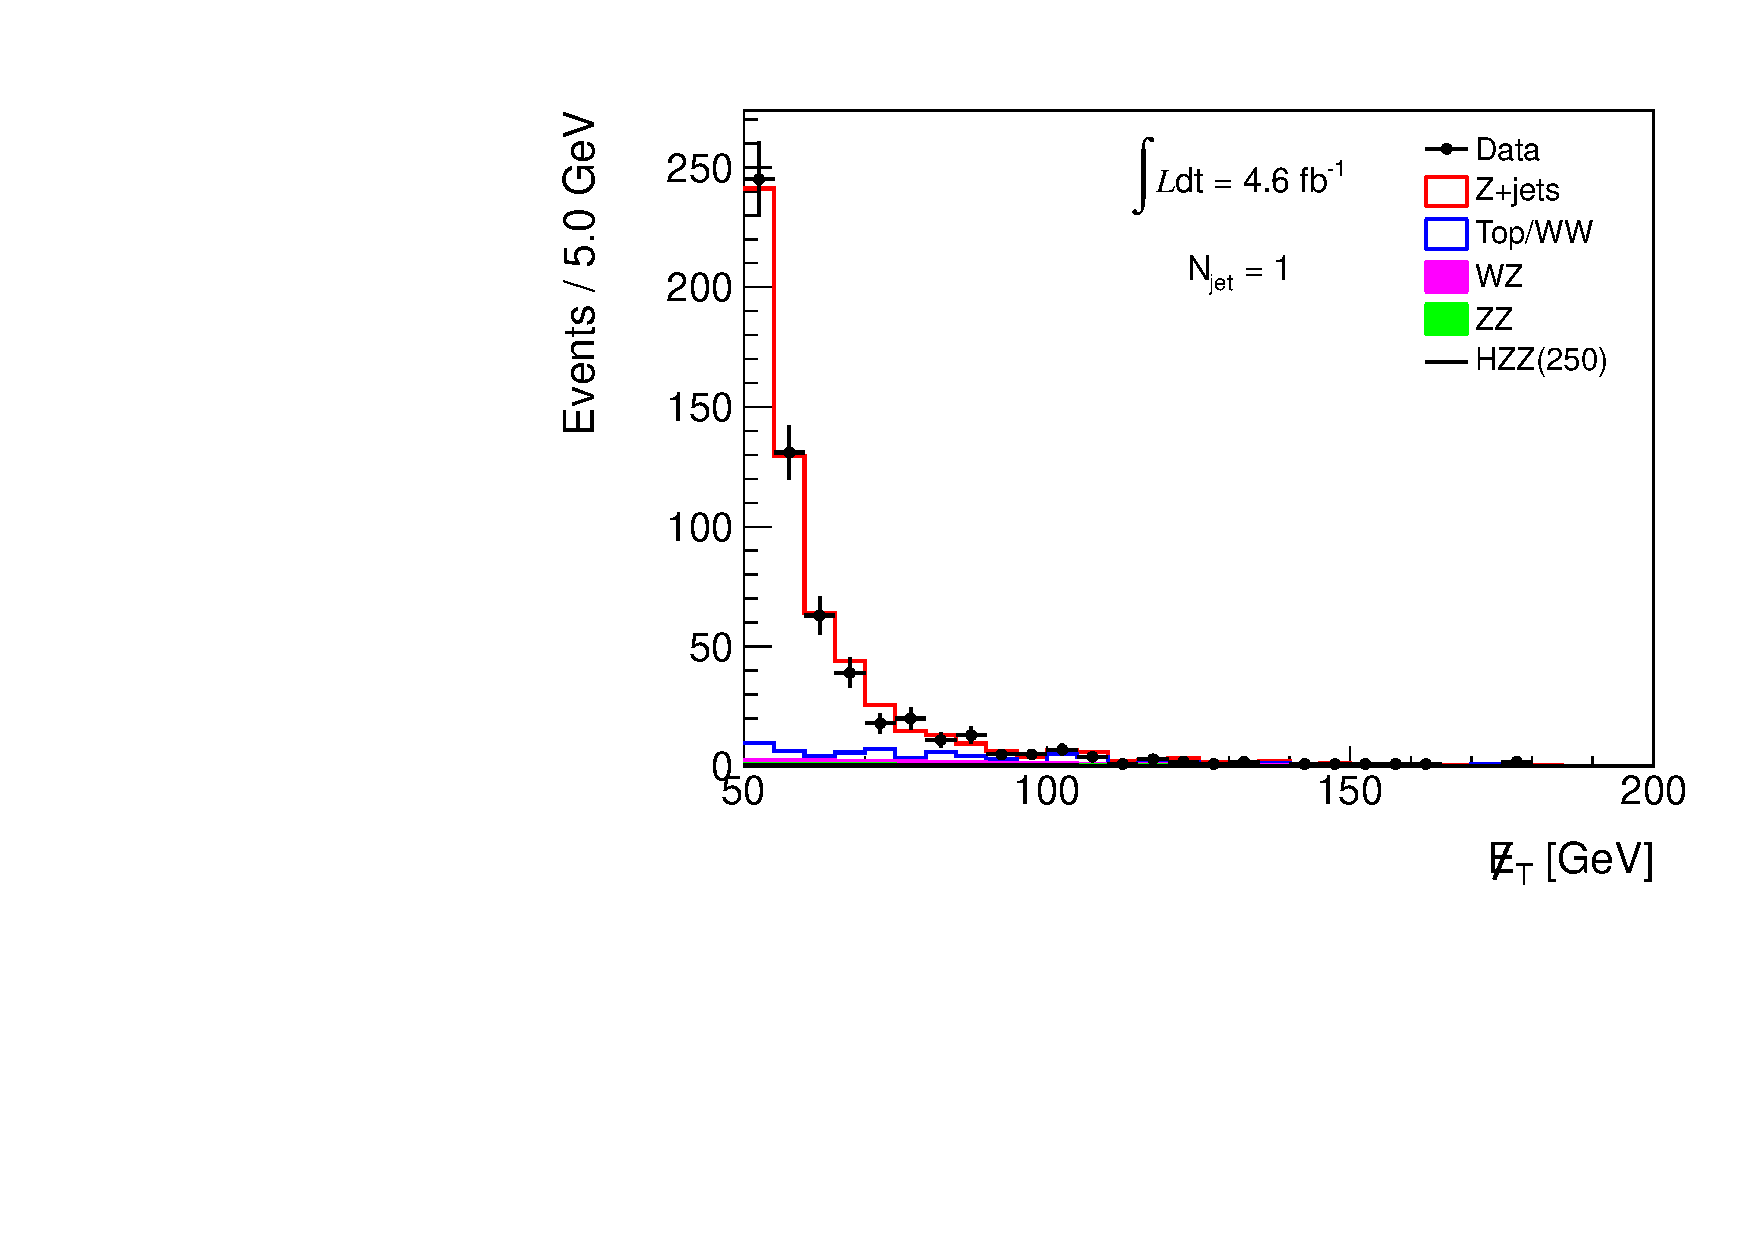
\includegraphics[width=.4\textwidth]{figures/presel_mH250_mm_metlog_1j.pdf}}
\subfigure[$\geq$2 Jets]{\label{subfig:met_mm_2j}
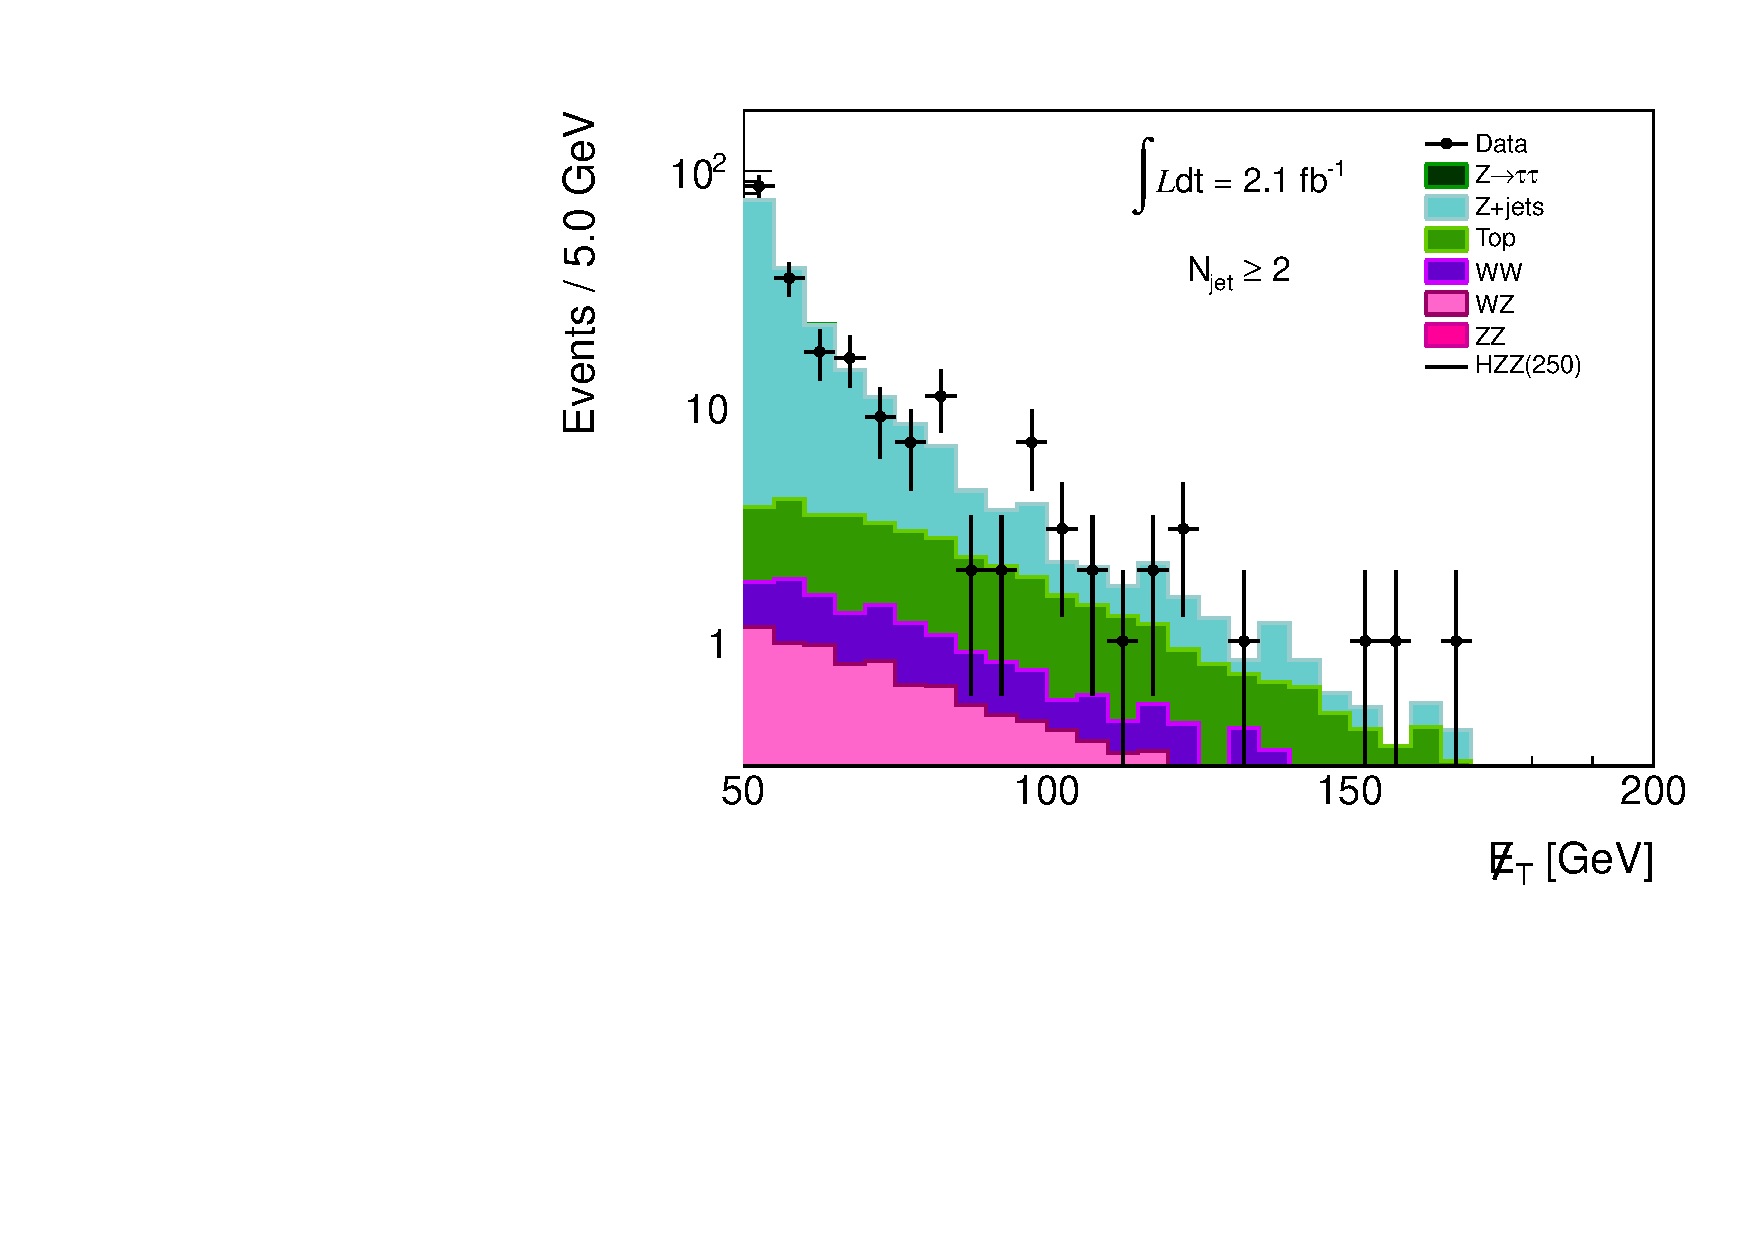
\includegraphics[width=.4\textwidth]{figures/presel_mH250_mm_metlog_2j.pdf}}
\caption{Missing transverse energy distribution in the muon channel after the $\ZZ$ preselection observed in data corresponding to $4.6$~\ifb data in 
the Inclusive~\subref{subfig:met_mm_incl}, 0-Jet~\subref{subfig:met_mm_0j}, 1-Jet~\subref{subfig:met_mm_1j} and $\geq$2-Jets~\subref{subfig:met_mm_2j} bins, 
compared to the expected from simulation for signal and background. The MC backgrounds are scaled as appropriate and the photon+jets estimate of the 
Z+jets background is added to the stack.}
\label{fig:met_zzpresel_mm}
\end{center}
\end{figure}
%%%%%%%%

%%%%%%%%
\begin{figure}[!hbtp]
\begin{center}
\subfigure[Inclusive]{\label{subfig:met_ee_incl}
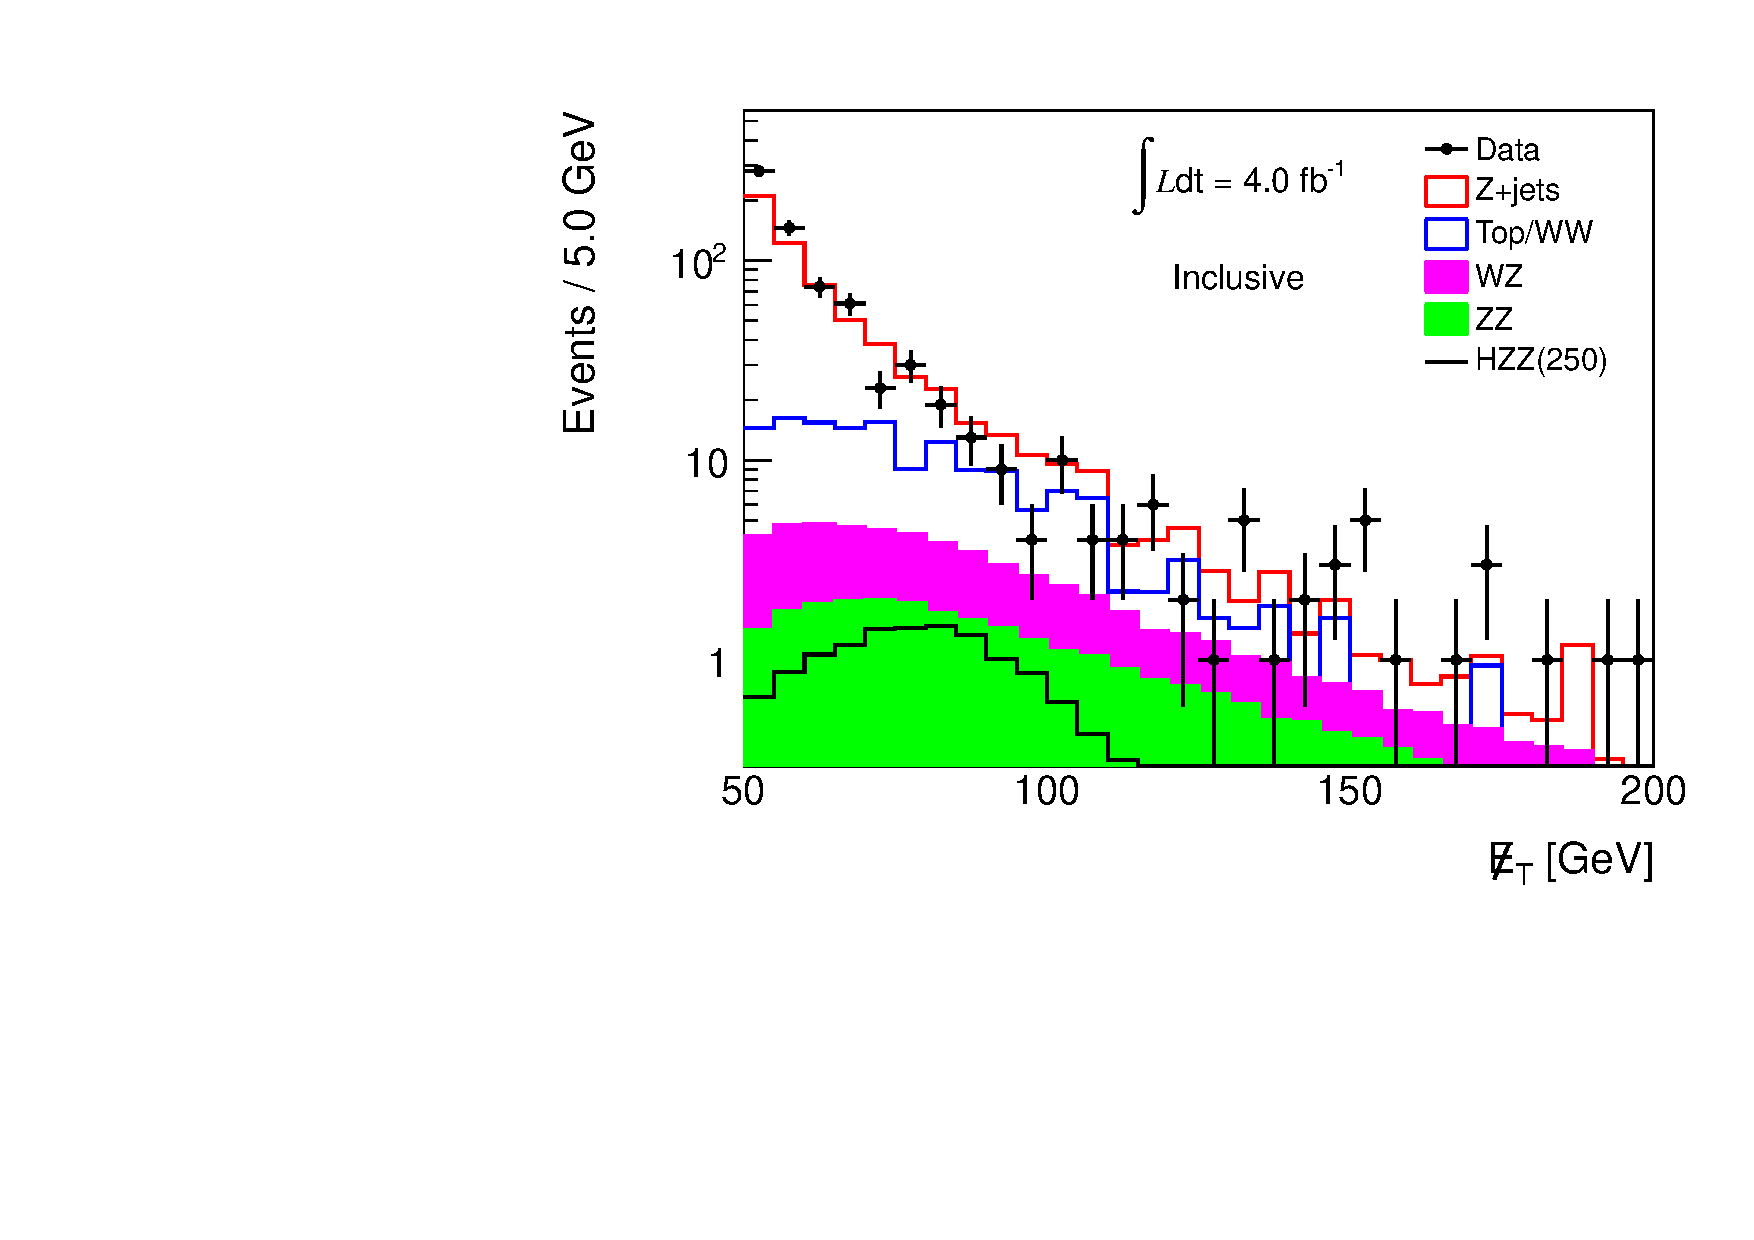
\includegraphics[width=.4\textwidth]{figures/presel_mH250_ee_metlog_incl.pdf}}
\subfigure[0-Jet]{\label{subfig:met_ee_0j}
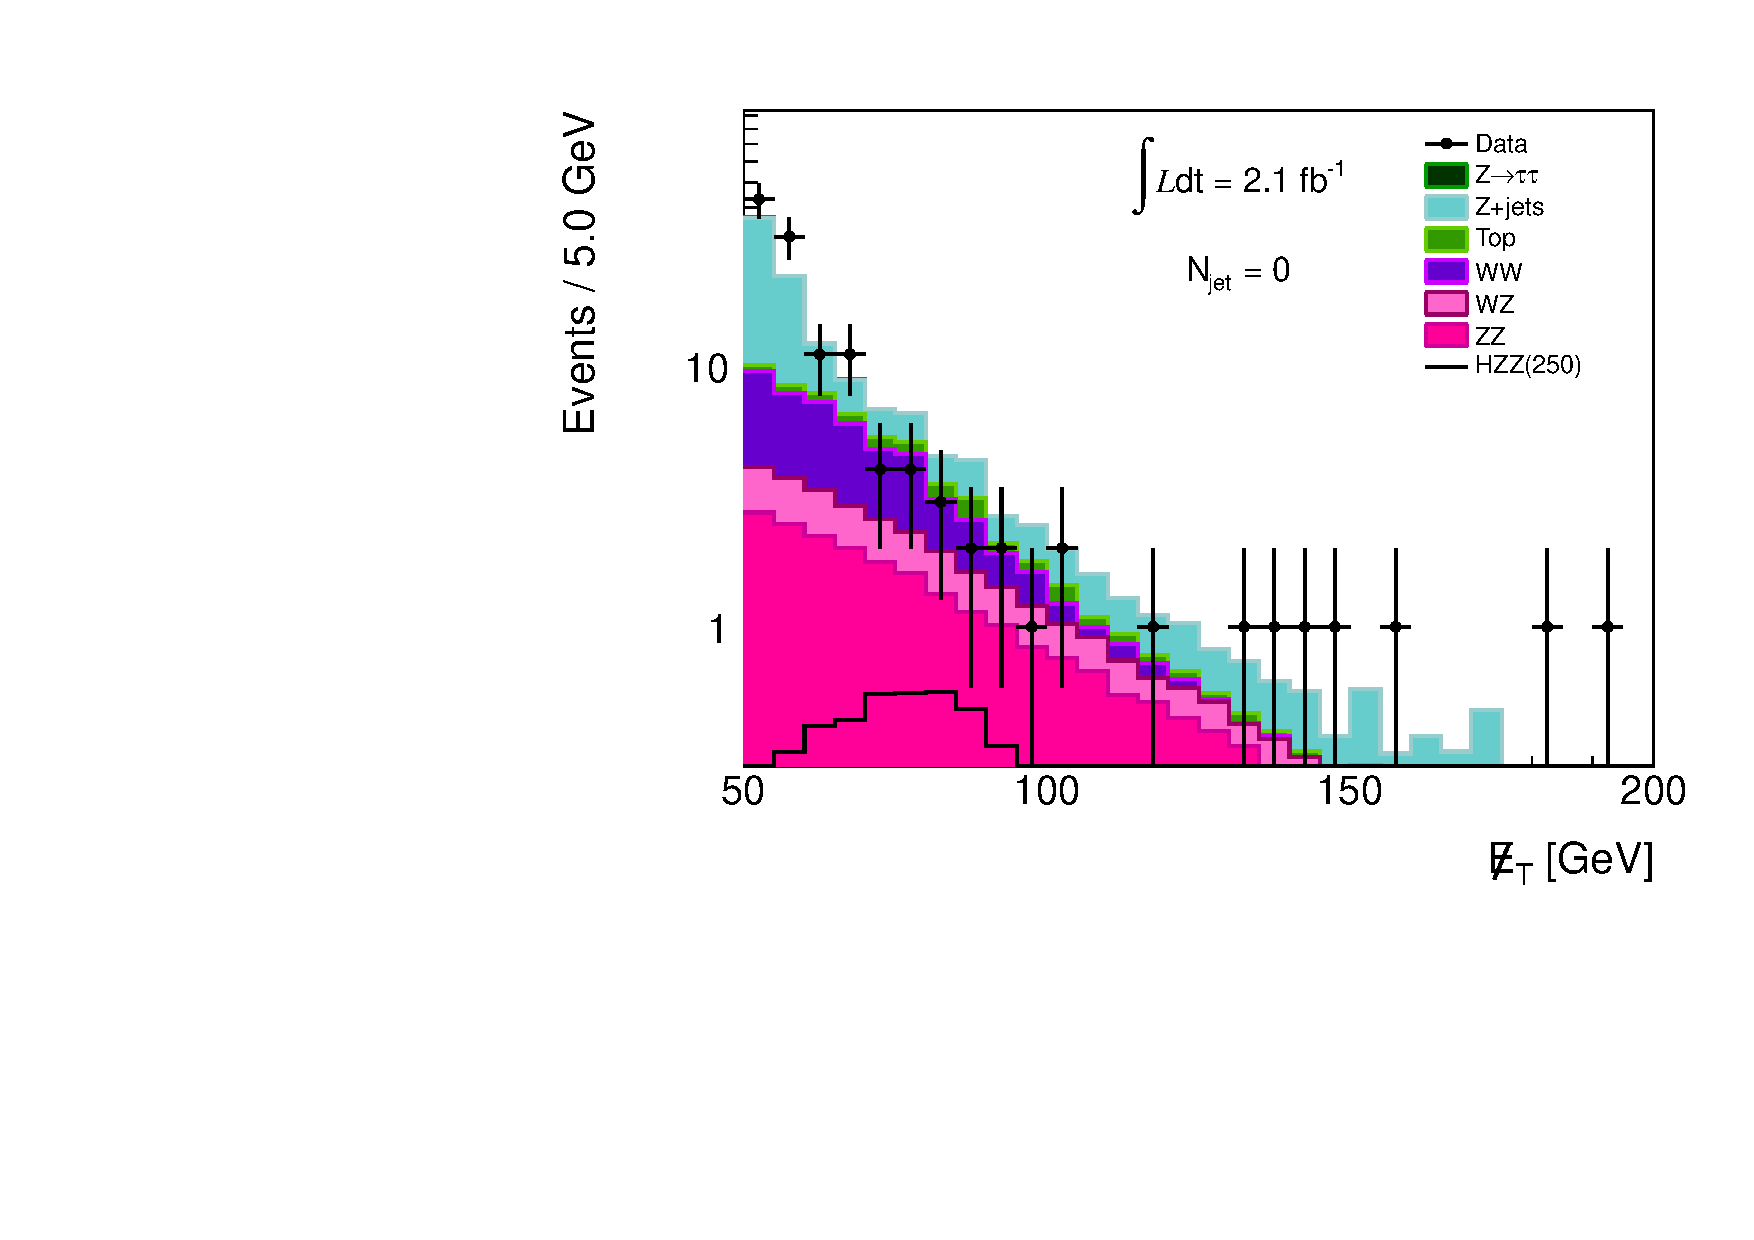
\includegraphics[width=.4\textwidth]{figures/presel_mH250_ee_metlog_0j.pdf}} \\
\subfigure[1-Jet]{\label{subfig:met_ee_1j}
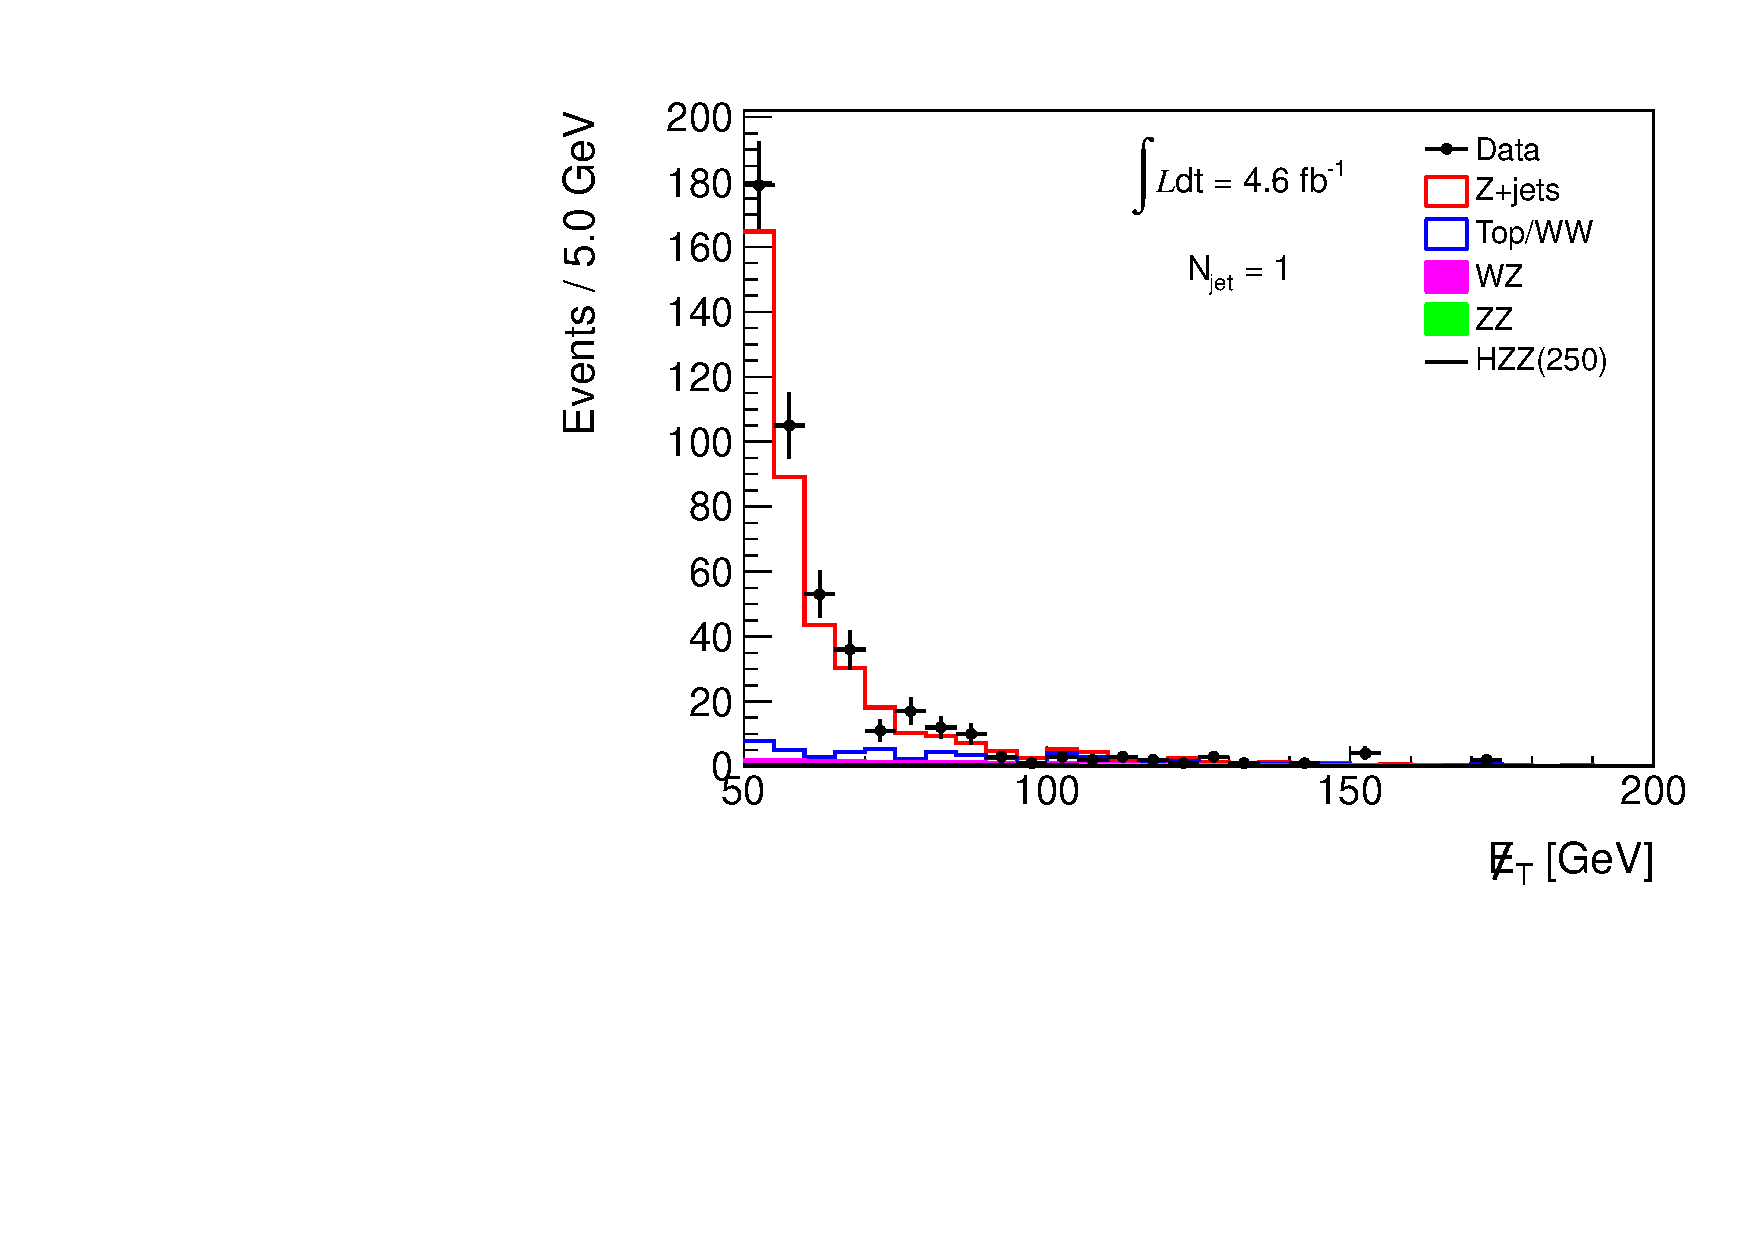
\includegraphics[width=.4\textwidth]{figures/presel_mH250_ee_metlog_1j.pdf}}
\subfigure[$\geq$2 Jets]{\label{subfig:met_ee_2j}
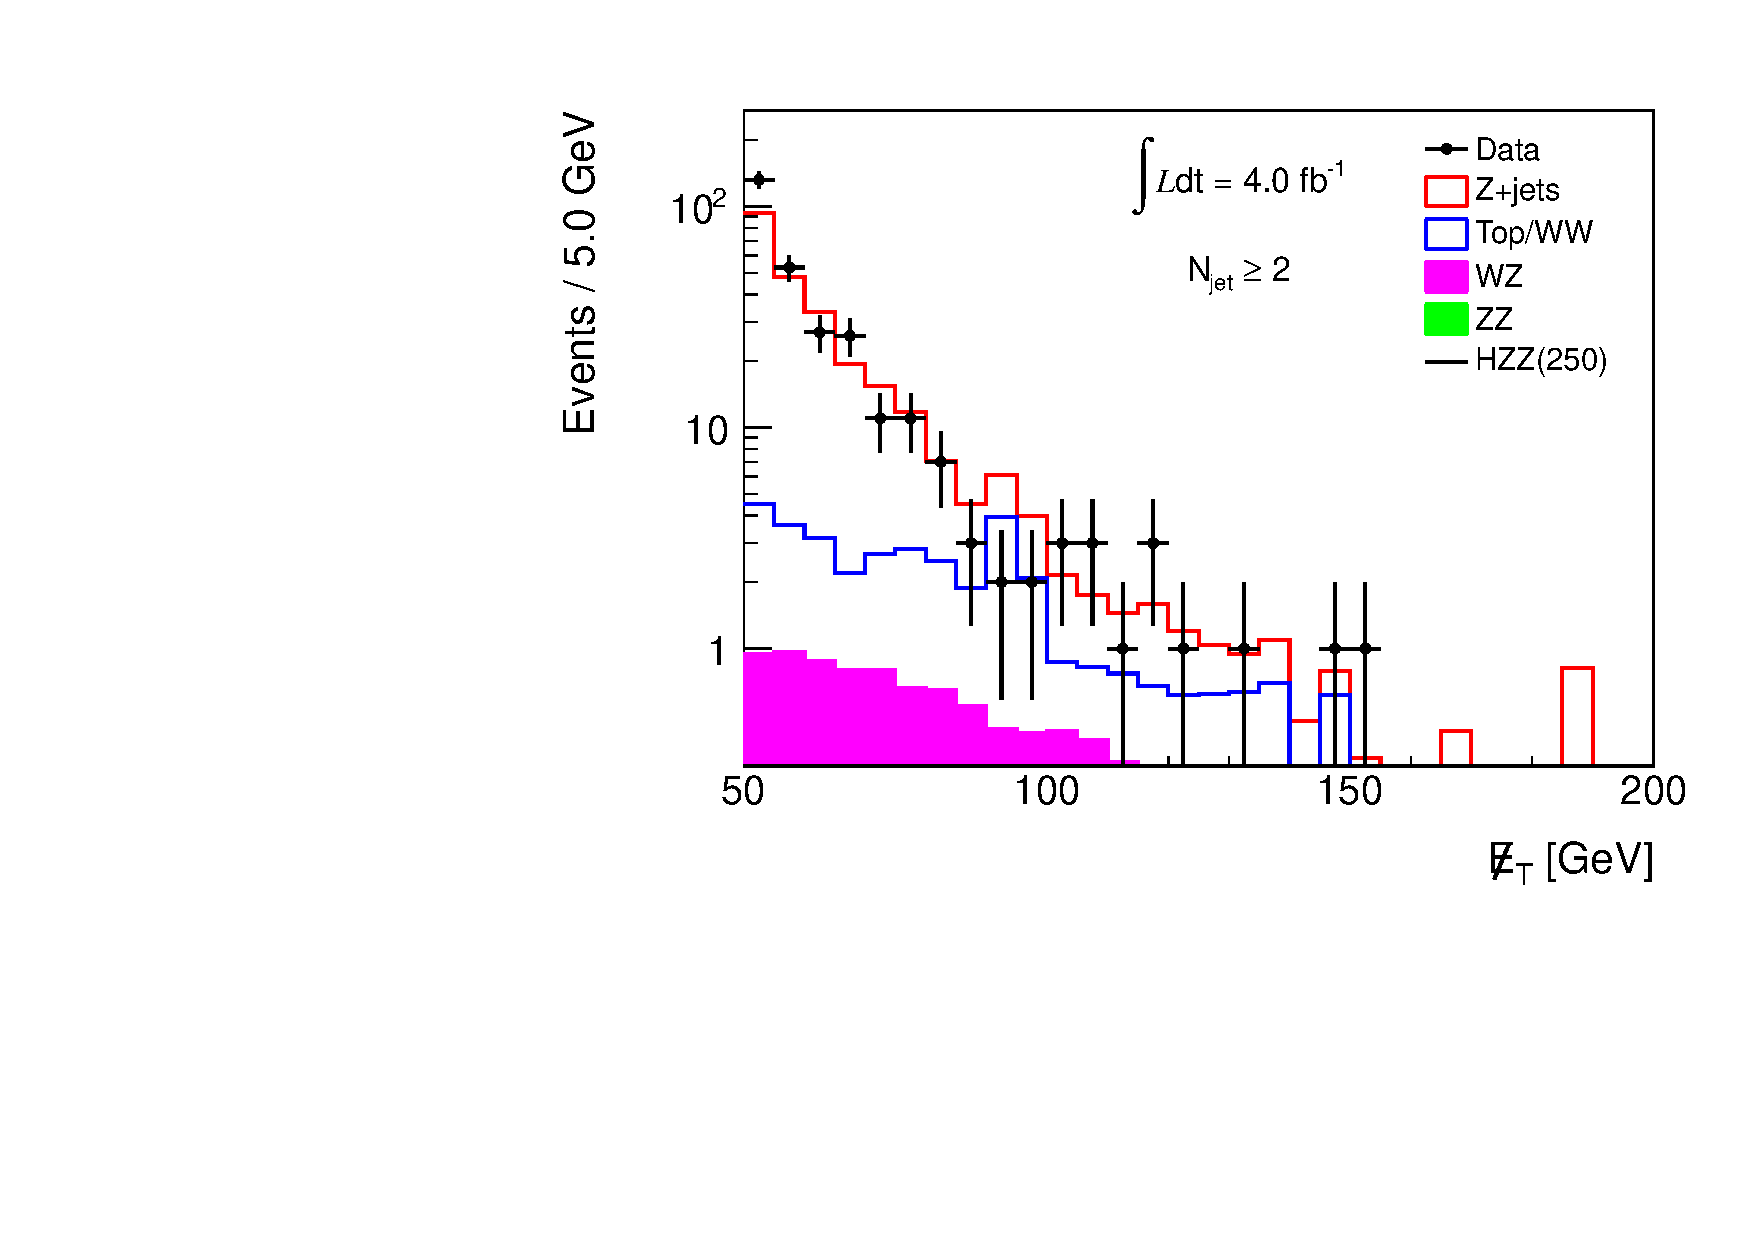
\includegraphics[width=.4\textwidth]{figures/presel_mH250_ee_metlog_2j.pdf}}
\caption{Missing transverse energy distribution in the electron channel after the $\ZZ$ preselection observed in data corresponding to $4.6$~\ifb data in 
the Inclusive~\subref{subfig:met_ee_incl}, 0-Jet~\subref{subfig:met_ee_0j}, 1-Jet~\subref{subfig:met_ee_1j} and $\geq$2-Jets~\subref{subfig:met_ee_2j} bins, 
compared to the expected from simulation for signal and background. The MC backgrounds are scaled as appropriate and the photon+jets estimate of the 
Z+jets background is added to the stack.}
\label{fig:met_zzpresel_ee}
\end{center}
\end{figure}
%%%%%%%%

%%%%%%%%
\begin{figure}[!hbtp]
\begin{center}
\subfigure[Inclusive]{\label{subfig:mt_mm_incl}
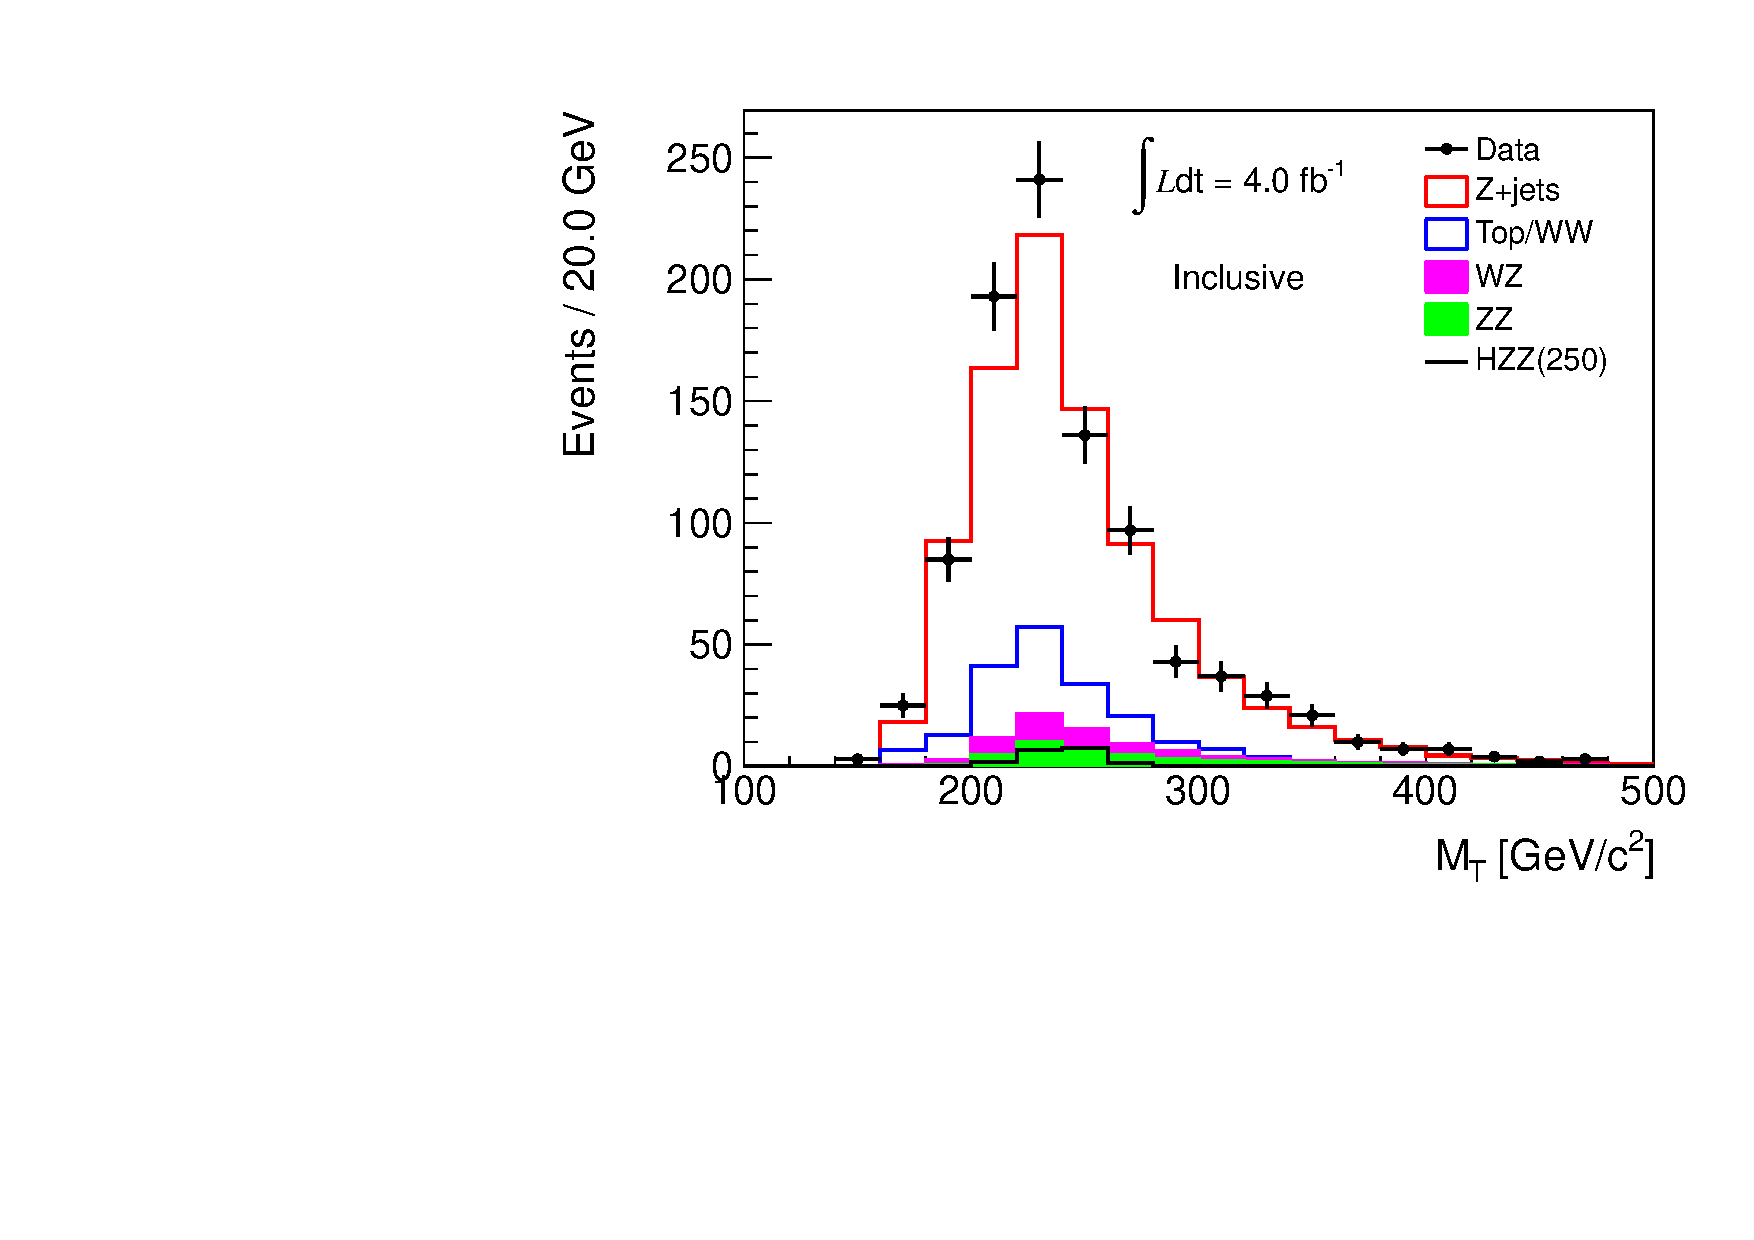
\includegraphics[width=.4\textwidth]{figures/presel_mH250_mm_mt_incl.pdf}}
\subfigure[0-Jet]{\label{subfig:mt_mm_0j}
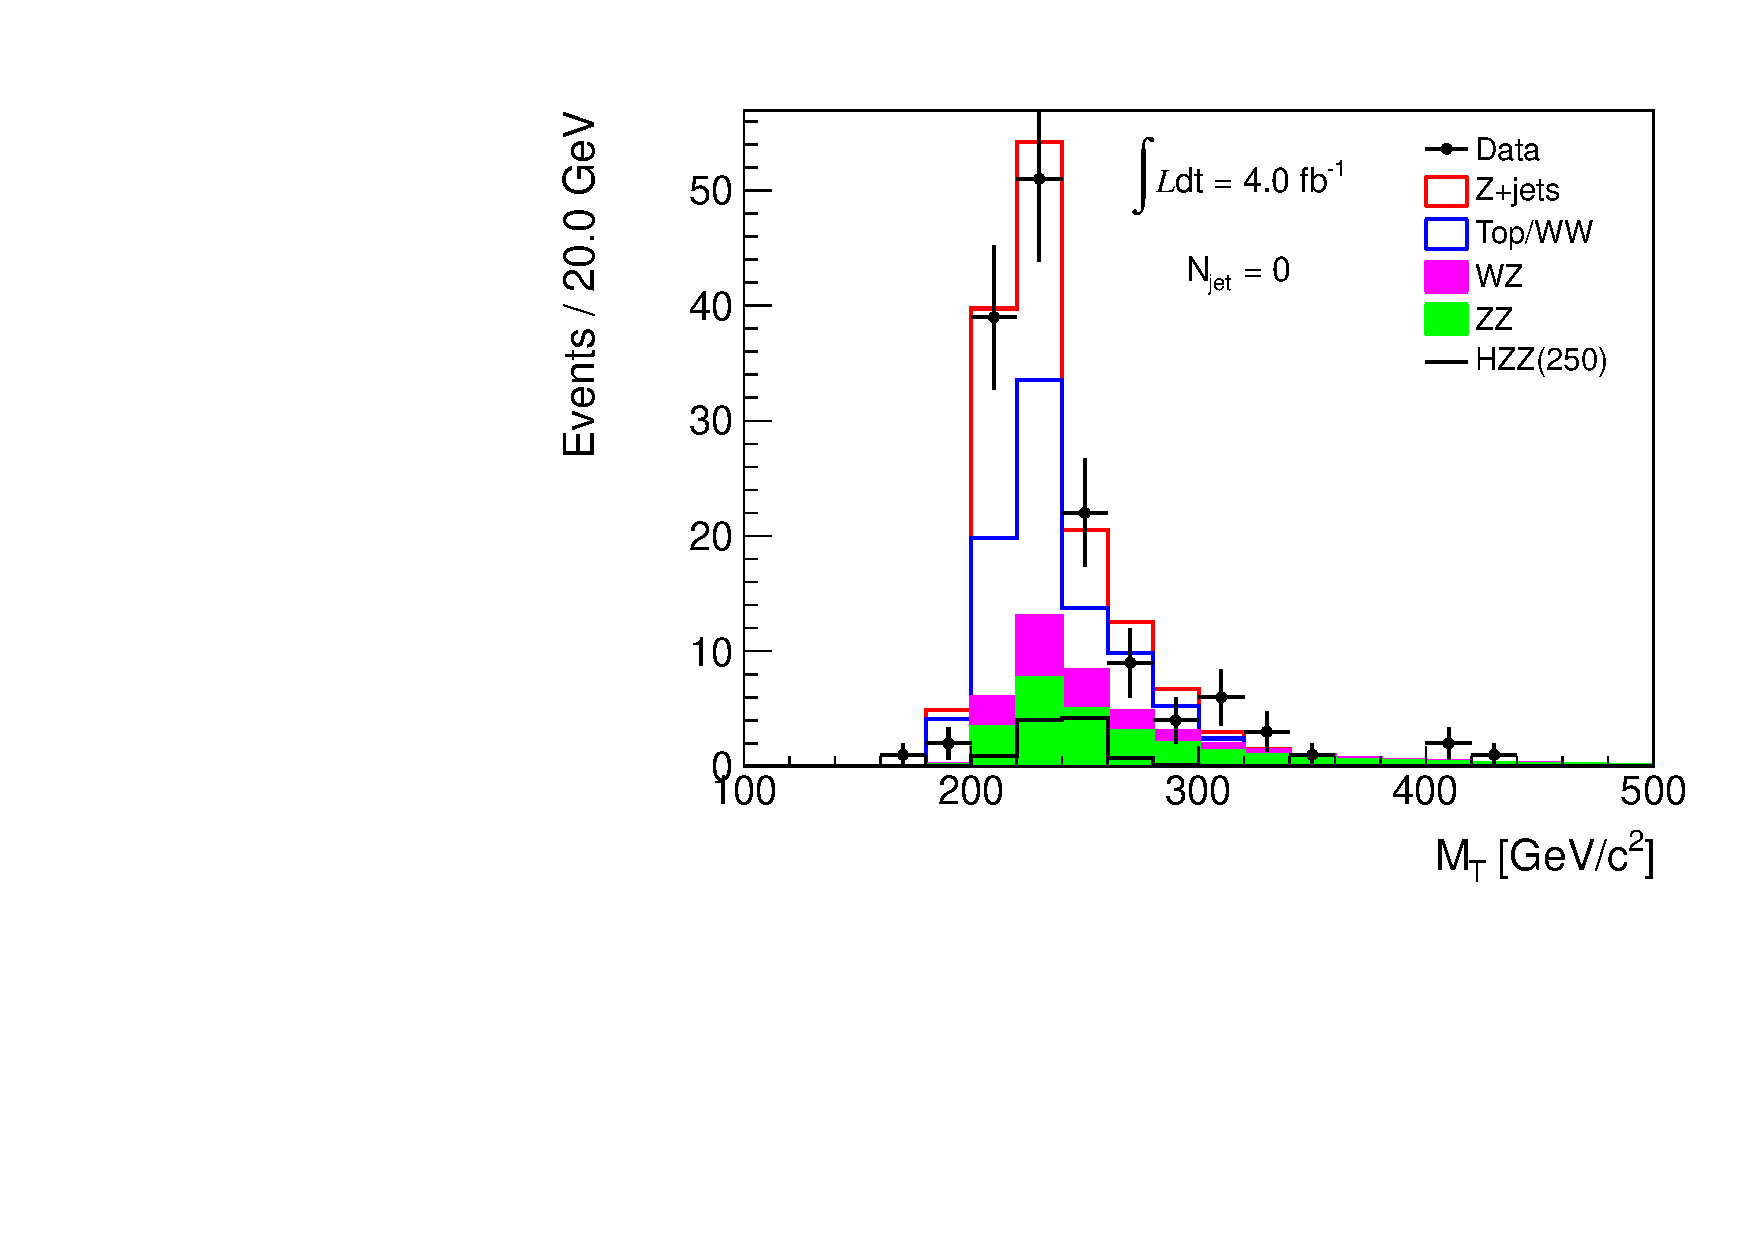
\includegraphics[width=.4\textwidth]{figures/presel_mH250_mm_mt_0j.pdf}} \\
\subfigure[1-Jet]{\label{subfig:mt_mm_1j}
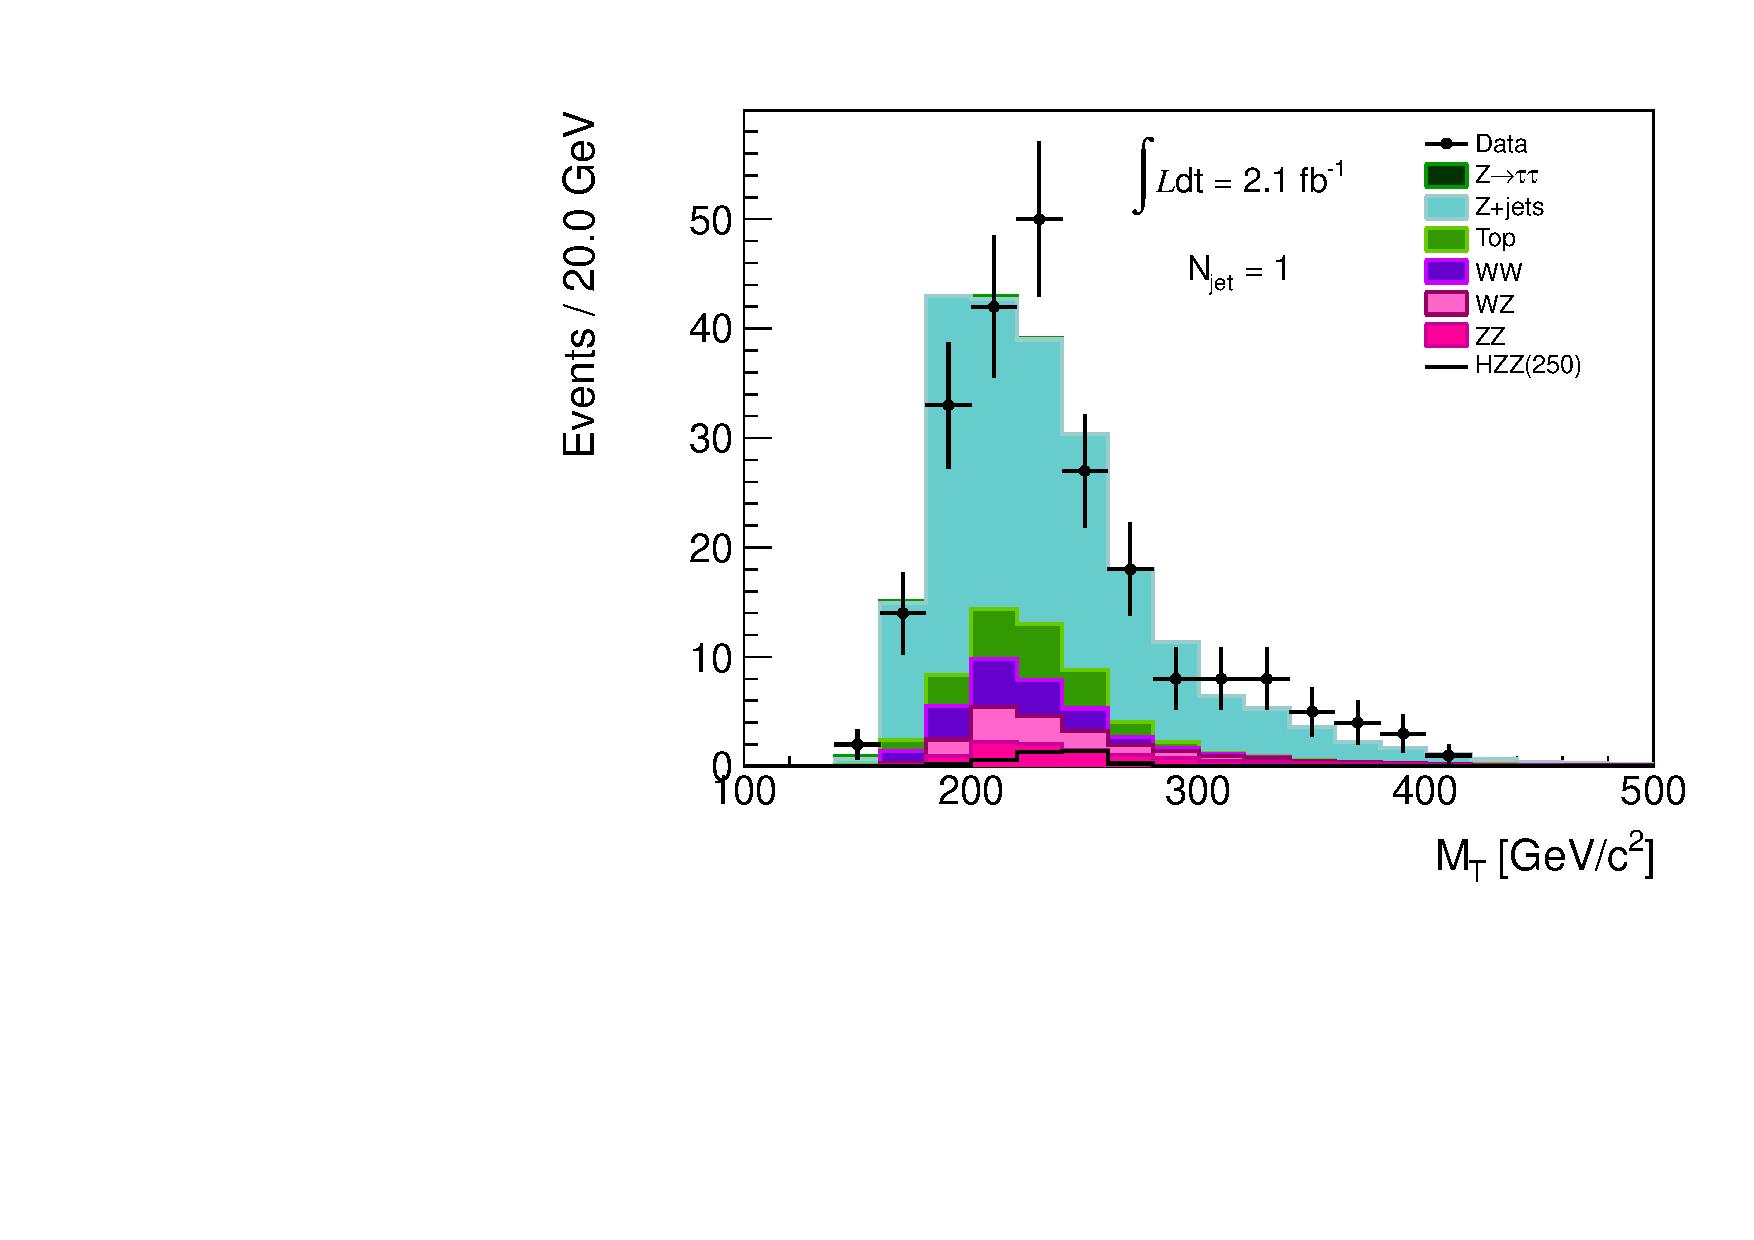
\includegraphics[width=.4\textwidth]{figures/presel_mH250_mm_mt_1j.pdf}}
\subfigure[$\geq$2 Jets]{\label{subfig:mt_mm_2j}
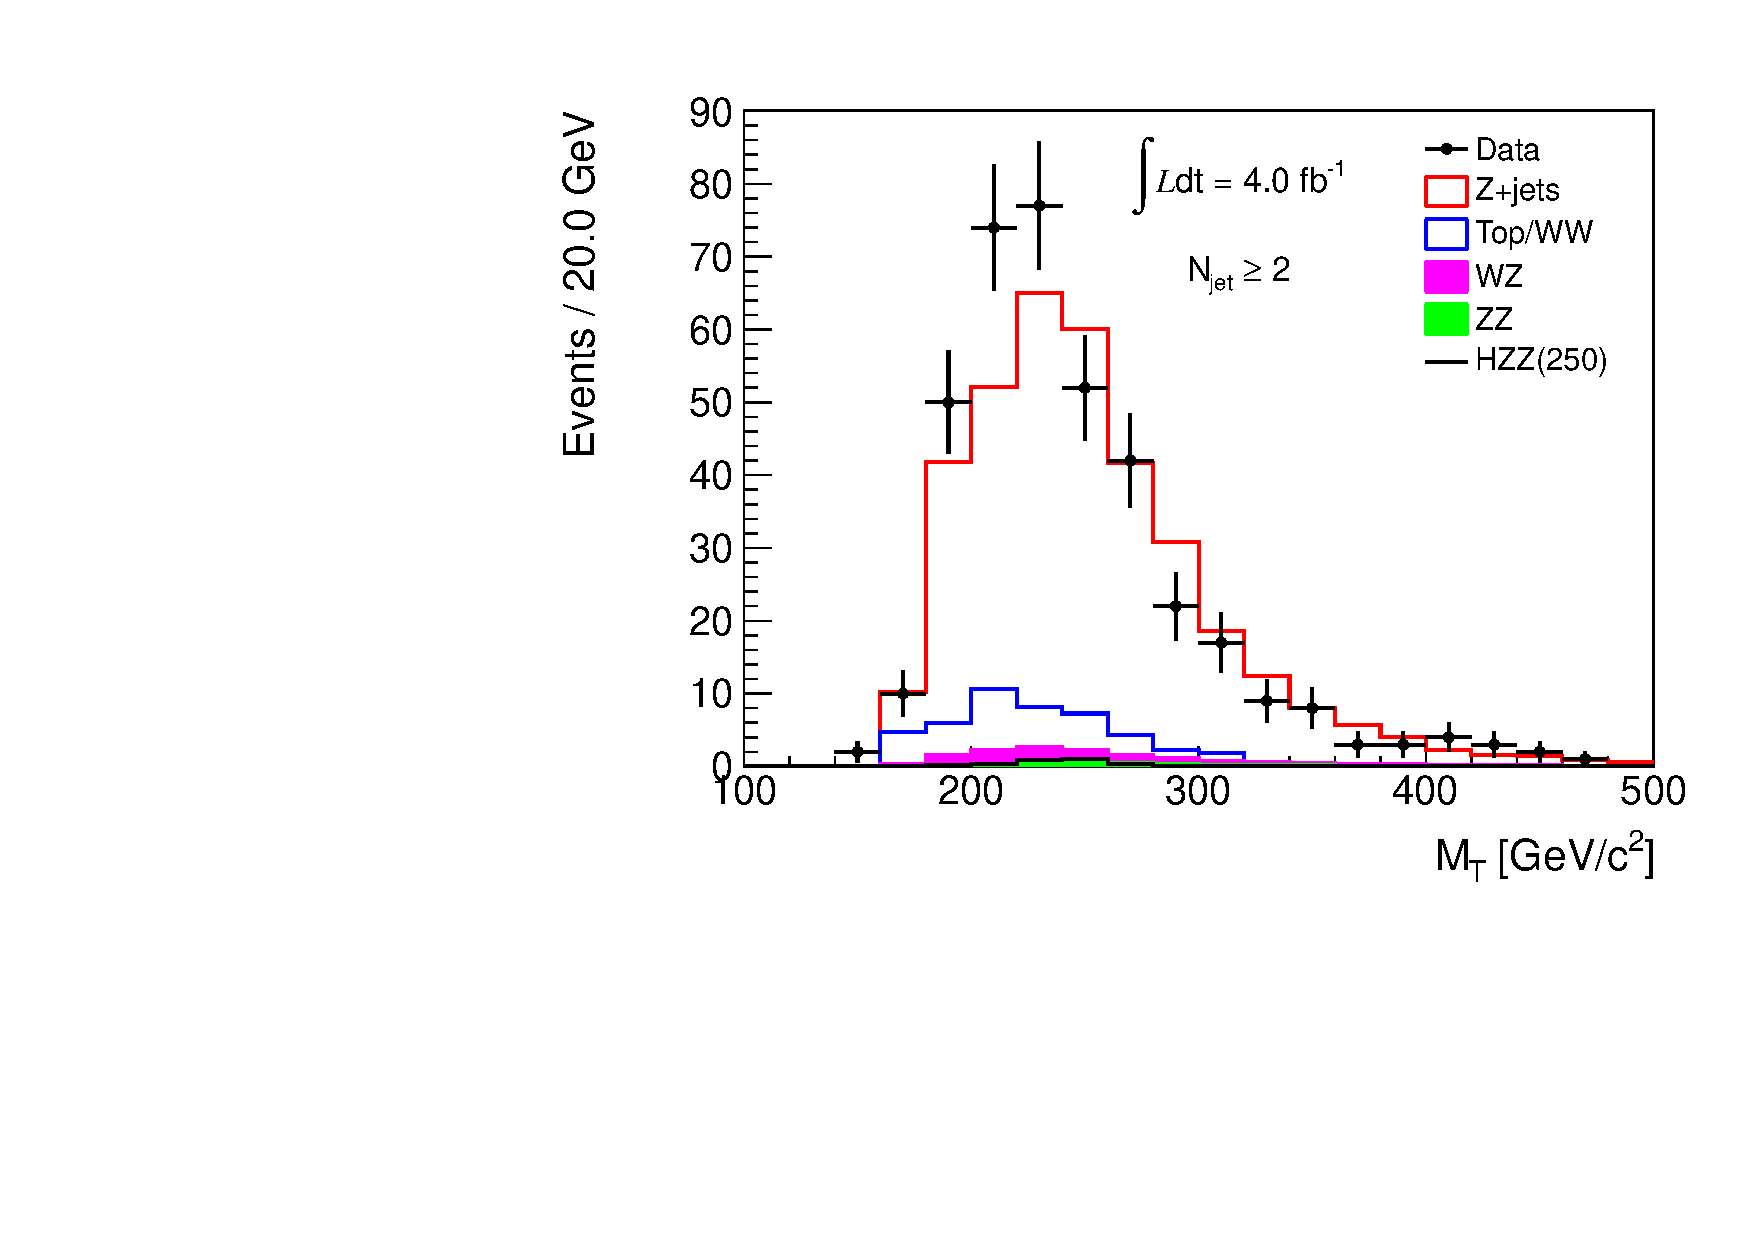
\includegraphics[width=.4\textwidth]{figures/presel_mH250_mm_mt_2j.pdf}}
\caption{Transverse mass distribution in the muon channel after the $\ZZ$ preselection observed in data corresponding to $4.6$~\ifb data in 
the Inclusive~\subref{subfig:mt_mm_incl}, 0-Jet~\subref{subfig:mt_mm_0j}, 1-Jet~\subref{subfig:mt_mm_1j} and $\geq$2-Jets~\subref{subfig:mt_mm_2j} bins, 
compared to the expected from simulation for signal and background. The MC backgrounds are scaled as appropriate and the photon+jets estimate of the 
Z+jets background is added to the stack.}
\label{fig:mt_zzpresel_mm}
\end{center}
\end{figure}
%%%%%%%%

%%%%%%%%
\begin{figure}[!hbtp]
\begin{center}
\subfigure[Inclusive]{\label{subfig:mt_ee_incl}
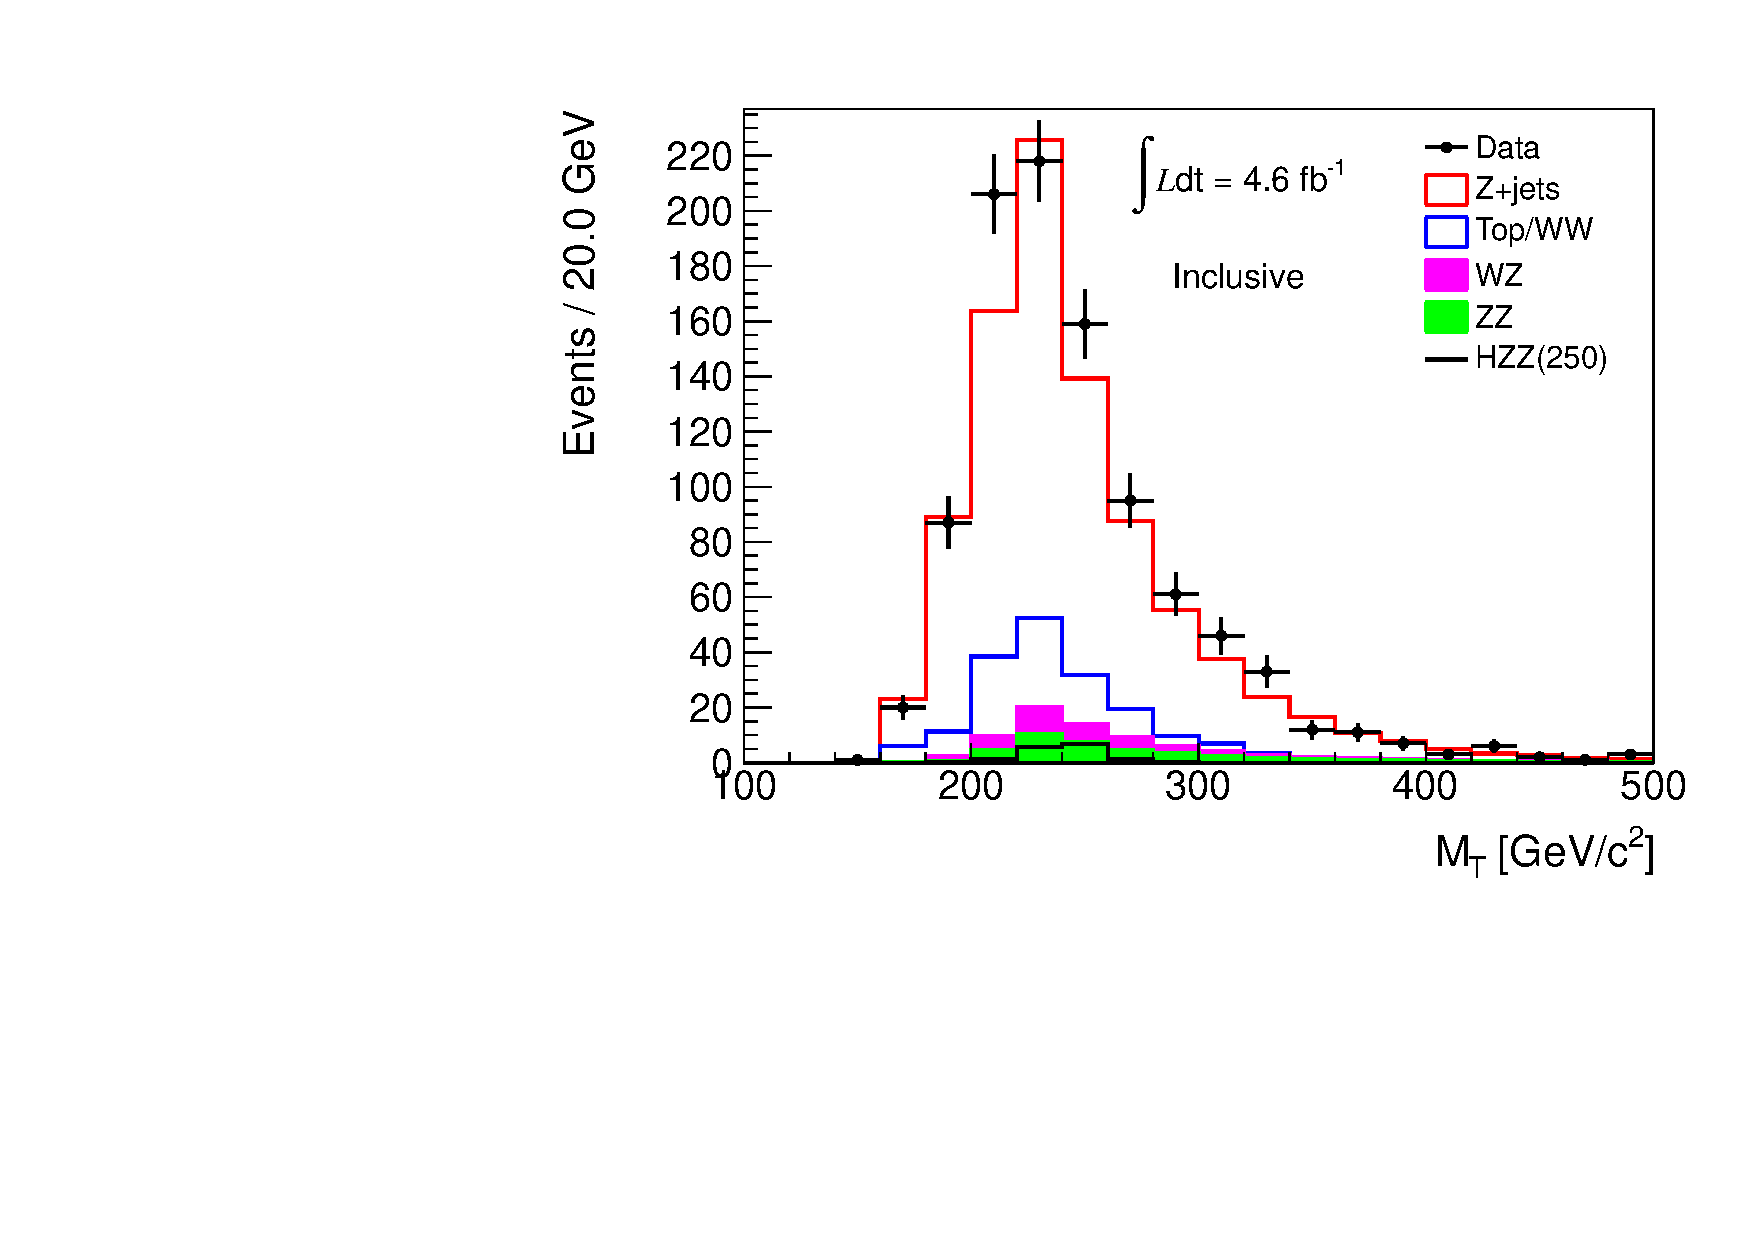
\includegraphics[width=.4\textwidth]{figures/presel_mH250_ee_mt_incl.pdf}}
\subfigure[0-Jet]{\label{subfig:mt_ee_0j}
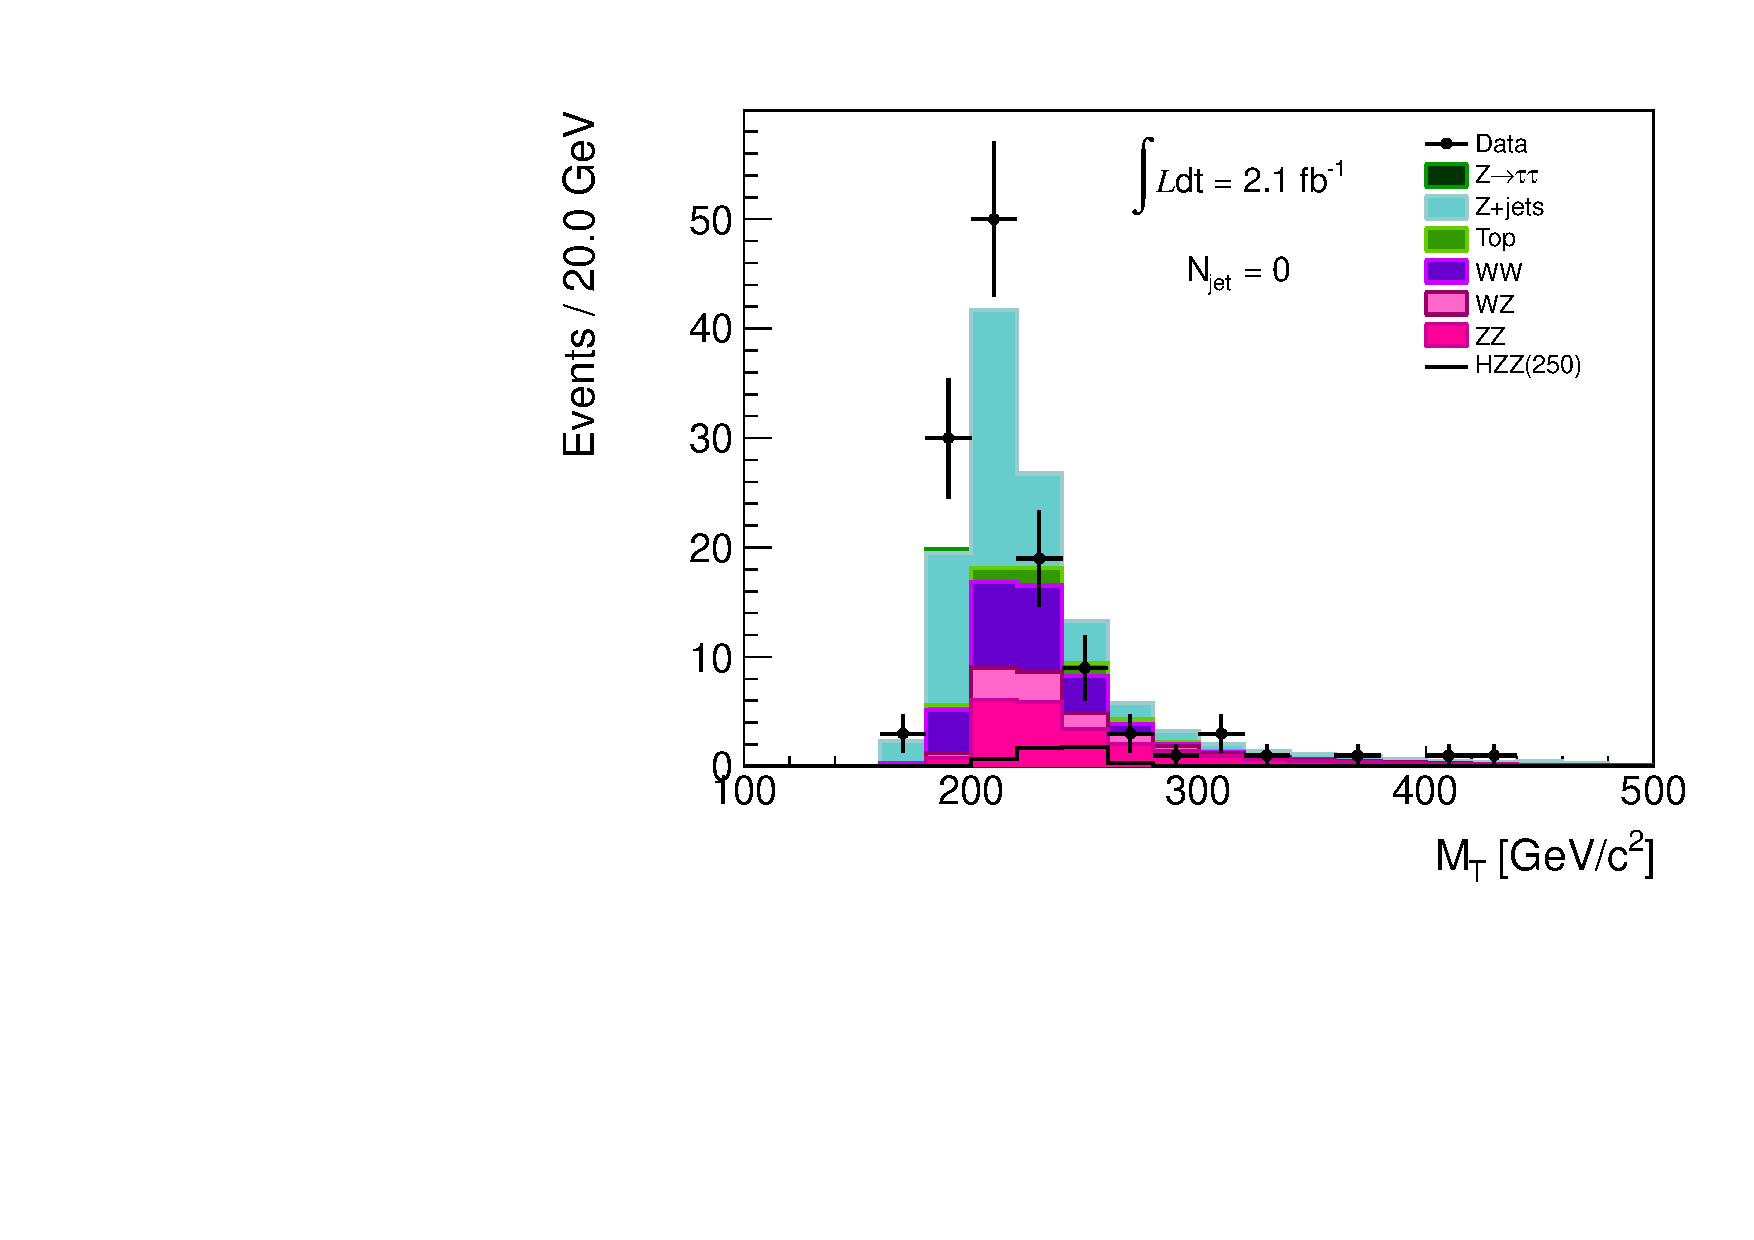
\includegraphics[width=.4\textwidth]{figures/presel_mH250_ee_mt_0j.pdf}} \\
\subfigure[1-Jet]{\label{subfig:mt_ee_1j}
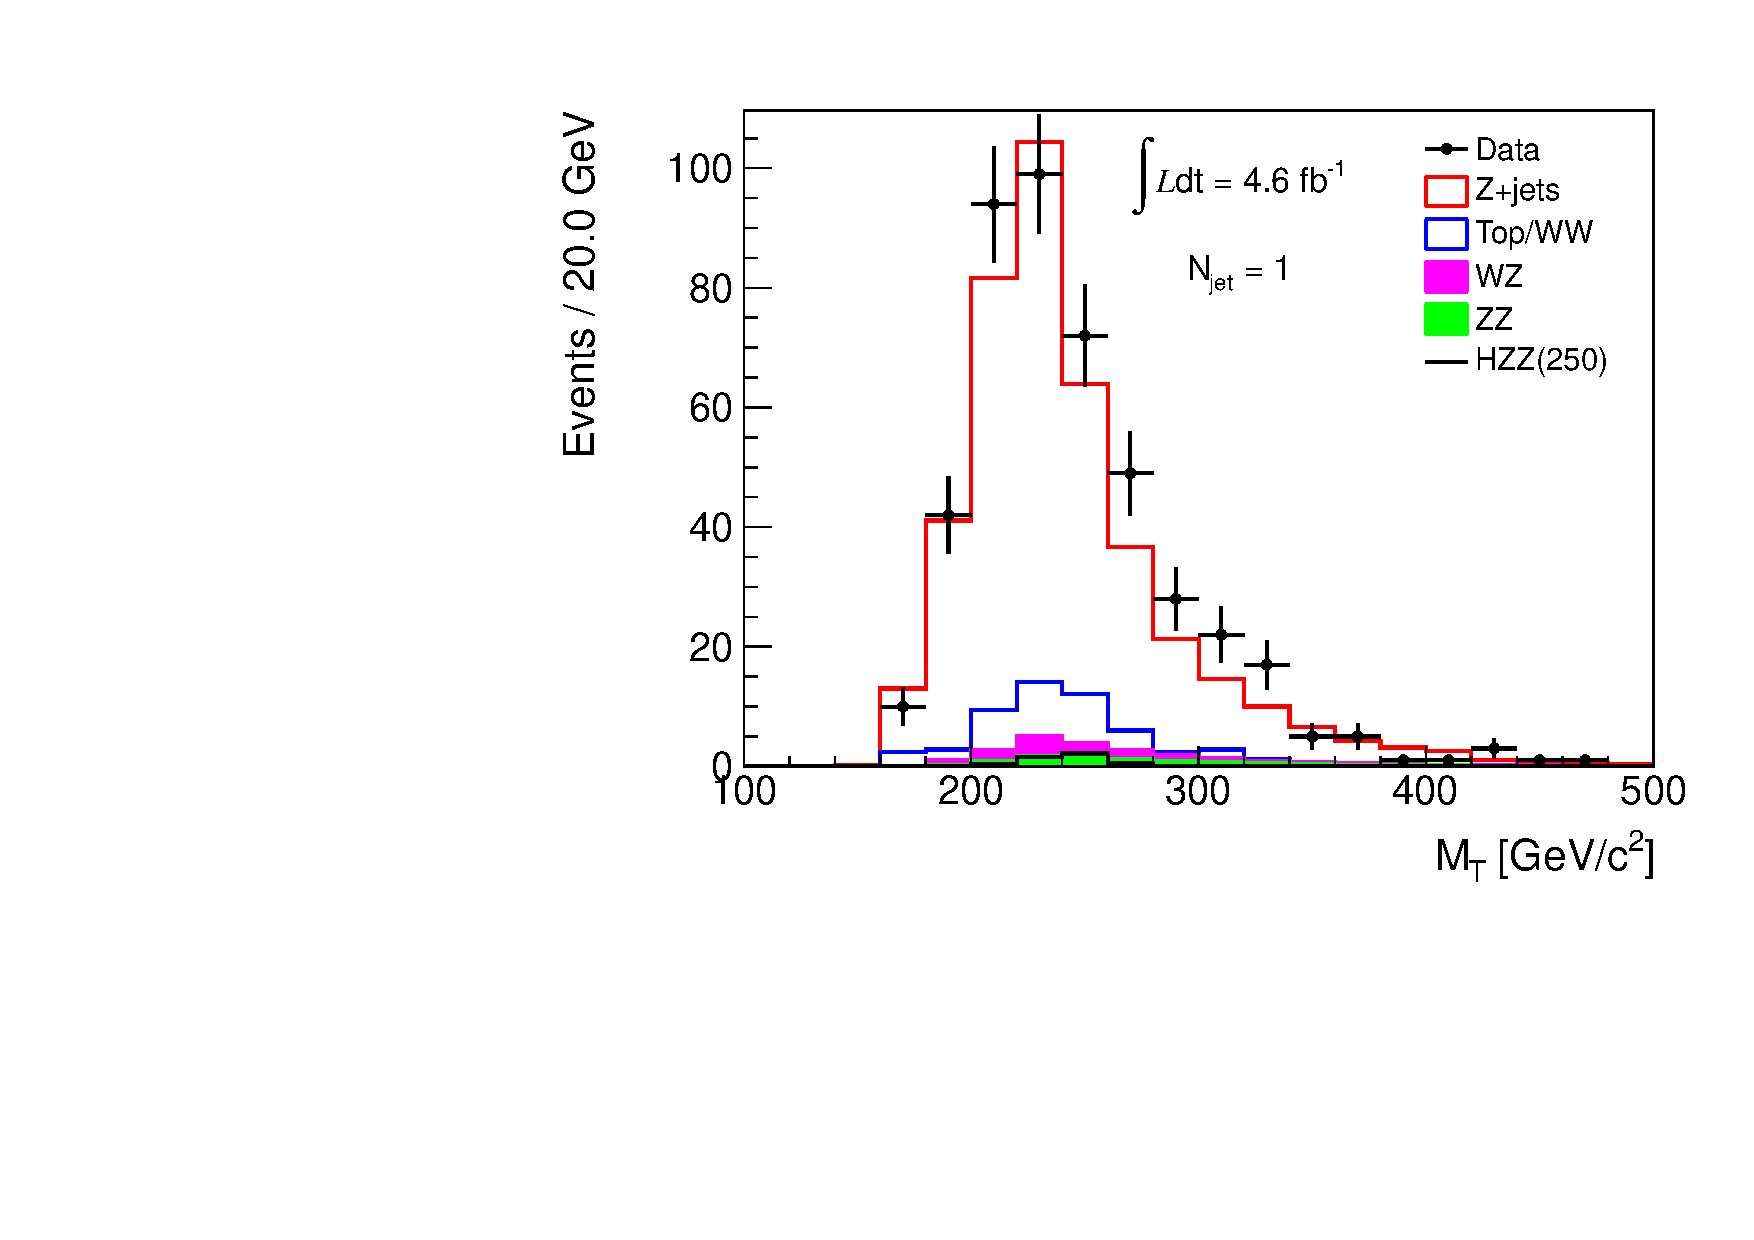
\includegraphics[width=.4\textwidth]{figures/presel_mH250_ee_mt_1j.pdf}}
\subfigure[$\geq$2 Jets]{\label{subfig:mt_ee_2j}
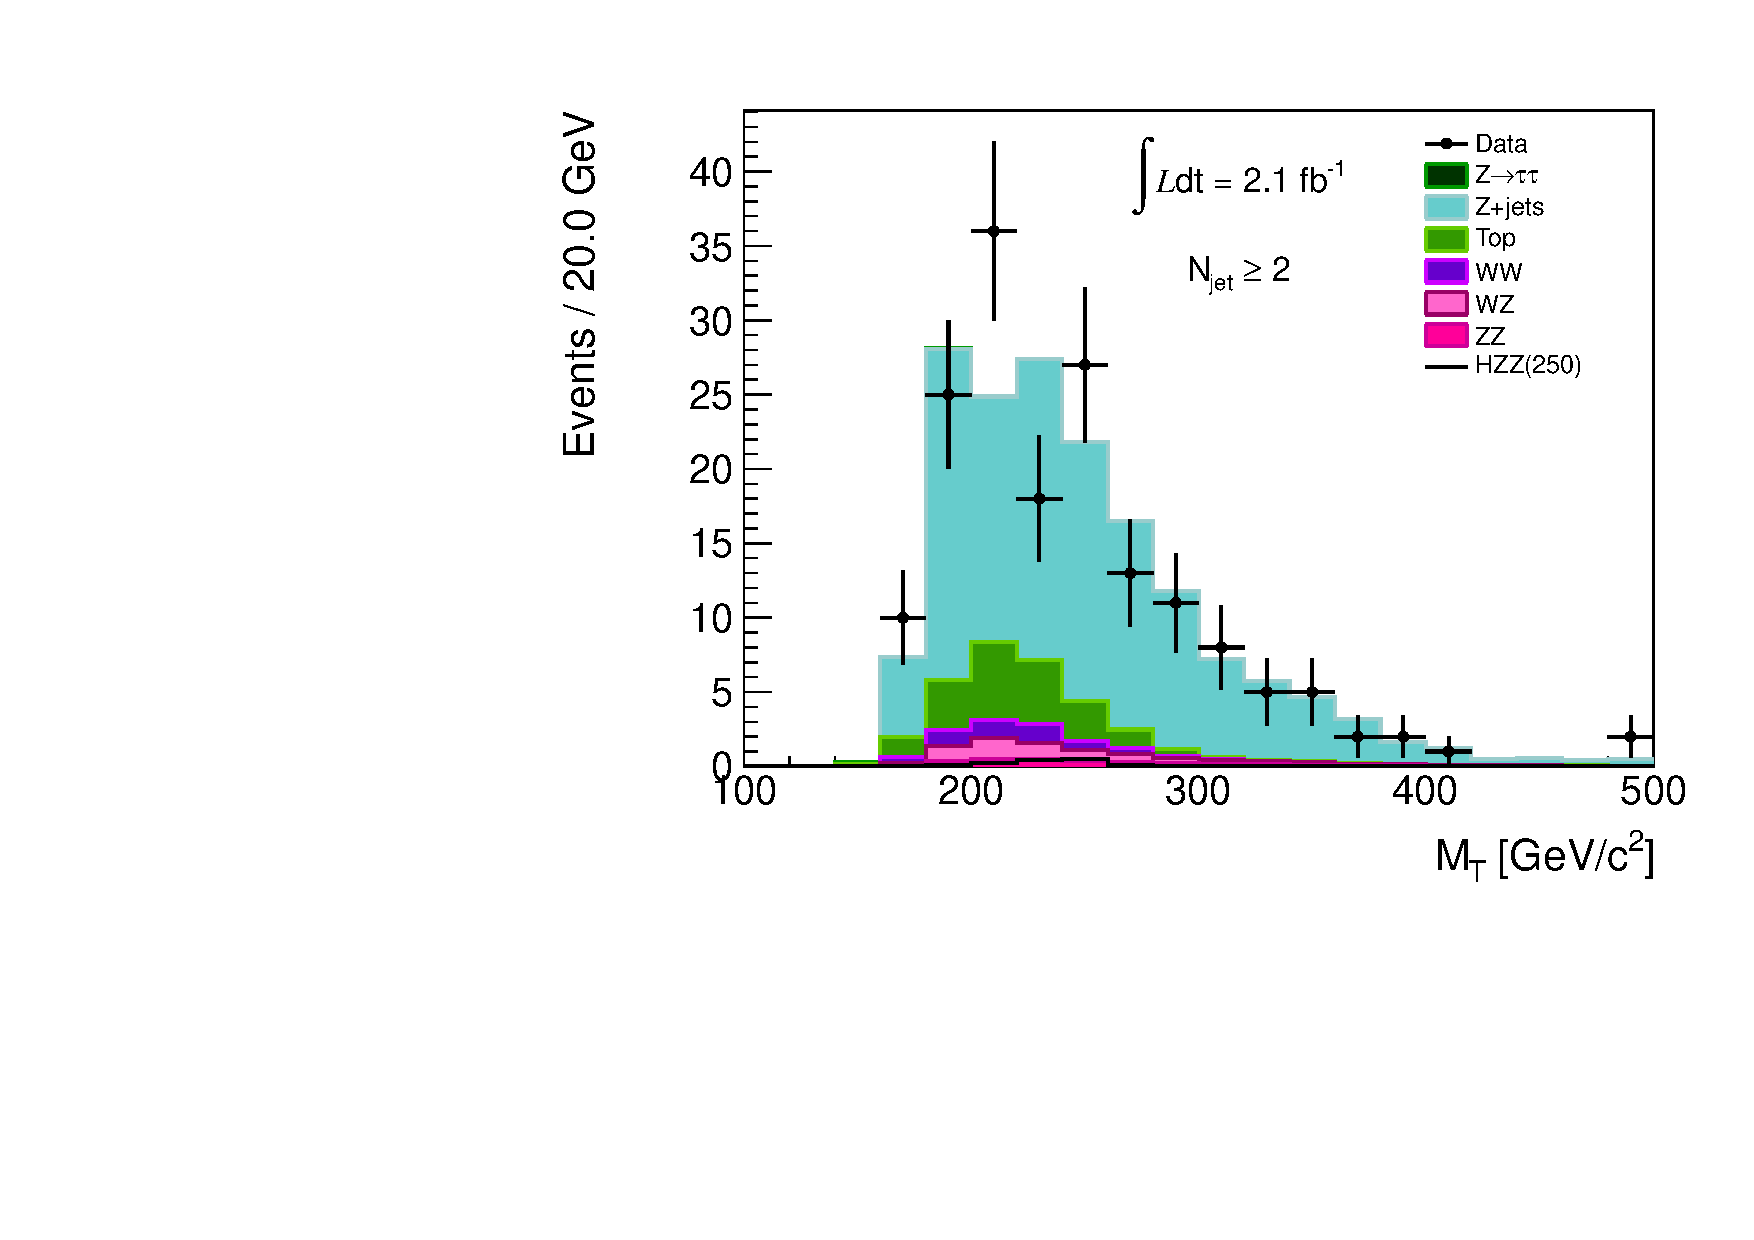
\includegraphics[width=.4\textwidth]{figures/presel_mH250_ee_mt_2j.pdf}}
\caption{Transverse mass distribution in the electron channel after the $\ZZ$ preselection observed in data corresponding to $4.6$~\ifb data in 
the Inclusive~\subref{subfig:mt_ee_incl}, 0-Jet~\subref{subfig:mt_ee_0j}, 1-Jet~\subref{subfig:mt_ee_1j} and $\geq$2-Jets~\subref{subfig:mt_ee_2j} bins, 
compared to the expected from simulation for signal and background. The MC backgrounds are scaled as appropriate and the photon+jets estimate of the 
Z+jets background is added to the stack.}
\label{fig:mt_zzpresel_ee}
\end{center}
\end{figure}
%%%%%%%%

%%%%%%%%
\begin{figure}[!hbtp]
\begin{center}
\subfigure[$\geq$1 Jets]{\label{subfig:dphijetmet_mm_incl}
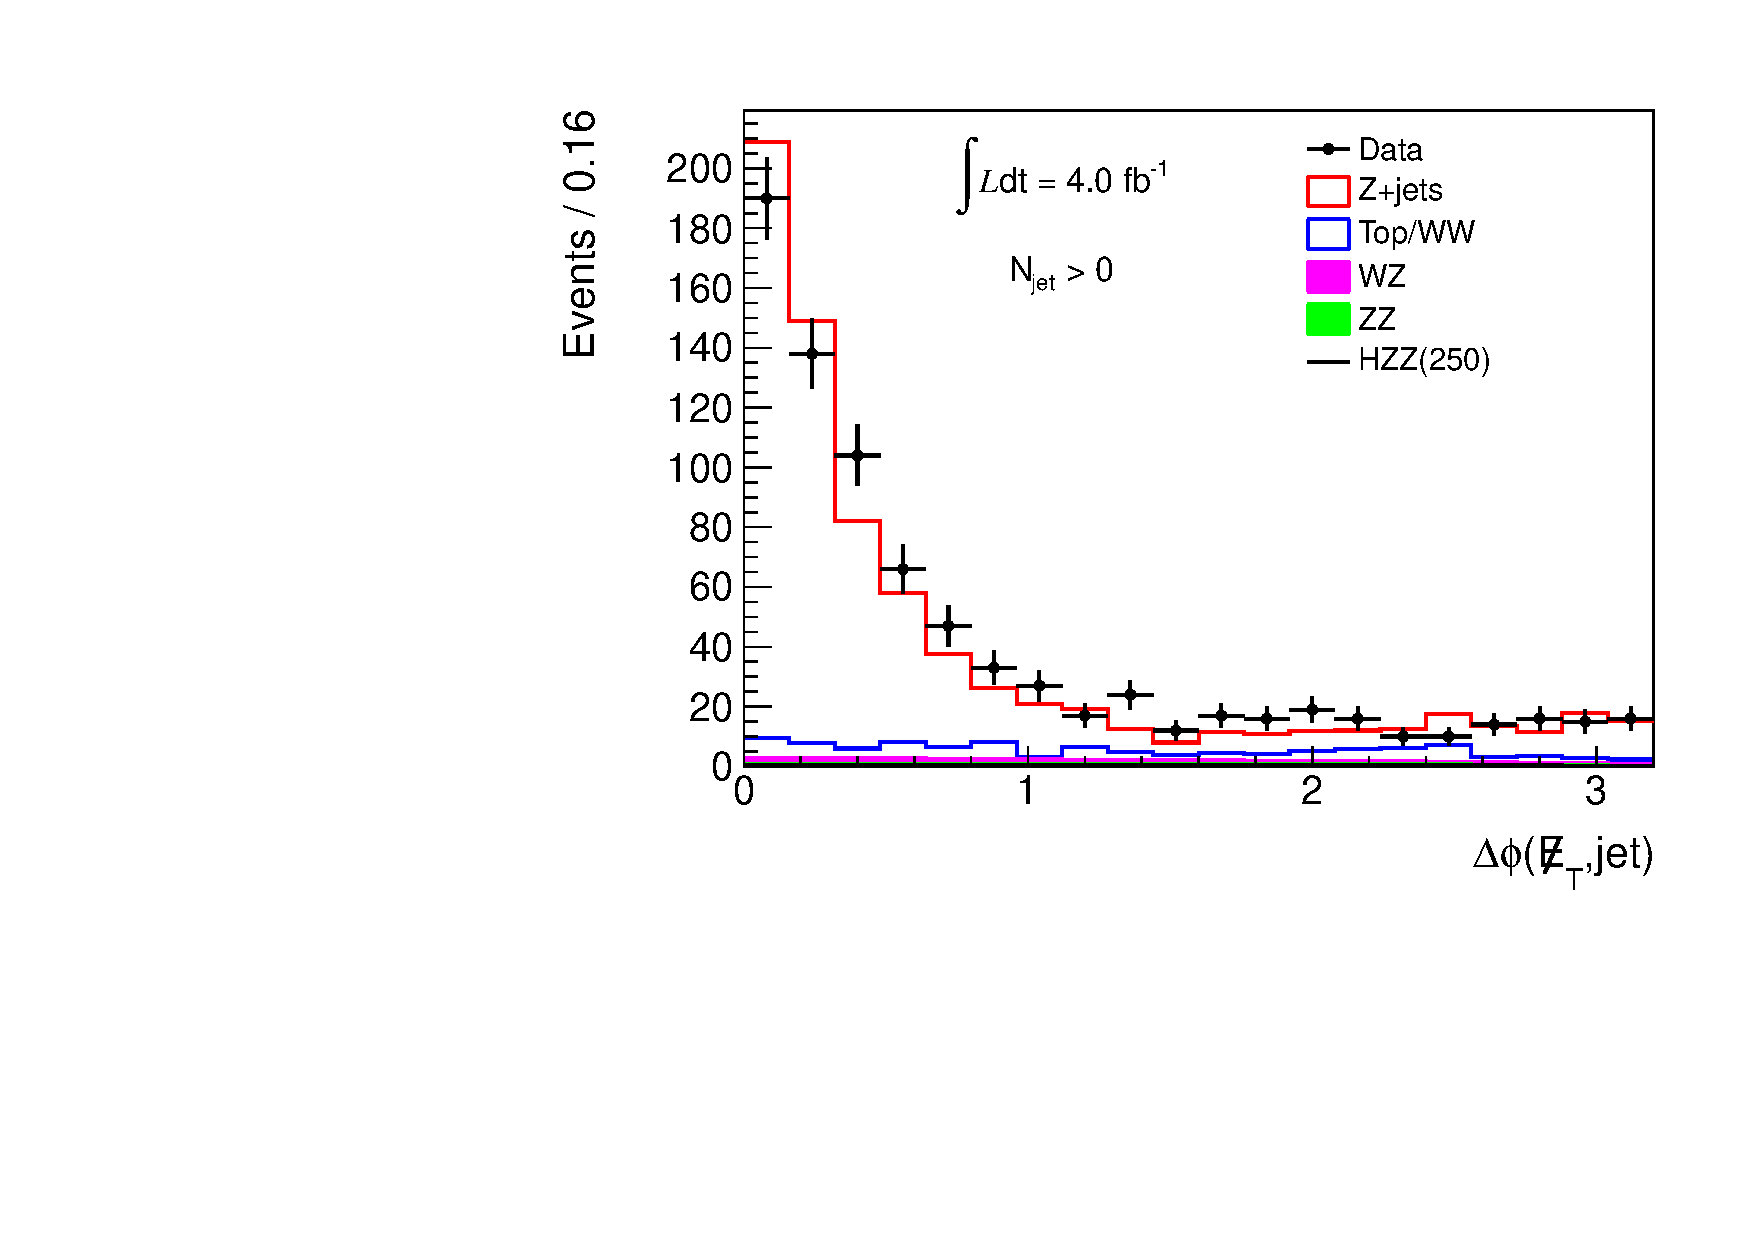
\includegraphics[width=.3\textwidth]{figures/presel_mH250_mm_dphijetmet_incl.pdf}}
\subfigure[1-Jet]{\label{subfig:dphijetmet_mm_1j}
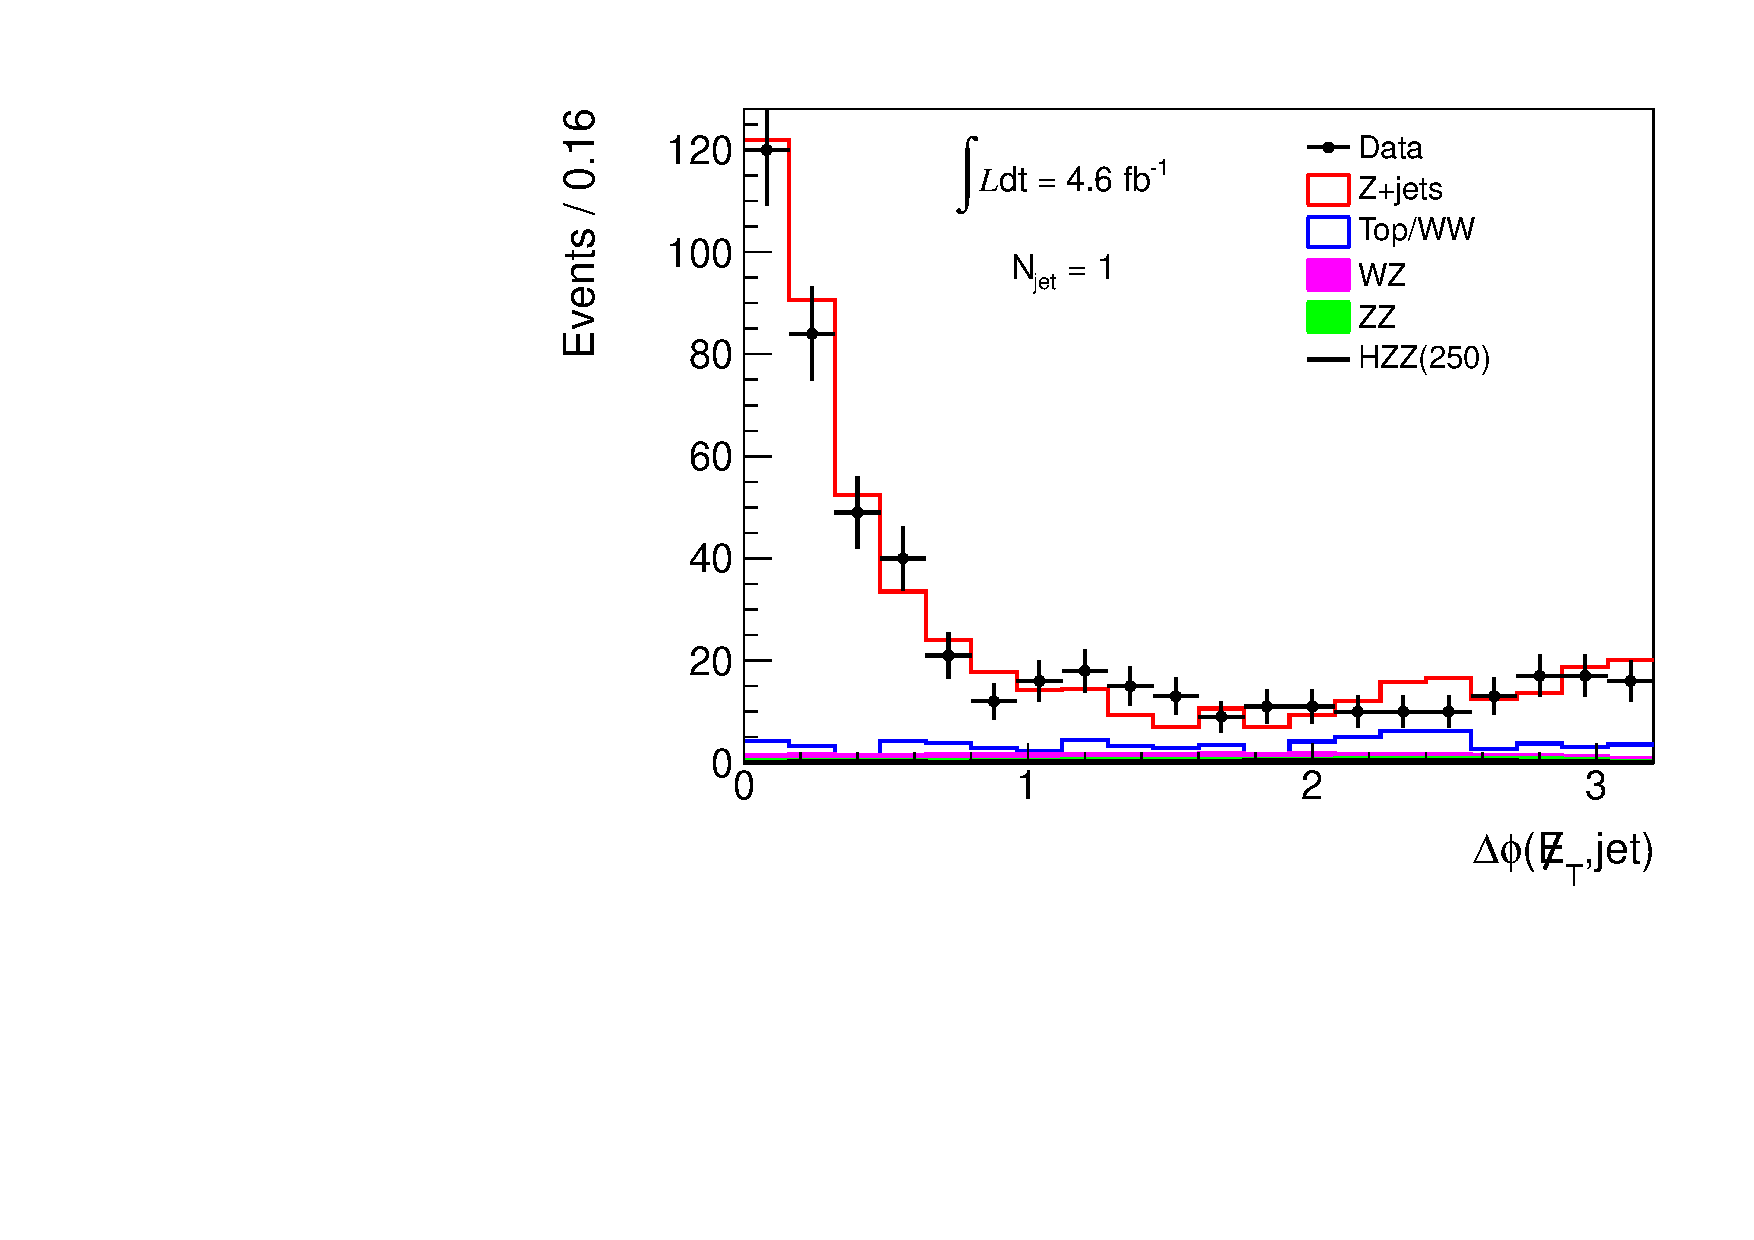
\includegraphics[width=.3\textwidth]{figures/presel_mH250_mm_dphijetmet_1j.pdf}}
\subfigure[$\geq$2 Jets]{\label{subfig:dphijetmet_mm_2j}
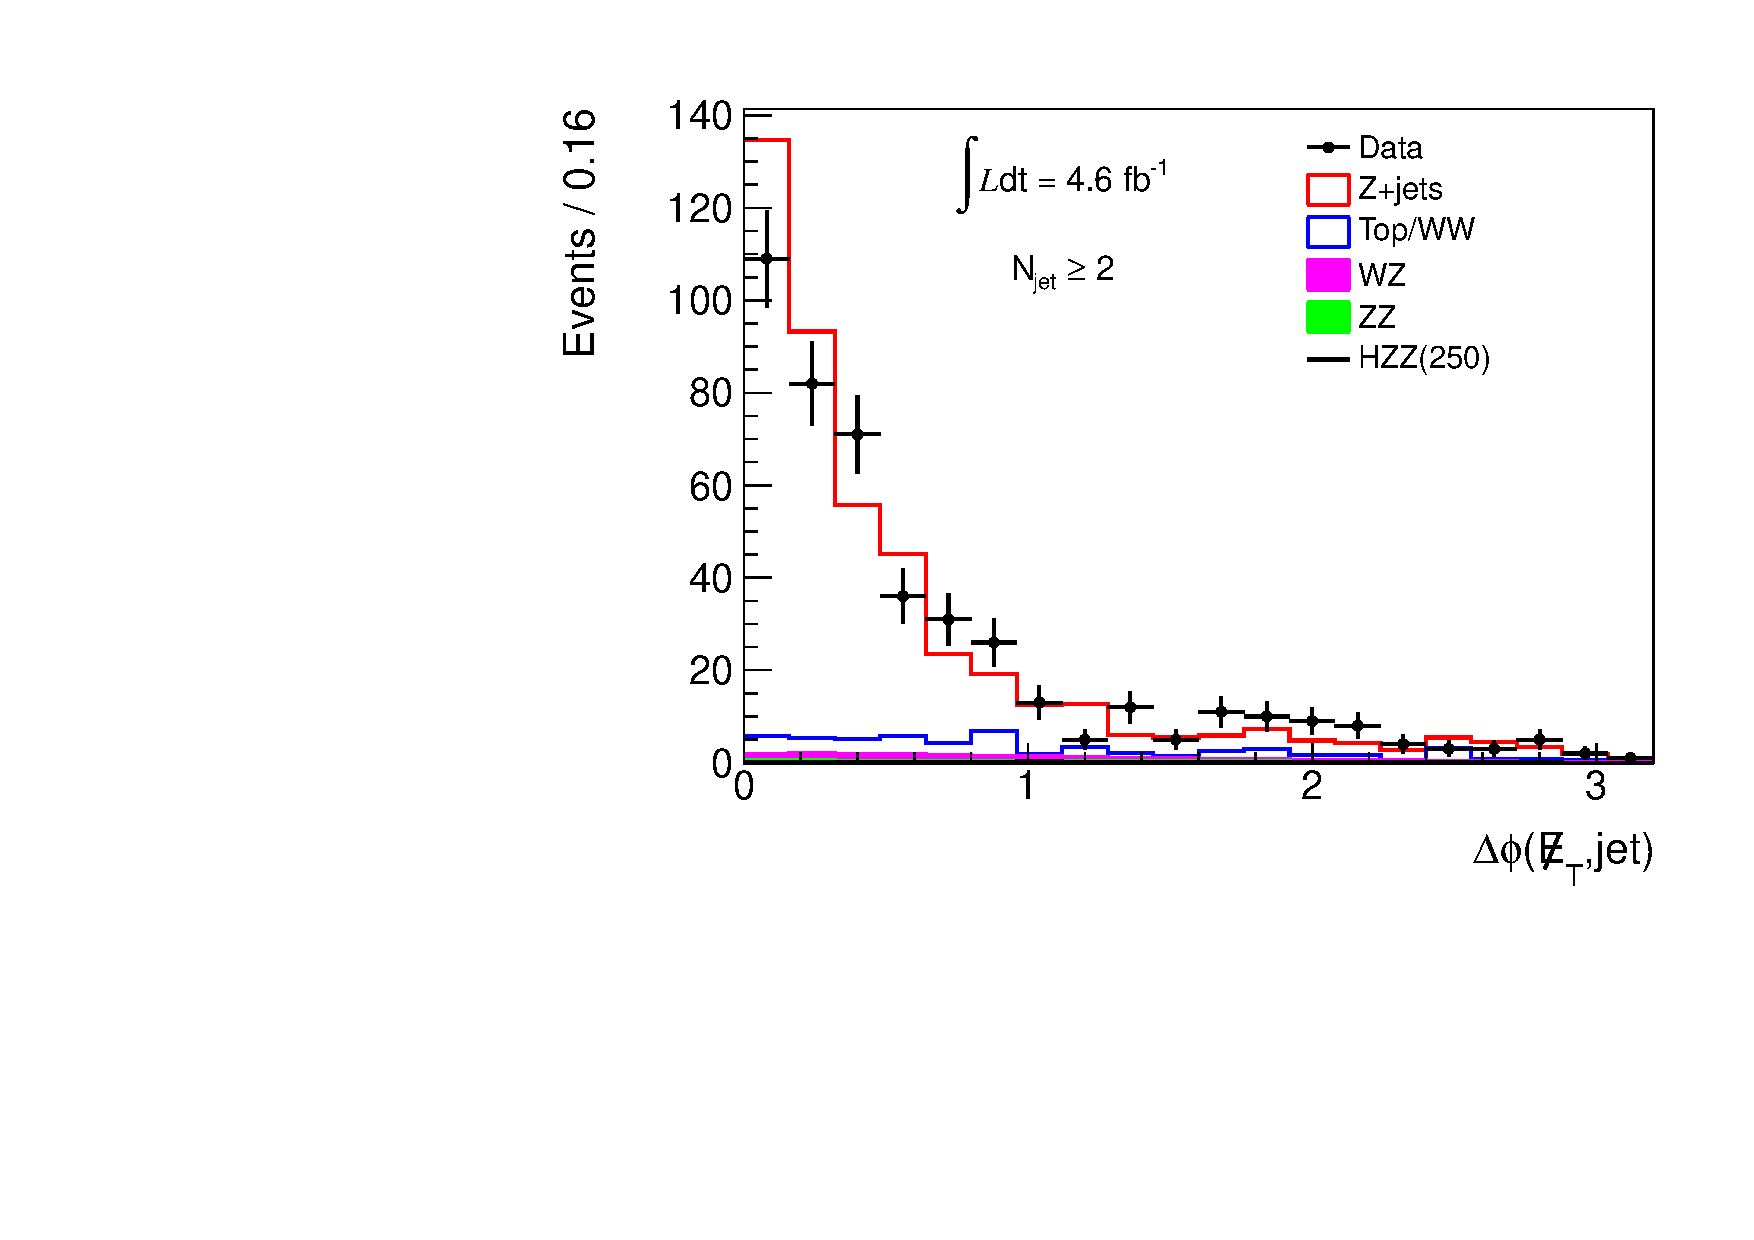
\includegraphics[width=.3\textwidth]{figures/presel_mH250_mm_dphijetmet_2j.pdf}}
\caption{Azimuthal angle separation between \met and the closest jet in the muon channel after the $\ZZ$ preselection observed in data corresponding 
to $4.6$~\ifb data in the $\geq$1 Jets~\subref{subfig:dphijetmet_mm_incl}, 1-Jet~\subref{subfig:dphijetmet_mm_1j} and 
$\geq$2-Jets~\subref{subfig:dphijetmet_mm_2j} bins, compared to the expected from simulation for signal and background. The MC backgrounds are scaled as appropriate and 
the photon+jets estimate of the Z+jets background is added to the stack.}
\label{fig:dphijetmet_zzpresel_mm}
\end{center}
%\end{figure}

%\begin{figure}[!hbtp]
\begin{center}
\subfigure[$\geq$1 Jets]{\label{subfig:dphijetmet_ee_incl}
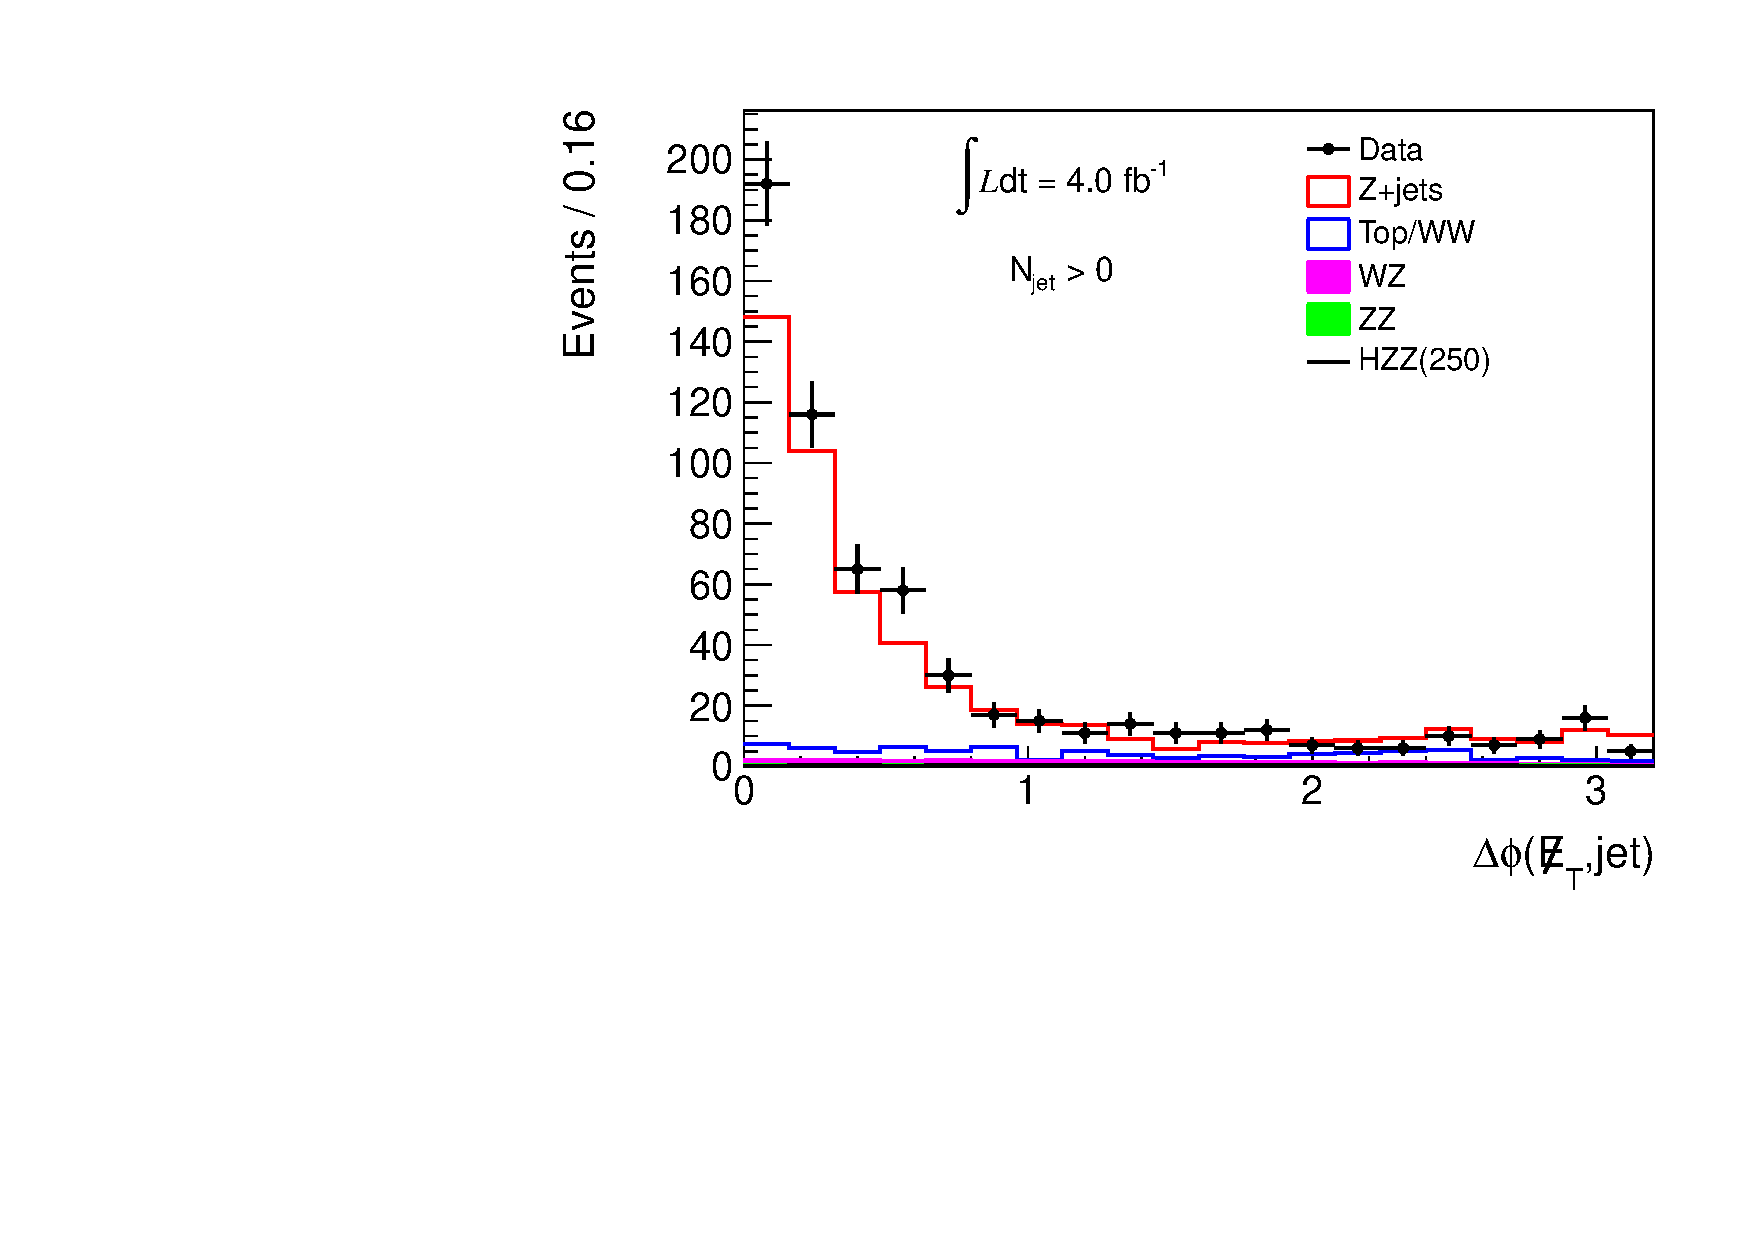
\includegraphics[width=.3\textwidth]{figures/presel_mH250_ee_dphijetmet_incl.pdf}}
\subfigure[1-Jet]{\label{subfig:dphijetmet_ee_1j}
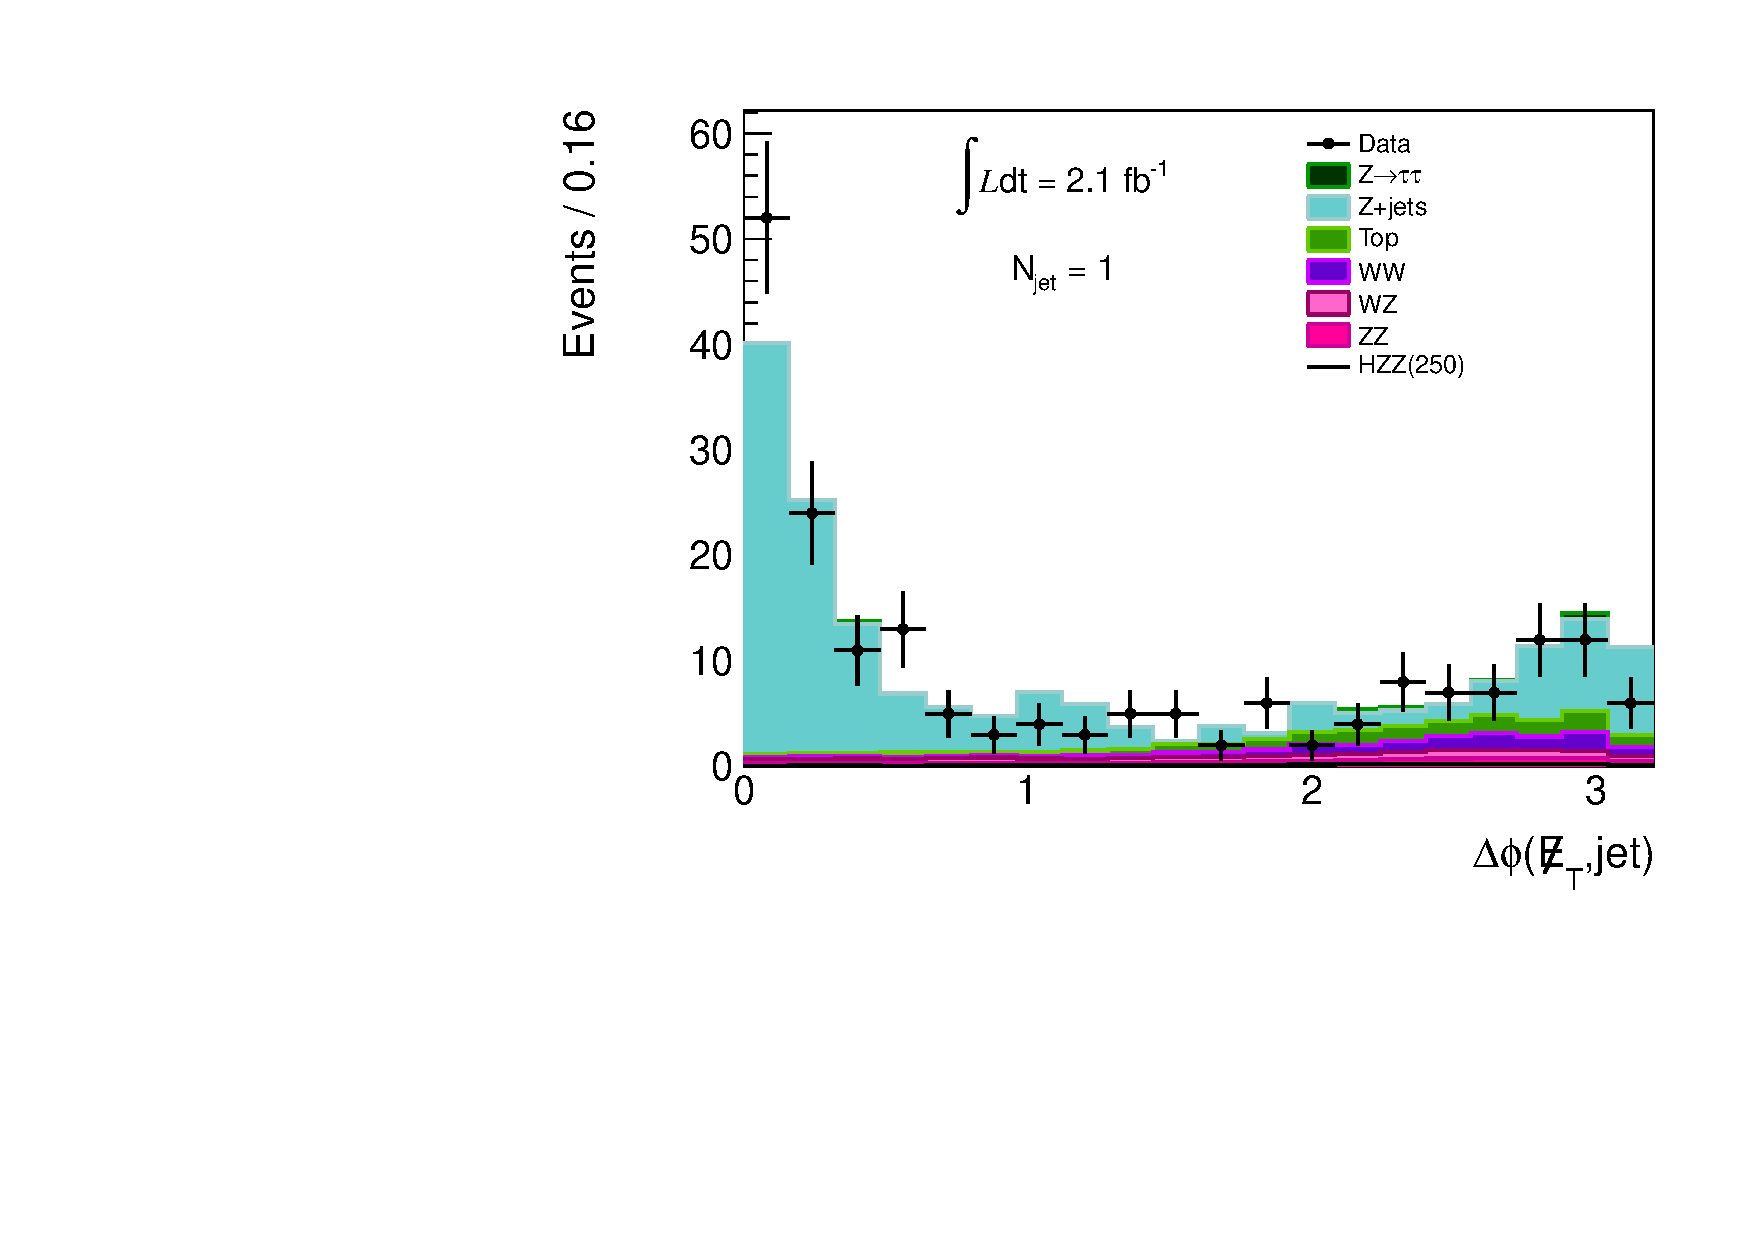
\includegraphics[width=.3\textwidth]{figures/presel_mH250_ee_dphijetmet_1j.pdf}}
\subfigure[$\geq$2 Jets]{\label{subfig:dphijetmet_ee_2j}
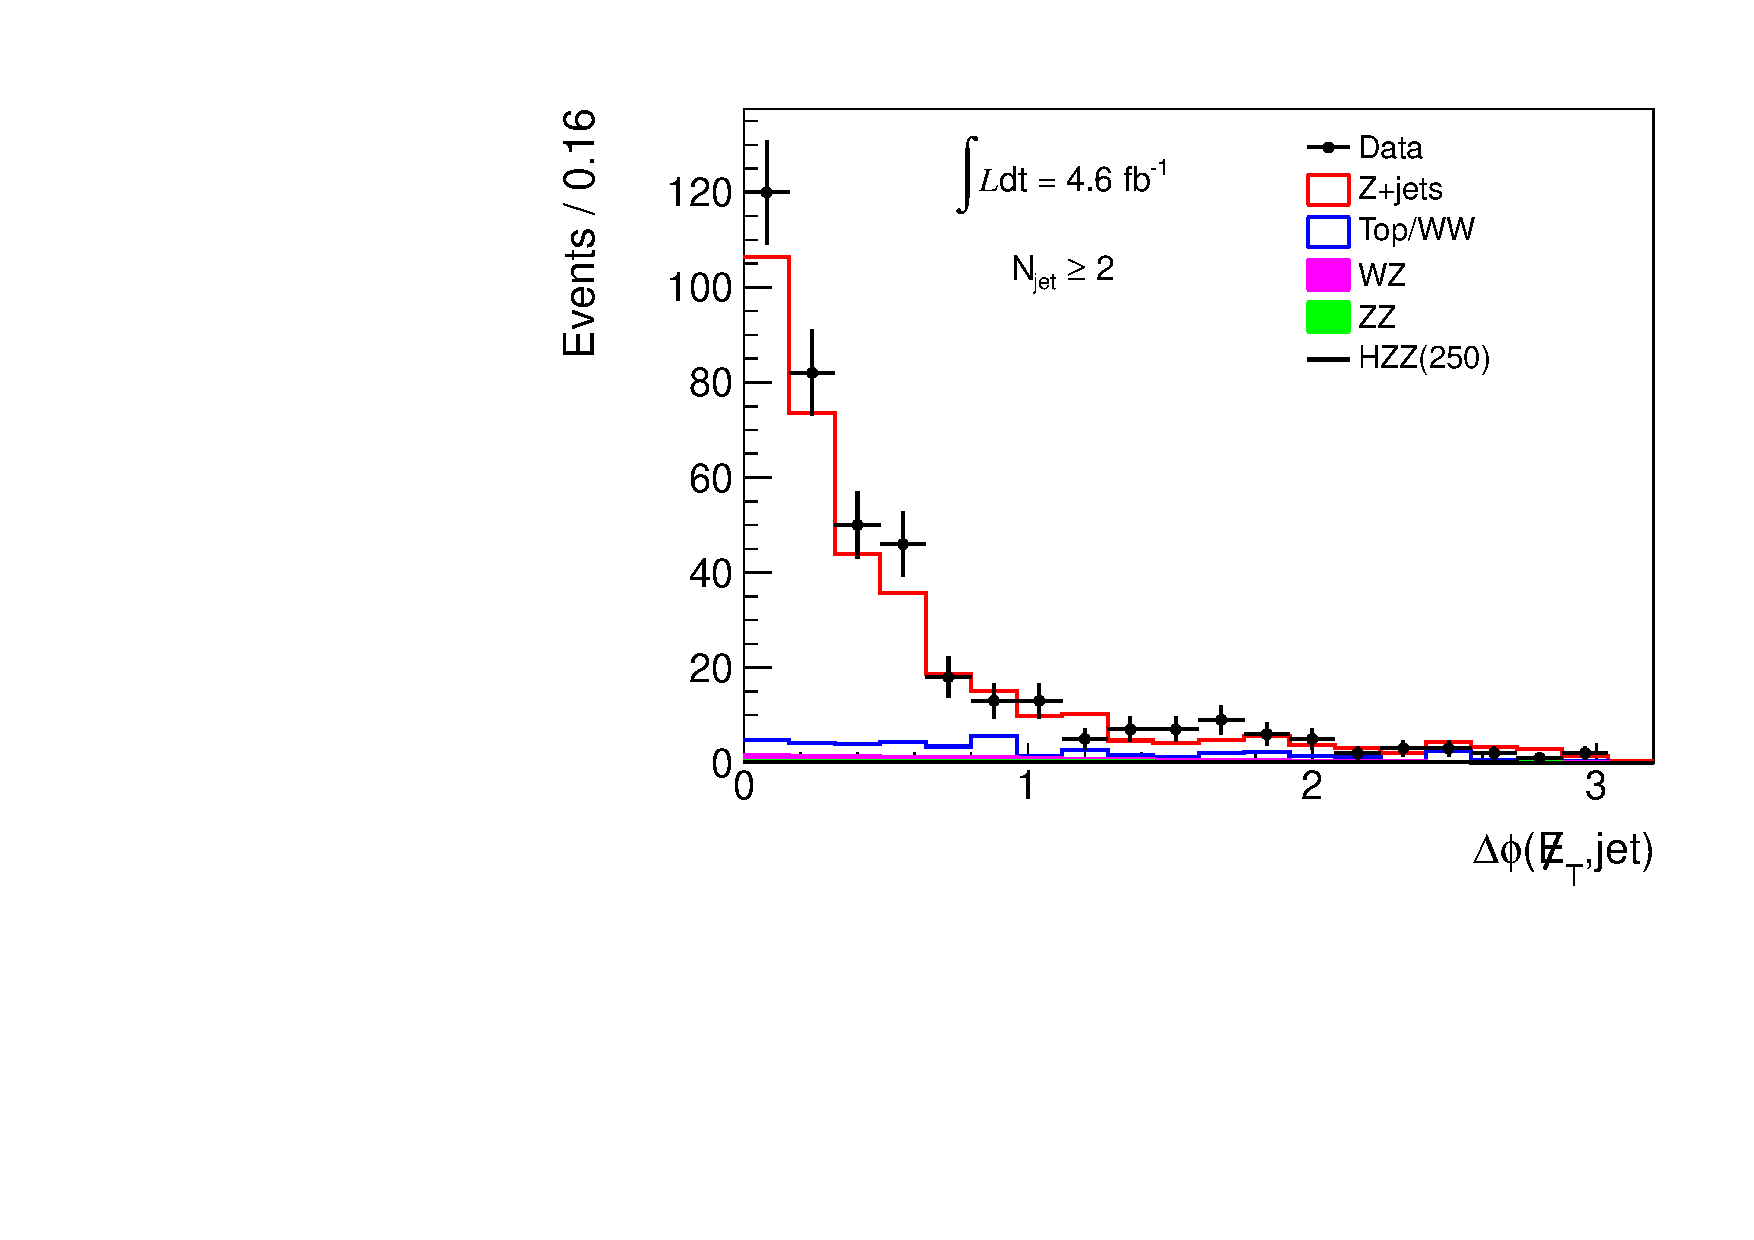
\includegraphics[width=.3\textwidth]{figures/presel_mH250_ee_dphijetmet_2j.pdf}}
\caption{Azimuthal angle separation between \met and the closest jet in the electron channel after the $\ZZ$ preselection observed in data corresponding 
to $4.6$~\ifb data in the $\geq$1 Jets~\subref{subfig:dphijetmet_mm_incl}, 1-Jet~\subref{subfig:dphijetmet_mm_1j} and 
$\geq$2-Jets~\subref{subfig:dphijetmet_mm_2j} bins, compared to the expected from simulation for signal and background. The MC backgrounds are scaled as appropriate and 
the photon+jets estimate of the Z+jets background is added to the stack.}
\label{fig:dphijetmet_zzpresel_ee}
\end{center}
\end{figure}
%%%%%%%%




